%-----------------------------------------------------------------------
%
% File Name: thesis.tex
%
% Author: Thomas Massinger
%
% Revision: $Id$
%
%-----------------------------------------------------------------------

% document class and packages
\documentclass[12pt,notitlepage]{report}
\usepackage{bibunits}
\usepackage{suthesis}
\usepackage{graphicx}
\usepackage{color}
\usepackage{amsmath}
\usepackage{amssymb}
\usepackage{amsfonts}
\usepackage[bookmarksnumbered, bookmarksopen, breaklinks, colorlinks, linkcolor=blue, citecolor=magenta]{hyperref}
\usepackage{subfig}
\usepackage{tabularx}
\usepackage{adjustbox}
%\usepackage{caption}
%\usepackage{rotating}
%\usepackage{tensor}

\pdfoutput=1
\DeclareGraphicsExtensions{.pdf,.png}

\hbadness=10000

% new command definitions
\newcommand{\half}{\frac{1}{2}}
\newcommand{\ospsd}{\ensuremath{S_n\left(\left|f_{k}\right|\right)}}

% journal definitions
\newcommand{\apj}{{\it Astrophysical J.}}
\newcommand{\apjl}{{\it Astrophysical J.}}
\newcommand{\aap}{{\it Astron. and Astrophys.}}
\newcommand{\cmp}{{\it Commun. Math. Phys.}}
\newcommand{\grg}{{\it Gen. Rel. Grav.}}
\newcommand{\cqg}{{\it Class. Quant. Grav.}}
\newcommand{\lr}{{\it Living Reviews in Relativity}}
\newcommand{\mnras}{{\it Mon. Not. Roy. Astr. Soc.}}
\newcommand{\pr}{{\it Phys. Rev.}}
\newcommand{\prl}{{\it Phys. Rev. Lett.}}
\newcommand{\prd}{{\it Phys. Rev. D}}
\newcommand{\pra}{{\it Phys. Rev. A}}
\newcommand{\prsl}{{\it Proc. R. Soc. Lond. A}}
\newcommand{\ptrsl}{{\it Phil. Trans. Roy. Soc. London}}
\newcommand{\rmp}{{\it Rev. Mod. Phys.}}

\newcommand{\tcr}{\textcolor{red}}
\newcommand{\tcb}{\textcolor{blue}}
\newcommand{\tcm}{\textcolor{magenta}}
\newcommand{\tcg}{\textcolor{green}}
\newcommand{\tcp}{\textcolor{purple}}

\begin{document}
\title{Detector Characterization of Advanced LIGO}
\author{Thomas J. Massinger}
\majorprof{Peter R. Saulson}
\previousdegree{}{B.S. Physics, Utica College, Utica, NY 13502}
%\previousdegree{M.S. Syracuse University, Syracuse, NY, 2013}{}
\submitdate{August 2016}
\degree{Doctor of Philosophy}
\program{Physics}
\copyrightyear{2015}
\majordept{Physics}
\havededicationtrue
\dedication{Well that was fun.}
\haveminorfalse
\copyrighttrue
\doctoratetrue
\figurespagetrue
\tablespagetrue
\electronicsubmitfalse

\Abstract{% taken from angular theory paper
Placeholder
}

\Acknowledgments{
I would like to thank many people for all the wonderful things they have done over the past 3000 years or so.

}

\beforepreface

\prefacesection{Preface}
The work presented in this thesis stems from my participation in the LIGO
Scientific Collaboration (LSC). This work does not reflect the
scientific opinion of the LSC and it was not reviewed by the collaboration.



%\vspace*{0.5cm}
%
%\noindent Chapter \ref{ch:photothermal} is based on material from
%
%\vspace*{0.25cm}
%
%\noindent David B. Kelley~{\it et~al.}, ``Observation of photo-thermal feed-back in a stable dual-carrier optical spring,''  to be submitted to
%\prd.
%
%\vspace*{0.25cm}
%
%\noindent Chapter \ref{ch:angular} is based on 
%
%\vspace*{0.25cm}
%
%\noindent David B. Kelley~{\it et~al.}, ``Angular Trap Demonstration,'' to be submitted to
%\prd


\afterpreface

\Chapter{Introduction}
\label{ch:introduction}
% $Id$

In chapter \ref{c:findchirp} we describe in detail the algorithms used to
inspiral signals from binary neutron starts and binary black hole MACHOs in
the LIGO data.  findchirp. We first carefully define the conventions that we
use for analysis quantities in section \ref{s:conventions}; in particular the
definition of the Fourier transform and the power spectral density. Section
\ref{s:waveforms} gives a brief description of the the waveforms used and
section \ref{s:matchedfilter} describes the implementation of the matched
filter.  Spurious noise may cause the output of the matched filter to be large
and so in section \ref{s:chisq} we describe our implementation of the $\chi^2$
time--frequency discriminator proposed in~\cite{allen}. Section
\ref{s:practical} contains additional details of the search particular to our
implementation: the computation of the inverse power spectrum and the trigger
selection algorithm. This is followed by a brief conclusion which summarized
the methods used and outlines some future directions for improvement.

\section{Fourier Transform Conventions}
\label{s:ftconv}

There are two possible sign conventions for the Fourier transform of a time
domain quantity $v(t)$. In this thesis, we define the Fourier transform
$\tilde{v}(f)$ of a $v(t)$ to be
\begin{equation}
\label{eq:ft}
\tilde{v}(f)=\int_{-\infty}^\infty dt\,v(t)\, e^{- 2 \pi i f t}
\end{equation}
and the inverse Fourier transform to be 
\begin{equation}
\label{eq:ift}
v(t)=\int_{-\infty}^\infty df\,\tilde{v}(f)\, e^{2 \pi i f t}.
\end{equation}
This convention differs from that used in some gravitational wave literature,
but is the adopted convention in the LIGO Scientific Collaboration.


\Chapter{Searching for Compact Binary Coalescences}
\label{ch:CBCSearches}
Since a signficant portion of this thesis uses the performance of 
CBC searches as a metric for the quality of the 
data, a more thorough discussion of how a CBC search 
works is necessary. This thesis will focus on the output of the PyCBC 
pipeline, which is a Python-based software packaged used to search for 
gravitational waves from compact binary coalescences \cite{Usman:2015kfa,pycbc-github}.

CBC search pipelines are designed to search for gravitational wave transients 
from compact binary coalescences \cite{Usman:2015kfa}. 
The signals expected to be measured in the LIGO interferometers are extremely quiet, 
with gravitational wave strains on the order of $10^{-22}$. On these scales, most 
signals will not be able to be extracted from the background noise with simple filtering. 
Figure \ref{fig:quiet-BNS} shows the gravitational wave strain from a 1.4-1.4$M_{\odot}$ 
binary neutron star system at a distance of 20 Mpc overlaid on real detector noise from 
the Livingston 
interferometer. The signal has a peak strain roughly two orders of magnitude lower than 
the peak strain of the detector noise. 
For this reason, the CBC searches employ a matched filter algorithm, which correlates 
expected CBC
waveforms with detector data and assigns a ranking statistic, the signal-to-noise 
ratio (SNR), to every event that it finds. 

\subsection{The matched filter}

The matched filter calculates the correlation of the detector data with expected CBC 
waveforms in the frequency domain. The detector data and expected waveform are 
multiplied together and their product is divided by the background noise in the detector. 
The fundamental operation of the matched filter is defined as an inner product of the 
detector data and the CBC waveform \cite{Allen:2005fk},
\begin{equation}
(s|h)(t) = 4\mathrm{Re}\int_{f_\mathrm{low}}^{f_\mathrm{high}} \frac{\tilde{s}(f)\tilde{h}^*(f)}{S_n (f)}e^{2\pi i f t}\, \mathrm{d}f,
\label{eq:inner-product}
\end{equation}
where $\tilde{s}$ is the Fourier transformed detector data, $\tilde{h}$ is the Fourier
transformed gravitational waveform, and $S_n (f)$ is the power spectral
density of the detector data averaged over 2048 seconds, which represents the average 
noise in the detector. The maximum bounds of the integral are set to span the frequency space 
for which the interferometers are sensitive enough to detect gravitational waves, 
typically 30 - 2000 Hz. However, if a waveform merges at a lower frequency, the upper bound 
on the integral can be set to capture the frequencies where the signal has power and 
nothing higher.

As described in Equation \ref{eq:strain}, a gravitational wave is comprised of two 
polarizations, ``h-plus" and ``h-cross". When the data are searched for a CBC  
signal, a waveform is generated for each polarization and the matched filter is 
computed separately for each polarization. 
The SNR of a CBC waveform at any given time is defined as the weighted quadrature sum 
of the SNR measured for each polarization \cite{Allen:2005fk}, 
\begin{equation}
\rho^2(t) = \frac{(s|h_\mathrm{p})^2 + (s|h_\mathrm{c})^2}{(h_\mathrm{p}|h_\mathrm{p})},
\label{eq:snr}
\end{equation}
where $h_\mathrm{p}$ and $h_\mathrm{c}$ are the plus and cross polarizations of the 
modeled gravitational waveform respectively and $s$ is the detector data. 
When the SNR time-series defined in equation \ref{eq:snr} crosses a certain threshold, 
the waveform is considered to have significant overlap with the detector data and an 
event is generated at the time of the SNR peak. These events are called ``triggers'' 
and are used to generate populations of potential gravitational wave events for analysis.

\begin{figure}[ht!]
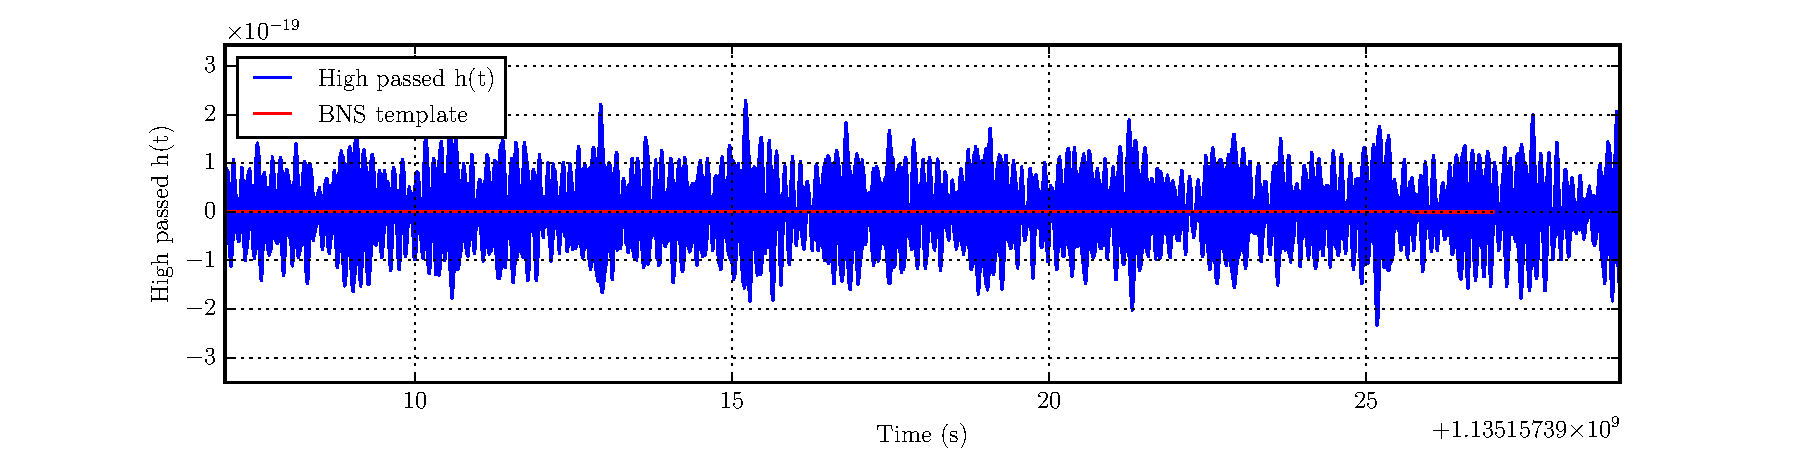
\includegraphics[width=\textwidth]{figures/introduction/quiet_BNS}
\caption[BNS signal in detector noise]{A simulated gravitational wave signal from a %
         binary neutron star system overlaid on real detector noise from L1. %
         The blue curve, labeled $h(t)$, represents the detector data. %
         The red curve represents %
         the gravitational wave strain expected from a 1.4-1.4$M_{\odot}$ %
         binary neutron star system %
         at 20 Mpc. The peak strain of the binary neturon star waveform is %
         $8\times10^{-22}$. %
         The detector data have been high pass filtered with a corner frequency %
         at 20 Hz and show a peak strain of $2.2\times10^{-19}$. The signal is %
         buried in the detector noise and requires a matched filter algorithm %
         to be recovered. At this time, the inspiral range for a 1.4-1.4$M_{\odot}$ %
         BNS system was 60 Mpc, indicating that the same system originating at 60 Mpc %
         would be recovered with SNR = 8. % 
         }
\label{fig:quiet-BNS}
\end{figure}

\subsection{Waveform templates}

To perform a search, the matched filter algorithm needs to know what to search for.
A collection of expected CBC waveforms is generated using
the formalism of general relativity before the analysis \cite{Pan:2009wj,Purrer:2015tud}.
Each of the expected waveforms is called a template and
the full collection of waveforms is referred to as the template bank. This template bank
is constructed to span the astrophysical parameter space included in the search
\cite{GW150914-CBC}. This parameter space is constrained by the noise spectrum of 
the interferometers. As shown in Figure \ref{fig:noise-budget}, the LIGO 
interferometers are sensitive enough to detect gravitational waves in the 
region from roughly 30 - 2000 Hz. This rules out detection of sources that are expected to 
coalesce at very low frequencies, such as supermassive black hole binaries 
\cite{Merloni:2008tj} and 
binary white dwarf systems \cite{PostnovYungelson:2006}. 
The template bank used in Advanced LIGO's first observing 
run consisted waveforms representing binary neutron stars, binary black holes, 
and neutron star-black hole binary systems \cite{GW150914-CBC}. 
The total masses of these systems ranged from 
2-100$M_{\odot}$. This reflects the set of systems that will have merger frequencies 
above 30 Hz and will have detectable power in LIGO's sensitive bandwidth.

Each waveform is defined by the mass and spin of each compact
object in the binary system. 
It is convenient to combine
the component masses into a new variable, chirp mass, which is used to
parameterize gravitational wave signals in general relativity. Chirp mass is defined
as \cite{PhysRev.131.435}
\begin{equation}
M_{chirp} = \frac{(m_1m_2)^{3/5}}{(m_1 + m_2)^{1/5}}
\end{equation}
where the $m_{i}$ are the component masses of the compact objects in the
binary system. 
Each compact object in the binary system has its rotation represented by a 
dimensionless spin parameter,
\begin{equation}
\chi_i = \frac{cS_i}{Gm_i^2},
\end{equation}
where $S_i$ is the spin angular momentum of the compact object, $m_i$ is the mass 
of the compact object, c is the speed of light, and G is the gravitational constant. 
It is convenient to combine the effects of each
object's spin into one parameter called effective spin, $\chi_{eff}$,
which is the
mass-weighted spin of the system \cite{Privitera:2013xza}. $\chi_{eff}$ is defined as
\begin{equation}
\chi_{eff} = \frac{\chi_{1}m_{1} + \chi_{2}m_{2}}{m_{1} + m_{2}}
\end{equation}
where the $\chi_{i}$ are the dimensionless spin parameters \cite{Kidder:1995zr}
and the $m_{i}$ are the masses for each compact object in the binary system. 


\subsection{$\chi^{2}$ signal consistency test}\label{sec:chisq}

If the data produced by the interferometers were Gaussian, the matched filter would 
be sufficient for running a search pipeline and recovering gravitational wave signals. 
Unfortunately, the data are non-Gaussian, containing noise transients of varying 
durations \cite{Nuttall:2015dqa,GW150914-DETCHAR}. These noise transients, 
or ``glitches", can have significant amplitude 
and, when multiplied with a waveform template in the matched filter, can cause 
loud triggers to be generated. 
However, a significant advantage of performing a modeled search for gravitational 
waves is that 
we know we're looking for. With this information, the SNR can be refined into a more 
robust ranking statistic for significant events in the data. This is done using the 
$\chi^{2}$ signal consistency test \cite{Allen:2004gu}. 

The SNR produced by the matched filter is an integral in the frequency domain which 
reports the total accumulated SNR over a given bandwidth. If a noise transient has 
significant amplitude, it can generate a high SNR trigger by overlapping with the 
waveform template in the matched filter. However, these noise 
transients typically have a duration on the order of 0.1s. This type of transient 
is easily distinguished from a chirp signal that increases monotonically in frequency 
over the span of many seconds. Figure \ref{fig:bbh-with-blip} shows an example of such 
a noise transient with the waveform of a binary black hole system overlaid on top of it. 
Although the peaks of each time-series are aligned, the noise transient clearly has a more 
localized power distribution that does not match that of the CBC waveform.

\begin{figure}[ht!]
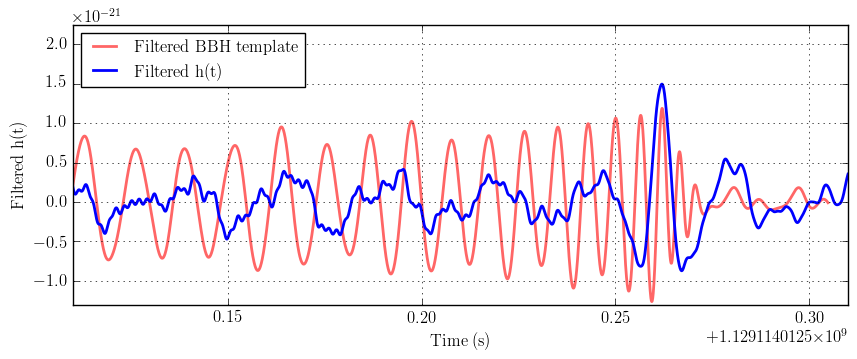
\includegraphics[width=\textwidth]{figures/introduction/bbh-with-blip}
\caption[Transient with BBH waveform]{A time domain representation of a noise transient in the %
         L1 detector with a binary black hole waveform overlaid on top of it. Both %
         time-series have been filtered to isolate the frequencies where the glitch % 
         and the waveform have significant power. The peak amplitude of the binary %
         black hole waveform lines up with the peak amplitude of the noise transient %
         in the detector data, $h(t)$. However, the binary black hole waveform contains %
         many more cycles than the noise transient. It is clear that this transient does %
         not have the same distribution of power in time and frequency as the CBC signal.}
\label{fig:bbh-with-blip}
\end{figure}

The $\chi^{2}$ test divides each CBC waveform into
frequency bins of equal power, checking that the SNR is distributed as a 
function of frequency
as expected from an actual CBC signal.
For a signal divided into $p$ frequency bins, each bin should contain $\frac{1}{p}$ of the power in the 
signal. 
In the $\chi^2$ calculation, the SNR is calculated for each frequency bin and compared to the expected 
amount. The $\chi^2$ statistic is calculated as \cite{Usman:2015kfa}
\begin{equation}
\chi^2 = p\displaystyle\sum_{l=1}^{p}\left[\left(\frac{\rho_\mathrm{p}^2}{p}-\rho_{\mathrm{p},l}^2\right)^2 + \left(\frac{\rho^2_\mathrm{c}}{p}-\rho_{\mathrm{c},l}^2\right)^2 \right] \, ,
\label{eq:chisqr}
\end{equation}
where $\rho^2_\mathrm{p}$ is the SNR of the plus polarization of the waveform, $\rho^2_\mathrm{c}$ 
is the SNR of the cross 
polarization of the waveform, $p$ is the number of frequency bins, and 
$\rho^2_{i,l}$ is the calculated SNR for the $l^\mathrm{th}$ frequency bin.
The $\chi^2$ statistic is then normalized such that a real signal will be reported with a value of 1. 
This normalized $\chi^2$ is called the reduced $\chi^2$ and is denoted by $\chi^2_r$.

In the PyCBC search, each trigger that comes out of the matched filter search is 
weighted based on the results of
the $\chi^{2}$ test. This is folded into a new ranking statistic for CBC triggers,
which is called re-weighted SNR and is denoted by $\hat{\rho}$.
The re-weighted SNR is calculated as \cite{Usman:2015kfa} 
\begin{equation}
\hat{\rho} = \left\{\begin{array}{lr}
\rho\left/\left[(1+(\chi^2_r)^3)/2\right]^\frac{1}{6}\right., & \text{if } \chi_r^2 > 1, \\
\rho, & \text{if } \chi_r^2 \le 1,
\label{eq:reweighted}
\end{array}\right.
\end{equation}
where $\rho$ is the measured SNR and $\chi^2_r$ is the reduced $\chi^2$.
It is important to note that if a real signal has a power
distribution that matches the template waveform, it will not be
down-weighted by the $\chi^{2}$ test.  

This test is extremely powerful, as shown in Figure \ref{fig:cbc-newsnr-histograms}, 
which shows the distribution of single detector PyCBC triggers generated from 
September 12 to October 20, 2015. 
Figure \ref{subfig:l1-snr-hist} shows the distribution of triggers in SNR. 
The extensive tail of
triggers with high SNR, which is generated when high amplitude noise transients 
are processed by the matched filter, extends beyond SNR 100. 
These high SNR triggers are down-weighted in the re-weighted SNR distribution,
leaving behind a tail that extends to $\hat{\rho} \approx$ 11.5 as seen in Figure 
\ref{subfig:l1-newsnr-hist}. Keeping in mind that a real signal will be reported 
at the same value in each plot, the re-weighting of triggers has lowered the 
noise floor, allowing for signals with SNR $>$ 11.5 to stand out as the 
loudest events in their respective interferometers rather than being buried 
beneath a population of high SNR triggers.  

\begin{figure}[!ht]%
\centering
  \subfloat[]{
      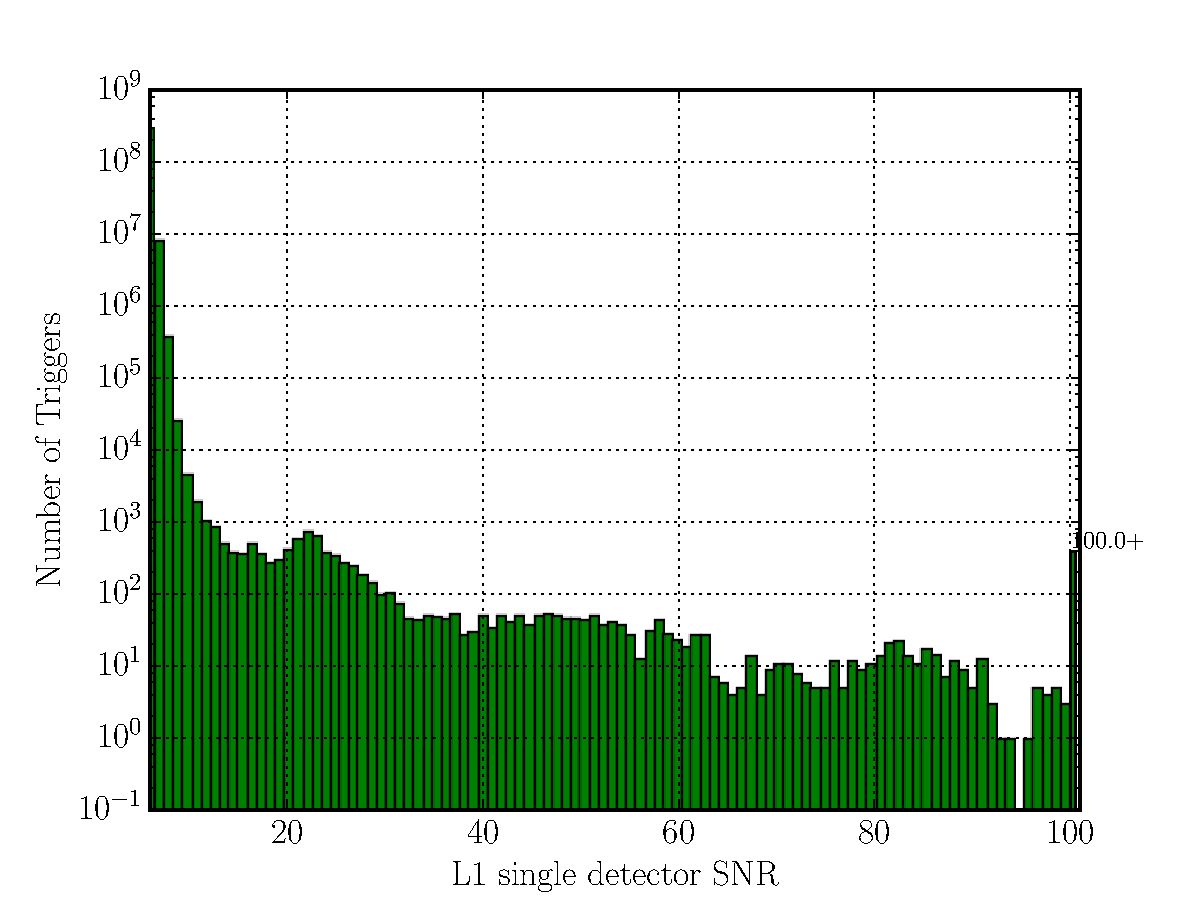
\includegraphics[width=.75\textwidth]{figures/introduction/l1-snr-histogram}
      \label{subfig:l1-snr-hist}
  }

  \subfloat[]{
      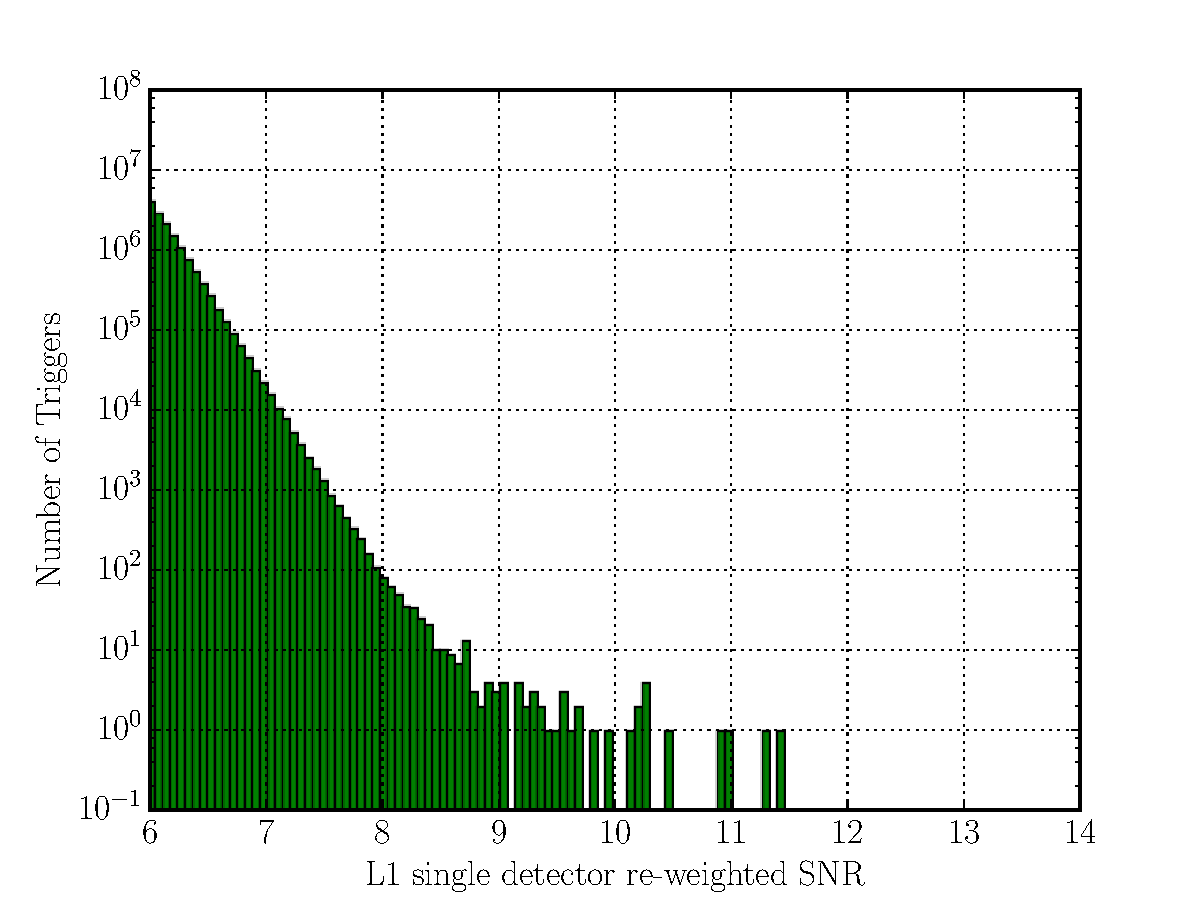
\includegraphics[width=.75\textwidth]{figures/introduction/l1-newsnr-histogram}
      \label{subfig:l1-newsnr-hist}
  }

  \caption[PyCBC SNR and re-weighted SNR histograms]{Histograms of single interferometer PyCBC %
           triggers from the Livingston (L1) interferometer. %
           These triggers were generated from September 12 to October 20, 2015. These histograms %
           contain triggers from the entire template bank, but %
           exclude any triggers found in coincidence between the two interferometers. %
           (\ref{subfig:l1-snr-hist}) A histogram of single interferometer triggers in SNR. %
           The tail of this distribution extends beyond SNR = 100. %
           (\ref{subfig:l1-newsnr-hist}) A histogram of single interferometer triggers in re-weighted SNR. %
           The chi-squared test down-weights the long tail of SNR triggers %
           in the re-weighted SNR distribution. Note that the x-axis has different %
           limits in each plot.}
  \label{fig:cbc-newsnr-histograms}
\end{figure}

The remaining tail of re-weighted SNR triggers represents the loudest 
background triggers in the CBC search. Investigating this set of
loudest background triggers guides data quality efforts in defining the current 
limiting noise sources to the CBC search. This process is detailed in Chapter 
\ref{ch:instrumentalDetchar}.

\subsection{Searching for signals}

The matched filter algorithm is run separately on each interferometer's data using the 
same bank 
of template waveforms. The output of the matched filter, the SNR time-series, is scanned 
for peaks and a set of single interferometer 
triggers is generated. The two sets of single interferometer triggers are then compared to
search for any events that were recorded within 15ms of each other with the same mass and 
spin parameters. 
Gravitational waves are predicted by general relativity to travel
at the speed of light. The light travel time between the two interferometers is 10 ms
and 5ms is added to the coincidence window due to uncertainty in signal arrival time
\cite{GW150914-CBC}.
As such, any triggers that are found within 15 ms of each other and
are recovered with the same source parameters are considered to be coincident between 
the two
interferometers. These coincident triggers represent potential gravitational wave signals
and are referred to as candidate events. 

The ranking statistic for coincident events in the PyCBC search is the network
re-weighted SNR, $\hat{\rho}_{c}$, which is the quadrature sum of the re-weighted
SNR from each interferometer.  
\begin{equation}
\hat{\rho}_{c} = \sqrt{\hat{\rho}^2_L + \hat{\rho}^2_H}
\end{equation}
where $\hat{\rho}_L$ is the re-weighted SNR measured in the Livingston detector 
and $\hat{\rho}_H$ is the re-weighted SNR measured in the Hanford detector.

Most of these foreground events will be
chance coincidences between noise in each interferometer, which is expected given
the number of events in each data set. A large number of foreground events will be 
generated due to the detector noise, but ideally the distribution of foreground events 
will fall of sharply in $\hat{\rho}_{c}$ as shown in Figure \ref{fig:pycbc-hist-gw150914}, 
allowing for genuine signals to be 
recognized. To understand how stastically significant a foreground event is, a background 
distribution must be generated to calculate how often such a signal will be produced based 
on instrumental noise.

To generate the background distribution, we return to the set of single interferometer 
triggers that were generated when the matched filter was initially run. Since we want 
to understand the distribution of triggers based on detector noise, all of the triggers 
that were found to be coincident between the two interferometers are removed from the 
data sets, effectively removing all
potential gravitational wave signals. The remaining triggers are then due to fluctuations 
in the background noise in each interferometer. These two sets of triggers,
one from each interferometer, are then time shifted by a duration longer than the
light travel time between the interferometers.
Since gravitational waves are predicted to travel at the speed of light,
this time shift ensures that the
two sets of triggers are astrophysically uncorrelated and do not contain any gravitational
wave signals. The coincidence test is then performed again with the time shifted triggers,
resulting in a coincident trigger set which represents background noise. 
A full distribution of background triggers is generated by performing this timeslide
technique every 0.1 seconds and iterating over all of the data used in the search 
\cite{Usman:2015kfa}. This 
distribution tells us how often we should expect to see coincident triggers with the 
same waveform parameters at a given value of SNR.

The statistical significance of any candidate gravitational wave is
evaluated by calculating the rate of background events from detector noise 
that are at least as
loud as the candidate event \cite{GW150914-CBC}. 
The results of the first observing run and details on 
the significance of foreground events is presented in Chapter \ref{ch:o1results}. 
Any loud triggers that appear as the result of instrumental
transients will contribute to the tail of the background distribution and
the influence the statistical significance of a recovered foreground event.
The process of performing data quality investigations and data validation are 
detailed in Chapter \ref{ch:instrumentalDetchar}

\subsection{Gating}\label{sec:gating}

The PyCBC search includes a data conditioning stage that applies preventative  
cuts to remove large transients from the input data stream. 
This is done in a process called gating \cite{Usman:2015kfa}, which uses a
window function to remove times containing large transients from the input data stream. 
This windowing function smoothly rolls the problematic section of data to zero, excising the large transient.
The gating process is tuned by modifying the selection criteria for transients to be removed and
by adjusting the time window to remove around each transient.
Chapters \ref{ch:GW150914-DQ} and \ref{ch:GW151226-DQ} contain details about the 
gating thresholds used for the analyses containing GW150914 and GW151226 respectively. 



\Chapter{The First Observing Run}
\label{ch:o1results}
\section{O1 results}

We found GW150914!




\Chapter{Detector Characterization}
\label{ch:instrumentalDetchar}
\section{Methods of Detector Characterization}

The Detector Characterization (DetChar) group works at the interface 
between the instrument science and data analysis groups. The goal of 
the group is to understand the effects of instrumental noise sources on 
the output of astrophysical searches and mitigate them if possible.

The first step in a detector characterization study is identifying 
noisy or problematic data. These studies can be initiated in a number of ways. 
The three most common are the appearance of 
loud background events in an astrophysical search pipeline, a message from 
the commissioning team regarding instrument performance, or excess noise 
flagged by data quality monitoring software. Section \ref{sec:tools} discusses 
the data quality monitoring software further.

There are a large number of recorded signals used to monitor and control the
interferometers that are not used in astrophysical searches. These auxiliary
channels are considered safe to use for noise characterization because they are
not sensitive to gravitational wave signals. Analyses of auxiliary channels
allow for the identification of systematic noise sources \cite{Smith:2011,Isogai:2010},
such as environmental
disturbances \cite{Effler:2014zpa} or excess motion of auxiliary optics in the
interferometer \cite{GW150914-DETECTORS,InstrumentNoisePaper}. 

Once data with excess noise have been identified, they must be characterized 
in order to track down the source of the noise. A number of questions can 
be asked to characterize the noise. Is the noise transient or a slow 
drift? What is the typical frequency and bandwidth of the noise? Does the 
noise follow a power law in frequency? Does the 
noise have a characteristic shape in the time-frequency plane? Are the 
noisy frequecies of the signal coherent with other signals in the instrument 
such as environmental monitors and optical control signals? 
Is the noise source localized to a specific chamber or does it exist at 
multiple physical locations in the interferometer? Does the characteristic 
frequency match any of the known mechanical resonances in the interferometer? 
If the noise is a slow drift, does it correlate with the slow drift of 
other signals in the interferometer? Does the noise seem highly digital 
or discretized? After gathering all available information about the 
character of the noise and its coupling mechanisms, efforts shift 
toward attempting to mitigate the effects of the noise on search 
pipelines. 

There are two primary ways to mitigate the effects of instrumental noise on 
the output of a search pipeline. The first option, which is highly preferred, 
is to track down the source of the noise in the interferometer and fix the 
problem at its origin. If investigations provided enough information that 
a problem can be traced back to a specific piece of electronics or a 
specific control loop, the problem can be fixed at the source. However, 
this is not always possible since instrument noise can be difficult to 
pin down and hardware repairs are often too invasive to perform during 
an observing run.

If the problem cannot be fixed at the source, the second option is to 
remove the problematic data from the astrophysical analyses. 
When a significant noise source has
been identified using auxiliary channels and cannot be repaired immediately, 
a data quality flag can be generated
to indicate times when the output data from the interferometer is not nominal
\cite{Nuttall:2015dqa,S6DetChar,GW150914-DETCHAR,Amaldi}.
Data quality vetoes are discussed further in section (??).  
If possible, it is always preferable to fix a problem at the source. 

\section{Tools and algorithms}\label{sec:tools}

Identifying and characterizing instrument noise is facilitated by a 
suite of software tools and algorithms designed to flag data with 
excess noise and help correlate this noise with other signals in the 
interferometer. The major tools required for understanding the data 
quality investigations in this thesis are discussed below. 

\subsection{Omicron}

One way to quantify the amount of excess noise in $h(t)$ is to look 
for times where the signal contains excess power using 
Omicron, a burst algorithm. 

Omicron applies a whitening filter to $h(t)$ and projects it into 
a sine-Gaussian basis. Each sine-Gaussian basis function is defined 
by a central time, $t_0$, a central frequency, $f_0$, and a Q-factor, 
which is defined as 
\begin{equation}
Q = \frac{f_0}{\Delta f} = 4\pi f_0 \Delta t,
\end{equation} 
where $\Delta t$ is the time duration of the sine-Gaussian and 
$\Delta f$ is the bandwidth of the sine-Gaussian. Using these parameters, 
each sine-Gaussian basis function can be represented as a tile in the 
time-frequency plane centered around $t_0$ and $f_0$, where the width of 
the tile is determined by the time duration 
and height of the tile is determined by the frequency bandwidth. 

For each 
of these tiles, the energy is measured and compared to the median tile 
energy. If there is an excess of energy in a given tile relative to the 
median tile energy, a signal-to-noise ratio (SNR) is calculated and a trigger 
is generated to annotate the event. For each trigger, the SNR, central time, 
central frequency, duration, bandwidth, and Q of the tile are recorded. 

Once the data have been decomposed into the full set of basis functions, the 
resulting set of triggers is sent through a clustering algorithm. This is 
necessary because the set of sine-Gaussians is an overcomplete, 
non-orthogonal basis and a single event in the data can generate multiple 
triggers corresponding to different values of $t_0$, $f_0$, and Q. The 
resulting clustered triggers define the peak time, peak frequency, and 
SNR of a cluster as the central time, central frequency, and SNR of the 
most significant tile in the cluster. 

The most useful way to visualize the output of Omicron is in the 
time-frequency-SNR plane, sometimes referred to as a 'glitchgram', 
where each trigger is represented as a point 
in a scatterplot. Figure \ref{fig:glitchgram} shows an example set of 
Omicron triggers in the time-frequency-SNR plane. Each dot represents 
a trigger at a certain peak time and peak frequency. The color of each 
dot represents the SNR of that trigger. 

In Gaussian noise, the SNR of a 
given trigger is not expected to exceed 8. In this example, there are a number 
of triggers with SNR $> 8$, some with noticeable structure and some that seem 
more randomly scattered, that represent noise in the output of the interferometer. 
For example, there are numerous triggers between 10-20 Hz that represent excess noise at 
these frequencies, likely due to scattered light in the 
interferometer. There is a line of triggers at just above 2kHz that indicates 
a noise source with a constant peak frequency whose amplitude is being modulated 
and a high SNR is being reported. There is also a scattering of points with high 
SNR that are not as structured as the previous two examples, each one likely due 
to an individual loud glitch rather than a constant, systematic noise source.

\begin{figure}[ht!]
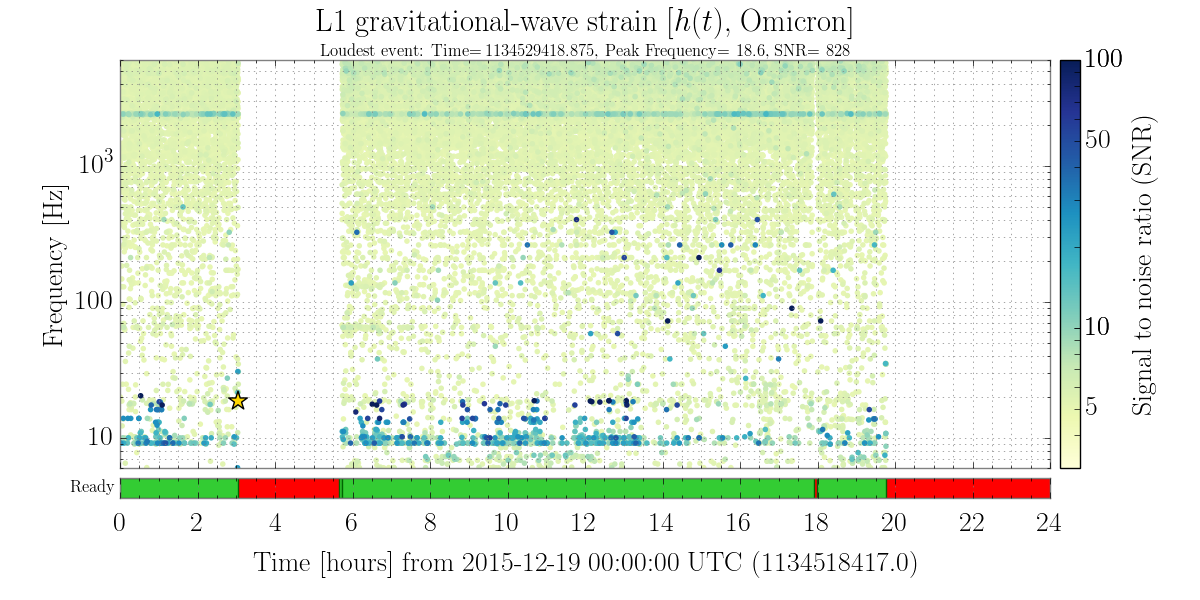
\includegraphics[width=\textwidth]{figures/detchar/Omicron-Dec19}
\caption[Omicron time-frequency-SNR plot]{Time-frequency-SNR plot of Omicron triggers.}
\label{fig:glitchgram}
\end{figure}

The results of Omicron are a commonly used and extremely valuable tool 
for characterizing the noise in the instrument. A cursory glance at 
Figure \ref{fig:glitchgram} identifies 3 populations of noise in 
the instrument, each of which can be followed up on individually 
to discover both the source of the noise and its effect on astrophysical 
searches. Omicron triggers can also be used in statistical analyses to 
find correlated noise between auxilary channels and $h(t)$. An often used 
example of this, Hierarchichal Veto, is discussed below. 

\subsection{Hierarchichal Veto}

One tool that we have often used in Detector Characterization to look 
for time coincidence between noise transients, or 'glitches', in auxilary 
channels and the output of the interferometer is Hierarchical Veto (Hveto). 
Typically, Hveto is used to compare a channel that potentially contains 
gravitational wave signals, denoted $h(t)$, and an auxiliary channel 
that does not have direct astrophysical implications. Hveto counts 
the number of coincident triggers between two time series using a 
user-defined time window centered around each trigger in the auxiliary 
channel. The figure of merit returned by Hveto for each auxiliary channel 
after comparison to $h(t)$ is called \textit{significance}.

Significance answers the following question: how unlikely is it that 
the coincident triggers in these two channels were the result of 
two arbitrary Poisson processes occurring in each channel? 
More specifically, given two arbitrary Poisson processes, how 
unlikely is it that we measure $n$ or more coincident triggers 
given that expected number of coincidences from random chance is $\mu$?

Significance is calculated as (ref Hveto),
\begin{equation}
S = -\log_{10} (\sum\limits_{k = n}^{\infty} P(\mu,k)),
\end{equation}
where $n$ is the number of coincidences found between the two channels 
during the total analysis time and $P(\mu,k)$ is the Poisson probability 
distribution function,
\begin{equation}
P(\mu,k) = \frac{\mu^{k}e^{-\mu}}{k!},
\end{equation}
where $\mu$ is the expected number of coincidences between triggers in 
$h(t)$ and the auxiliary channel based solely on chance, which is estimated as,
\begin{equation}
\mu = \frac{N_{h}N_{aux}T_{win}}{T_{tot}},
\end{equation}
where $N_{h}$ and $N_{aux}$ are the number of triggers in $h(t)$ and a 
given auxiliary channel respectively, 
$T_{tot}$ is the total analysis time, and $T_{win}$ is the length of the 
coincidence window used.

A high value of significance indicates that the triggers in the channels 
were very often coincident in time and that there is a very small probability 
that their intersection is a product of random chance. This is a very useful 
measure when we are searching for auxiliary channels that might have some 
noise coupling into our output channel. A significance value of up to 5 is 
often observed in channels with no causal relationship to $h(t)$ (ref Hveto), 
which is a useful threshold for identifying effective vetoes.

Another interesting figure of merit used for a given comparison Hveto is 
the ratio of $\frac{efficiency}{deadtime}$. Efficiency is defined as the 
percent of triggers vetoed from $h(t)$ during a round of vetoes. Deadtime 
is defined as the percent of total analysis time removed from $h(t)$ during 
a round of vetoes. A ratio of 1 is what we would expect from vetoing time 
at random, indicating no strong time correlation between triggers in the 
two channels. A high value of this ratio, which is ideal, indicates that 
we are vetoing a large number of triggers while maintaining a high percentage 
of our analysis time. This means that the triggers are often close enough 
in time that we can catch a large number of triggers using a small time window.

The deeper utility of Hveto is made evident when a channel is found to have 
a strong correlation with $h(t)$. 
When Hveto discovers an auxiliary channel that has a strong correlation 
with $h(t)$, which is called the round winner, it removes all of the time 
windows surrounding 
auxiliary channel glitches and recalculates the significance of the list of 
auxiliary channels. If a channel's significance has dropped after this removal 
of time, it must have had a large amount of glitches coincident with the 
round winner. The change in significance of each channel is displayed on a 
figure called a `drop-plot`. This is one of the most powerful features of Hveto
 - the ability to find families of channels that often glitch at the same time. 

Ideally, the list of significant channels displayed on the drop-plot will be 
able to localize the issue to a specific subsystem or area of the IFO. 
For example, if a channel representing the alignment of the input mode 
cleaner has glitches that are strongly correlated to $h(t)$, it would be 
interesting to look at the drop-plot and find out what other channels are 
glitching at the same time (suspensions, laser power, etc.).
From there, the issue can be investigated and brought to the attention of 
commissioners for repair or physical inspection. This is not always possible 
as sometimes the cause of the glitches is unclear, but identifying times of 
poor data quality is still useful.

Using Hveto, we can monitor auxiliary channels to find and remove glitches 
in $h(t)$ that would otherwise pollute a gravitational-wave analysis. Removing 
these glitches serves multiple purposes for the search pipelines. Removing 
high SNR glitches cleans up search backgrounds and allows the search 
pipelines to claim a lower SNR threshold for potential detections. A lower 
SNR threshold implies a larger volume for astrophysical analysis. Removing 
glitches reduces the potential for false alarms in the search pipelines, 
which in turn increases the confidence of eventual detections.

\section{Instrumental Detector Characterization Studies}

\subsection{Analog-to-Digital Conversion}

Advanced LIGO interferometers are controlled in real-time using a digital 
control system installed on a series of computers referred to as front end 
computers.  This system overall is referred to as the Front End Control 
(FEC) subsection of the more expansive Control and Data System (CDS).  
In a control loop, the FE computers must be capable of reading in an 
analog signal from the interferometer (position measurements, error signals, 
coil currents, etc), digitally sampling that analog signal, using these now 
digital values in a series of control algorithms, and outputting an analog 
control signal to send back into the interferometer.

The process of digital sampling is handled by an analog-to-digital 
converter (ADC) and the process of analog output is handled by a 
digital-to-analog converter (DAC).  Since these converters are linearly 
mapping a continuous signal onto a discrete range, they are limited by 
their digital bit depth.  For example, a 16 bit ADC is only capable of 
representing $2^{16}$ discrete values, or a range from zero to 65536.  
This range is often centered around zero, giving the ADC the capability 
to handle a range of $\pm32768$.  An incoming analog signal is mapped 
onto this range and converted into a digital signal.

For example, in sampling an analog signal with a range of $\pm20V$, 
10V would be mapped to 32768 digital counts and -10V would be mapped 
to -32768 digital counts with all 
of the intermediate voltage values being linearly mapped to the range. This 
means our digital system would recognize a discrete step size of 
10V/32768 counts $\approx 305 \mu $V/count.

Looking at the system described above, we must be aware of how our system 
is going to react when our analog input signal exceeds the intended maximum 
value of 10V (e.g., an 11V input). The ADC has already assigned its maximum 
digital value to 10V. This is called a digital overflow. In this case the ADC 
will continuously output its maximum value as it has no way to map 11V into 
a discrete value. The same process can occur in a DAC when a digital signal 
is sent out at the maximum allowed digital value. The resulting analog signal 
will be railed at the maximum output value of the DAC, creating a sharp corner 
in the output signal as it flattens out. 

If the digital system is not able to correctly sample and understand an analog 
error signal, it is easy to imagine a scenario where the reponse of the digital 
system and the output control signal are not able to complete the control loop 
as designed. This may cause glitches or misalignments in the interferometer.
We must also consider the fact that many ADCs are calibrated to reflect the 
intended dynamic range of an optic.  If a saturation is occurring, there is 
a good chance that an optic has moved beyond this intended dynamic range, which 
also may cause glitches or misalignments.

The ADCs and DACs are monitored by a series of auxiliary channels, which are 
automatically generated in the front-end system. These auxiliary channels 
monitor each ADC and DAC channel and note when any of the channels has reached 
its digital limit. These channels can be used to generate flags that mark 
ADC and DAC overflows, which can be compared with glitches in $h(t)$ to 
search for glitch mechanisms driven by overflows. These channels can also 
be used to flag any large glitches that cause digital overflows so that they 
can be removed from astrophysical searches. 

Figure \ref{fig:dac-overflow} shows an example of a large glitch that caused 
a digital overflow and was removed from gravitational wave analyses. Figures 
\ref{subfig:strain-dac-overflow} and \ref{subfig:esd-dac-overflow} show a 
large glitch in $h(t)$ and the response of a drive signal that controls 
the motion of ETMY respectively. The signal in \ref{subfig:esd-dac-overflow}, 
which is supposed to be controlling the motion of ETMY, hits its digital 
limit during this glitch. Figure \ref{subfig:etmy-dac-overflow} shows the 
auxiliary channel that monitors this digital overflow incrementing as 
it witnesses the digital overflow. 

\begin{figure}[ht!]%
\centering
\subfloat[]{
  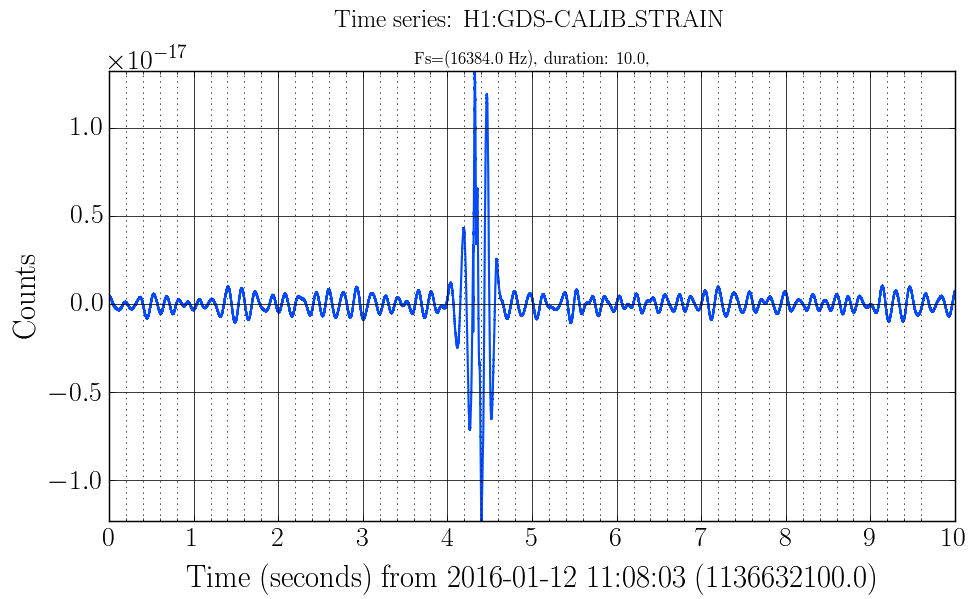
\includegraphics[width=0.495\textwidth]{figures/detchar/strain-dac-overflow}
  \label{subfig:strain-dac-overflow}
  }
\subfloat[]{
  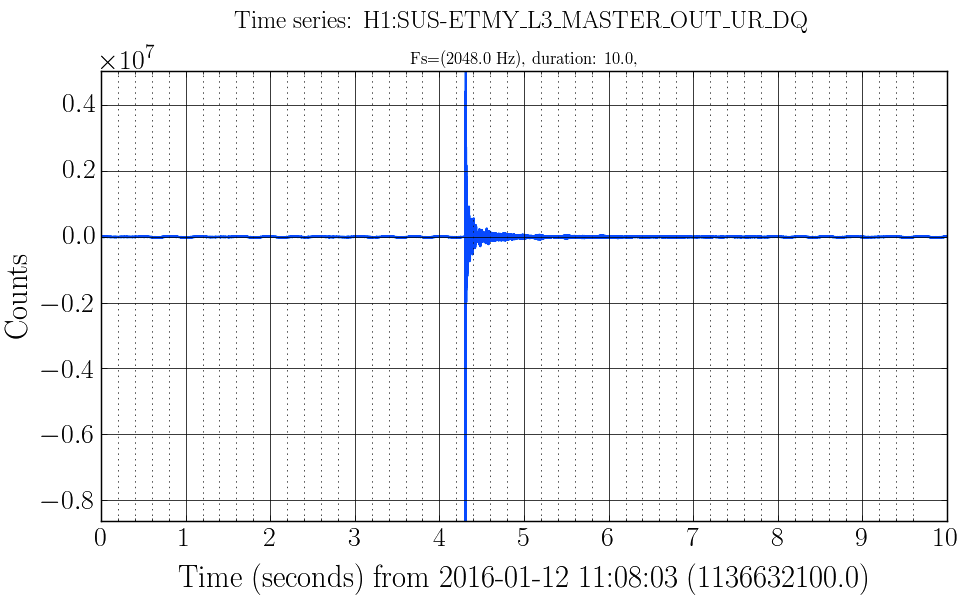
\includegraphics[width=0.495\textwidth]{figures/detchar/esd-dac-overflow}
  \label{subfig:esd-dac-overflow}
  }

\subfloat[]{
  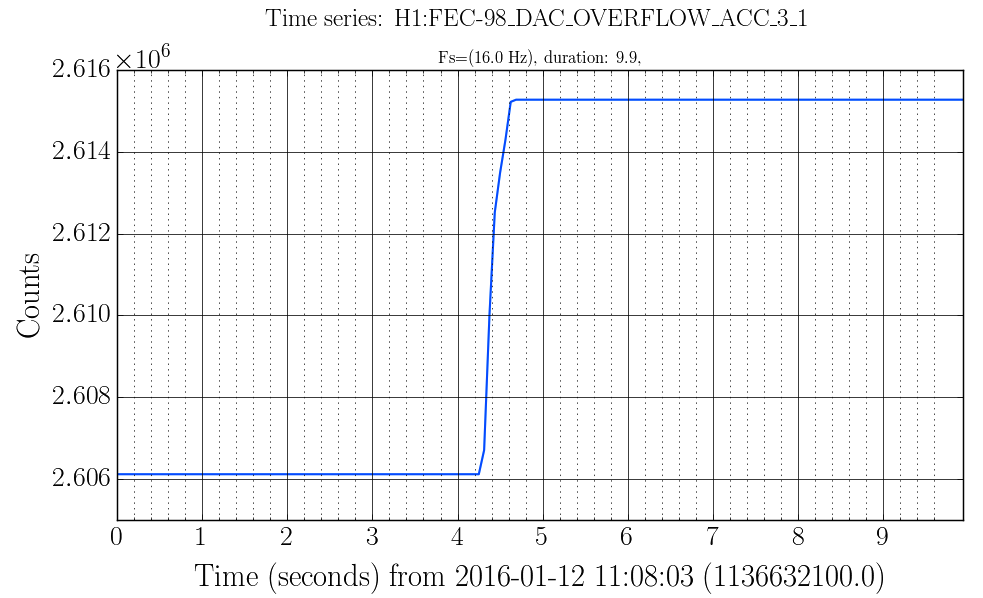
\includegraphics[width=0.495\textwidth]{figures/detchar/etmy-dac-overflow}
  \label{subfig:etmy-dac-overflow}
  }
\caption[ETMY saturation]{Timeseries of an ETMY drive signal saturation in the 
         H1 detector. Figure \ref{subfig:strain-dac-overflow} shows a glitch in 
         the calibrated $h(t)$ channel. Figure \ref{subfig:esd-dac-overflow} shows 
         the response to this glitch in the drive signal used to control the bottom 
         stage of ETMY and actuate on the DARM degree of freedom. This signal hits 
         its digital overflow point at its peak and has no more dynamic range. 
         Figure \ref{subfig:etmy-dac-overflow} shows the front end channel responsible 
         for monitoring digital overflows of this particular ETMY drive signal. 
         Since the witness channel is cumulative, overflows can be identified by 
         flagging any time in which this witness channel is increasing. }
\label{fig:dac-overflow}
\end{figure}

This method was used throughout O1 to generate data quality vetoes that 
were distributed to the Burst and CBC searches. The first veto that was 
generated this way was used to flag DAC overflows of the ETMY drive signal, 
as demonstrated 
in Figure \ref{fig:dac-overflow}. The other veto generated in this framework 
was used to flag ADC overflows in the OMC DC photodiode used as the error 
point of the DARM control loop. 

\subsection{Suspension DAC calibration glitches}

A common glitch mechanism throughout ER6 was due to calibration errors in 
digital-to-analog converters (DACs) responsible for providing analog signals 
to the aLIGO suspensions. The aLIGO suspension subsystem uses 18-bit DACs 
to interact with the optics in the interferometer. These 18-bit DACs are 
created by combining a 16-bit DAC with a 2-bit DAC inside of the same 
electronics box. The 2-bit DAC is responsible for the two highest order 
bits of the output, while the 16-bit DAC is responsible for the 16 lowest 
order bits of the output. If the 16-bit DAC and 2-bit DAC have not had 
their output voltages carefully calibrated, there will be a voltage discontinuity 
at the output of the DAC when engaging the 2 highest order bits. 

Since these DACs use the two's complement 
representation for signed binary numbers, there are two critical points 
where the two highest order bits of the DAC become necessary. The highest 
order bit is used to indicate negative numbers, so an output discontinuity 
is expected when transitioning from a positive number to a negative number, 
that is, crossing through a value of zero.  
The other bit from the 2-bit DAC is used to represent large output values and 
engages when the DAC needs to express a value which is unable to be 
represented by a 16-bit DAC alone. As such, we also 
expect to see discontinuities when the DAC output crosses $\pm2^{16}$. 

The fact that this discontinuity existed in suspension subsystem was 
particularly problematic, as the suspension DACs are used to directly 
actuate on mirror positions and optical cavity lengths. Any time a 
suspension DAC crossed one of these problematic output values, it would 
actuate on the optics with a step function and cause a glitch in the 
optical cavity length. Figure \ref{fig:DAC-glitch} shows an example of 
this issue where the DAC providing actuation signals to the power recycling 
mirror (PRM) is crossing through zero and there are associated glitches 
visible in the length readout of the power recycling cavity.

\begin{figure}[ht!]%
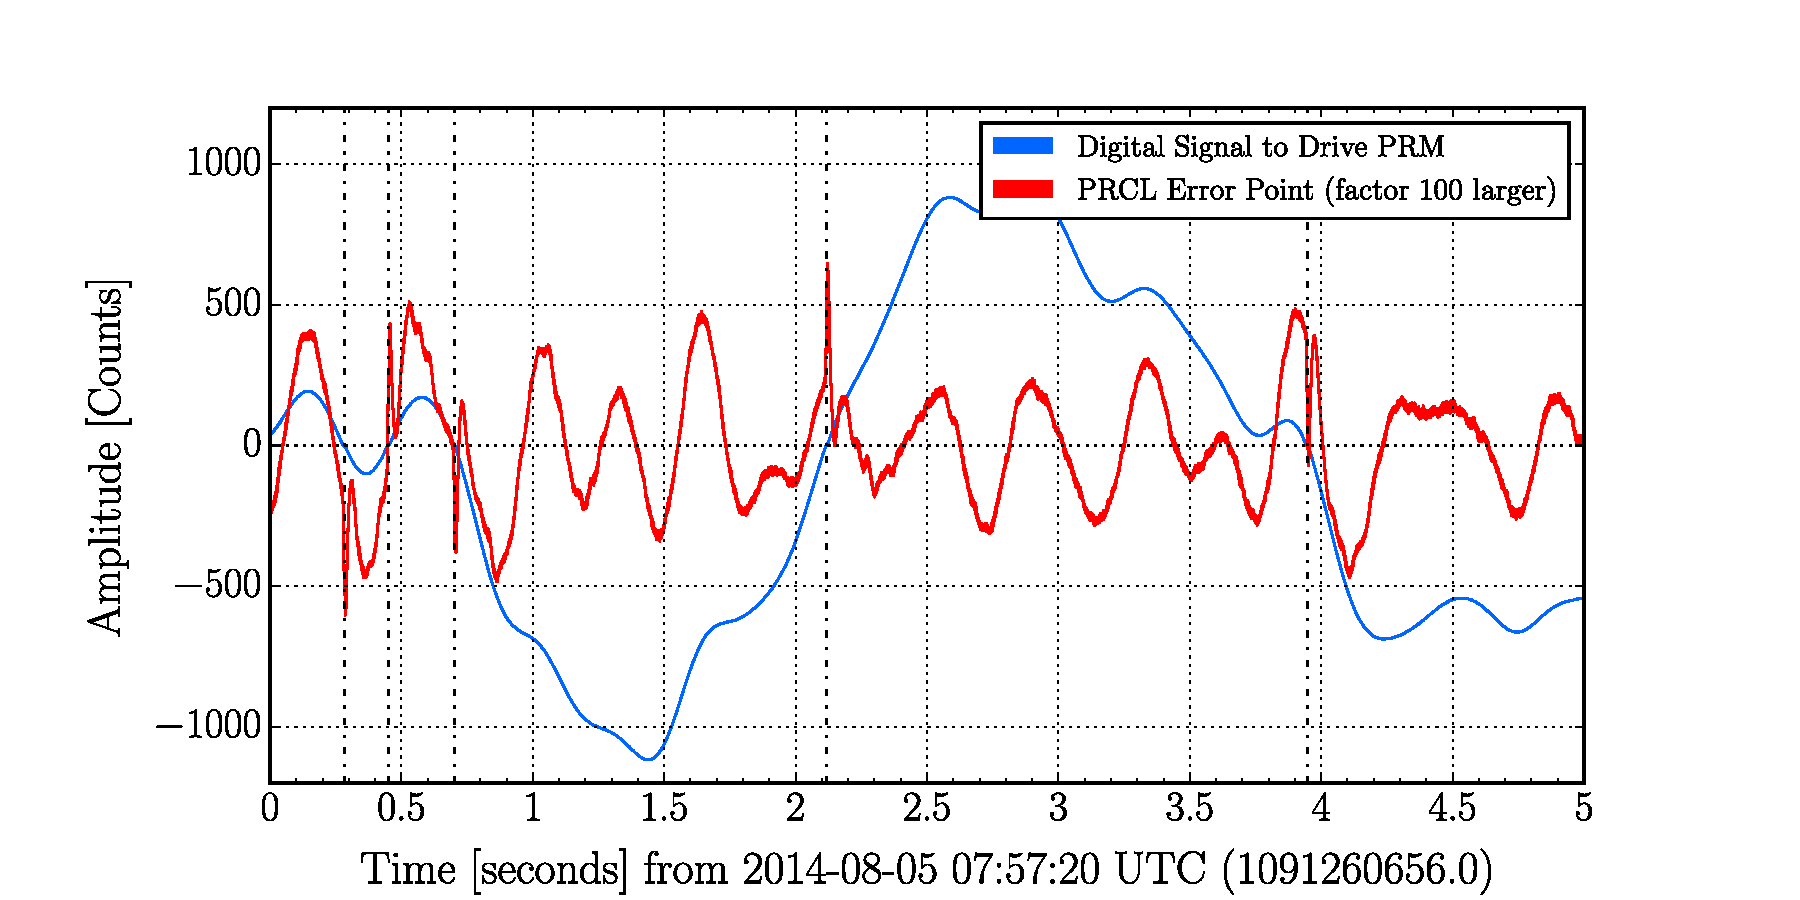
\includegraphics[width=\textwidth]{figures/detchar/PRCL-DAC-glitch}
\caption[DAC glitches in PRCL]{A timeseries plot showing the effects of %
         DAC calibration glitches. The red trace shows the digital drive %
         signal being sent to the digital-to-analog converter. The blue %
         shows the resulting power recycling cavity motion rescaled by a %
         factor of 100. When the drive signal crosses %
         through a value of zero, the output of the DAC experiences a %
         discontinuity, leading to a glitch in the power recycling cavity %
         length.}
\label{fig:DAC-glitch}
\end{figure}

The effects of this issue were visible in the $h(t)$ channel during ER6. 
The most problematic culprit was the DAC that applied actuation directly 
to the optics of the ETMs, effectively pushing directly on the DARM degree 
of freedom and causing glitches in $h(t)$. These calibration errors manifested 
themselves as a population of glitches in $h(t)$ recovered by Omicron in the 
20-100 Hz range. This is a very damaging frequency range for CBC searches, 
which hope to accumulate significant SNR in the region from 30-500 Hz.  
This population of low frequency glitches was obvious in an Omicron 
time-frequency scatter plot and was considered a significant noise source 
throughout the sixth engineering run.

Figure \ref{fig:vetoed-DAC} shows the result of an Hveto run that looked 
for time correlations between Omicron triggers in $h(t)$ and times when 
the ETMY drive signal crossed through a value of $2^{16}$. The blue dots 
represent all Omicron triggers in $h(t)$. The red crosses indicate those 
that were coincident with the ETMY drive signal crossing $2^16$. The 
population of low frequency glitches with SNR $>$ 8 was shown to be 
coincident with the drive signal transitions. This veto 
was very statistically significant, as shown in Table \ref{table:etmy-dac-hveto}. 
The significance 
of 192.5 indicates that the probability of these coincidences being due 
to noise alone is negligible. The effiency:deadtime ratio of 27 indicates 
that these glitches were removed with very small time windows (0.2s) 
and very little instrument uptime was removed in the process.

\begin{figure}[ht!]%
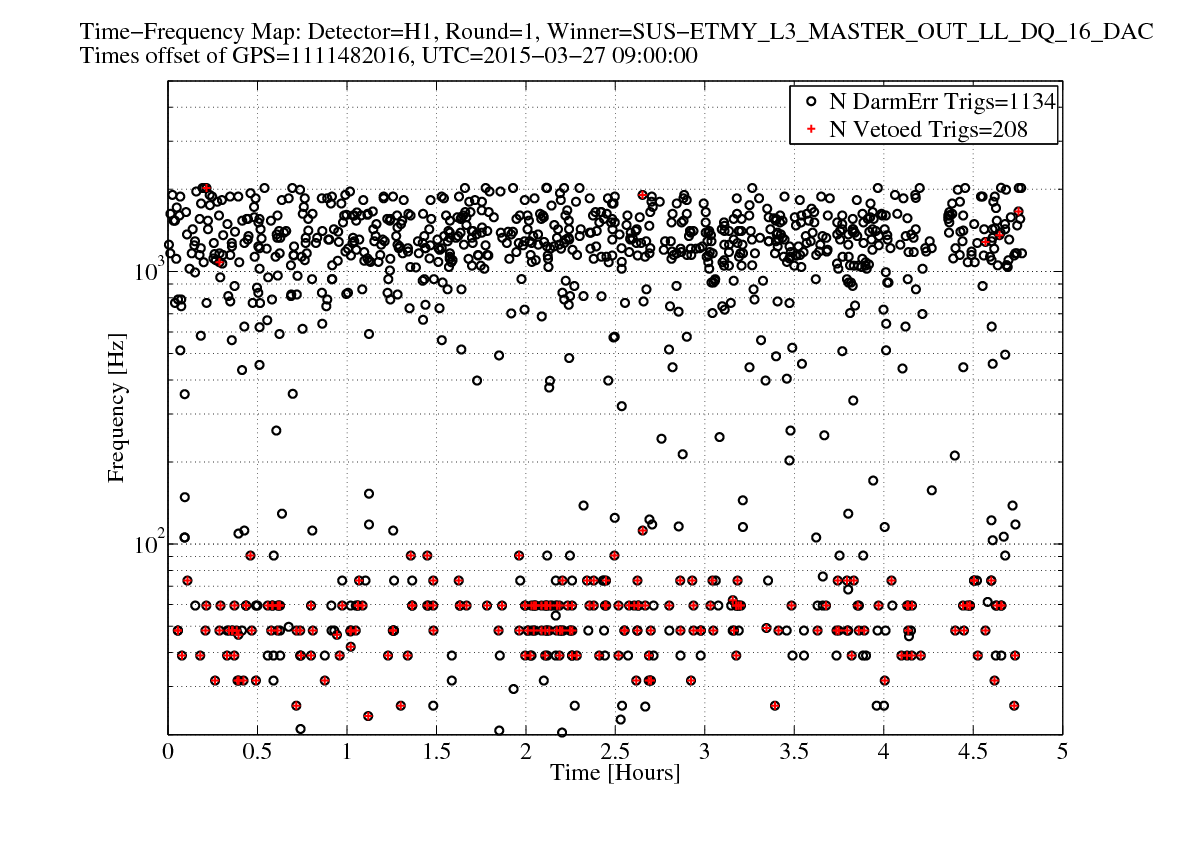
\includegraphics[width=\textwidth]{figures/detchar/vetoed-DAC-glitches}
\caption[Vetoed DARM triggers from DAC calibration]{A time-frequency %
         visualization of Omicron triggers in the H1 $h(t)$ channel. % 
         The black circles indicate glitches in the DARM degree of freedom, %
         each with a central time and central frequency. The red crosses %
         indicate that a given trigger was vetoed by an auxiliary channel %
         trigger which was found to be statistically significant using Hveto. The %
         auxiliary channel triggers in this case indicate that the drive signal %
         on the bottom stage of ETMY has crossed a value of $2^{16}$. The %
         population of glitches between 20 - 100 Hz is highly coincident %
         with these crossings of $2^{16}$, indicating that they are caused %
         by DAC calibration errors on this optic.}
\label{fig:vetoed-DAC}
\end{figure}

\begin{table}[ht!]%
 \footnotesize 
 \begin{center}
  \begin{tabular}{cccccc}
  \hline
  Channel & \begin{tabular}{@{}c@{}} Time \\ window (s) \end{tabular} & 
            \begin{tabular}{@{}c@{}}SNR \\threshold \end{tabular} & 
            Significance & Efficiency \% & Deadtime \% \\ 
  \hline
  \begin{tabular}{@{}c@{}}ETMY drive signal \\ crosses $2^{16}$ \end{tabular} & 
  0.2 & 8 & 192.5 & 18.3 &  0.674 \\
  \hline
  \end{tabular}
  \end{center}
  \caption[HVeto results for ETMY DAC glitches]{Hveto results for ETMY DAC glitches}
  \label{table:etmy-dac-hveto}
\end{table}

To fully understand the scope of this problem, the Detector Characterization 
group developed software that searched through the output of all suspension 
DAC digital output signals and marked times when they crossed 0 or $\pm2^{16}$. 
These marked times were converted into trigger files and sent through Hveto 
to look for correlations between crossings of critical values and glitches 
in DARM as identified by Omicron. Through this method, we were able to identify 
which optics were experiencing DAC calibration glitches that had a coupling 
mechanism into DARM.

There were two approaches taken in an effort to mitigate these DAC glitches. The 
first was to introduce offsets into the suspension drive signals so that they 
did not cross through a value of zero. This did solve the problem temporarily, 
but at the cost of a significant portion of the dynamic range of the output 
actuation. The more permanent fix was to run a calibration routine 
that resolved the issue between the 16-bit and 2-bit DACs. This was 
successful, though it had to be run on a weekly basis during site maintenance 
because the calibration tended to drift away from its nominal point after 
2-3 weeks of operation.

During the first observing run, the systematic check of all suspension DAC 
digital output signals was performed again and the resulting triggers were 
sent through Hveto. This study revealed that the calibration process was 
successful; there was no evidence of residual DAC calibration glitches that 
had any noticeable coupling into $h(t)$. The only signal that had any 
significant correlation with glitches in $h(t)$ was not causally sensible. 
Large glitches $h(t)$ were driving the ETMX actuation signal through a value of 
$2^{16}$, which resulted in crossings of $2^{16}$ that were coincident in time 
with glitches in $h(t)$, but weren't representative of calibration errors.

\textcolor{red}{Discuss Hveto results}

\subsection{RF beatnote whistles}

Two RF oscillators beating against one another creates a kHz beatnote that couples 
into DARM.

\begin{figure}[ht!]%
\centering
\subfloat[]{
  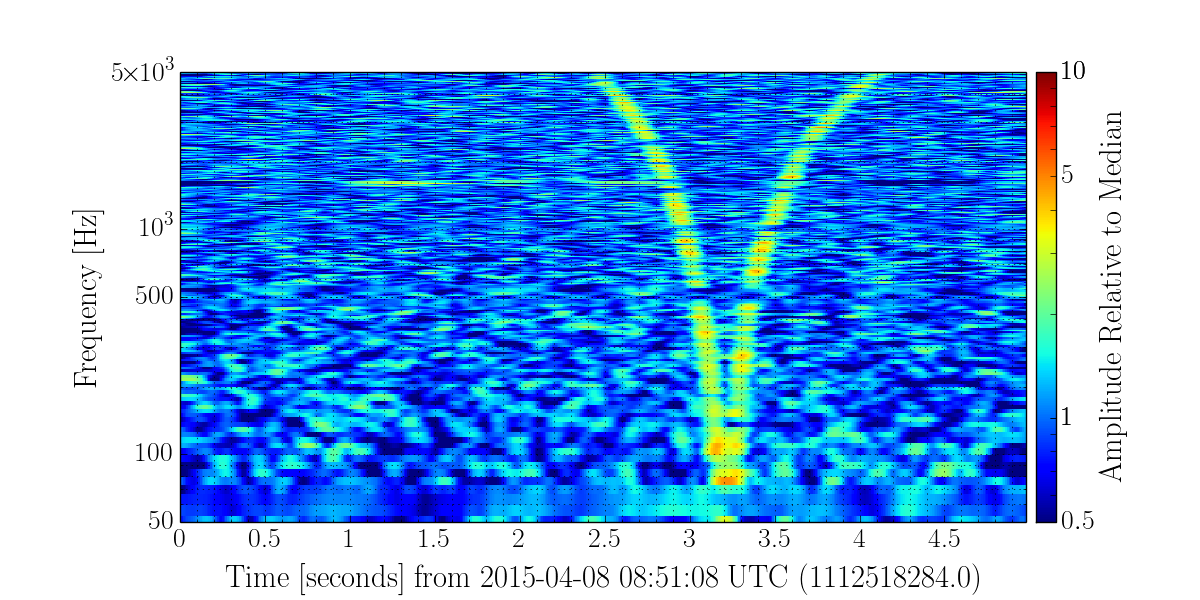
\includegraphics[width=\textwidth]{figures/detchar/Spectrogram_Whistle_LLO}
  \label{subfig:llo-whistle}
  }
  
\subfloat[]{
  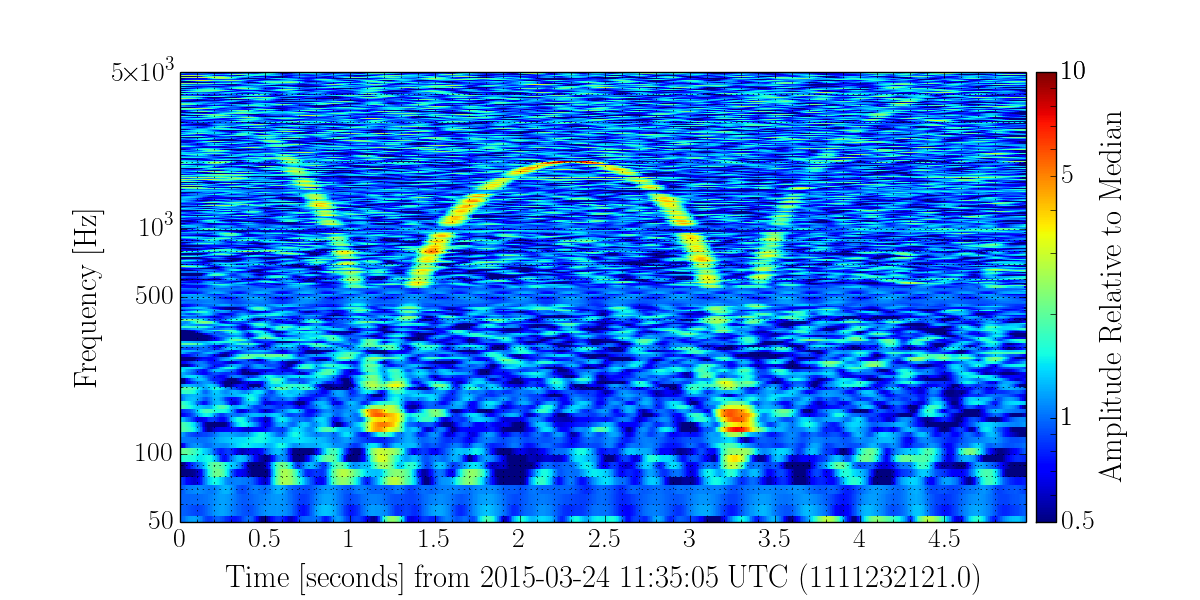
\includegraphics[width=\textwidth]{figures/detchar/Spectrogram_Whistle_LHO}
  \label{subfig:lho-whistle}
  }
\caption[Spectrograms of RF whistles]{Time-frequency spectrograms of RF whistles at %
         both LLO and LHO. Figure \ref{subfig:llo-whistle} shows a %
         whistle at LLO sweeping down from the kHz range and into the detection band %
         where it interferes with searches for gravitational waves. Figure %
         \ref{subfig:lho-whistle} shows a double whistle whistle at LHO where the %
         two oscillators drifted back and forth across one another and caused two %
         glitches in the detection band.}
\end{figure}\label{fig:whistle-spectrograms}

Hveto shows that a witness channel for RF whistles vetoes approximately 90\% 
of DARM triggers in this time period.

\begin{figure}[ht!]%
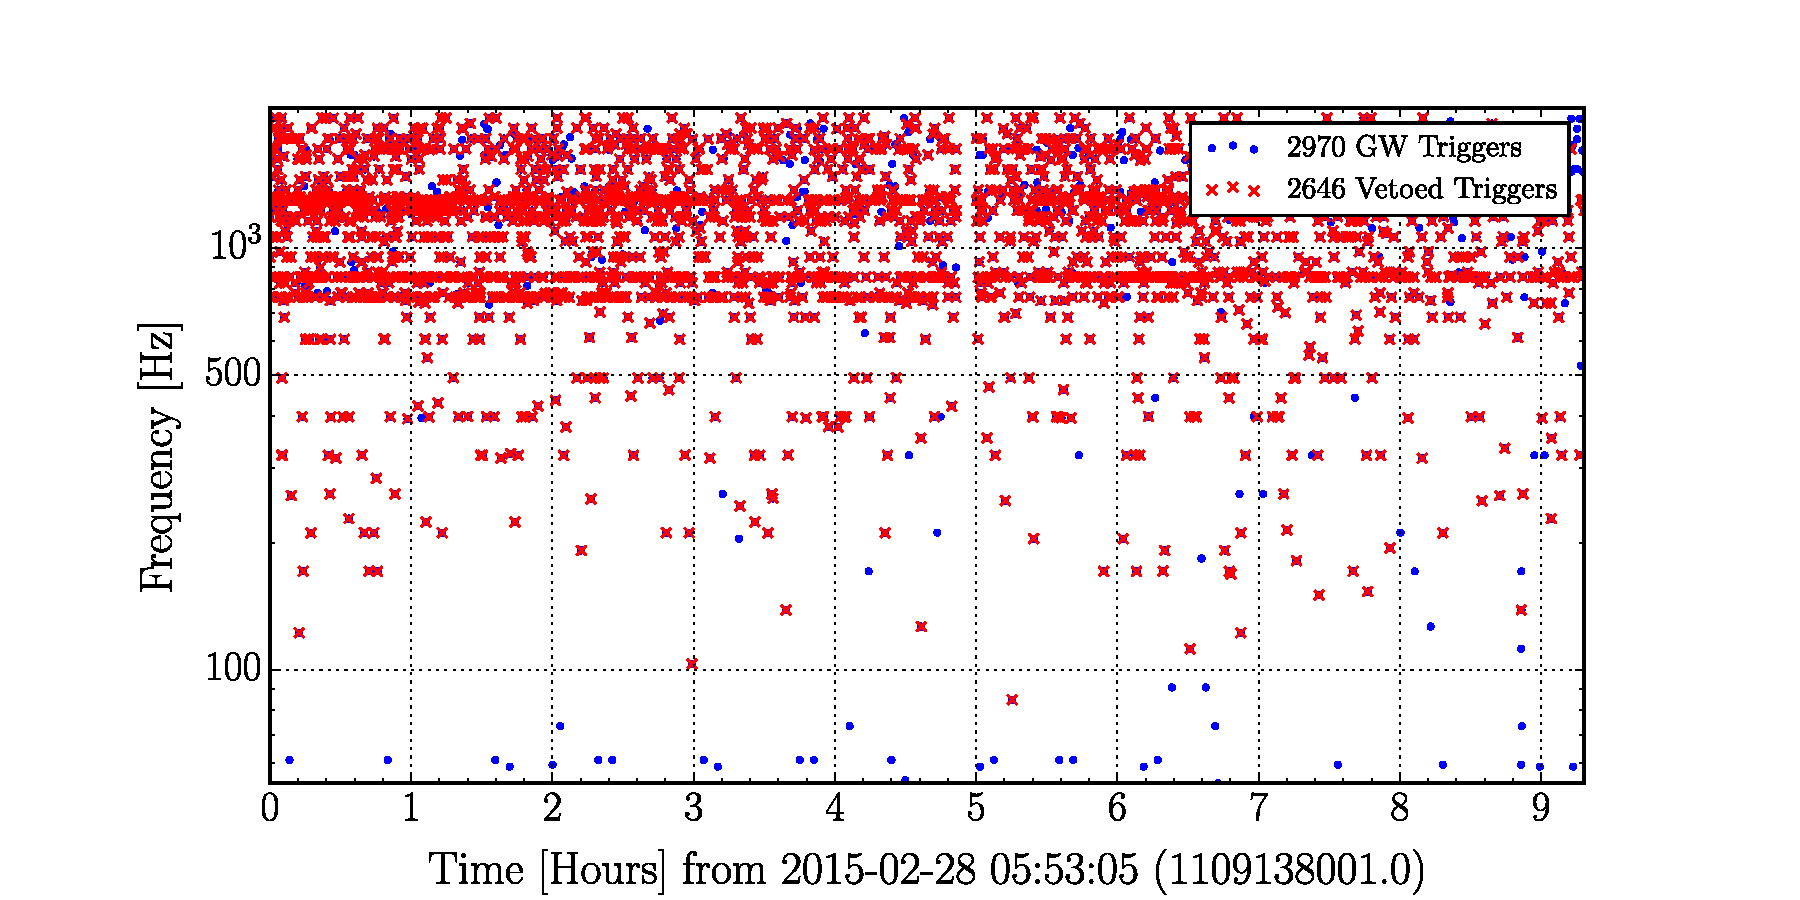
\includegraphics[width=\textwidth]{figures/detchar/Hveto_whistles_time_frequency}
\caption[Vetoed whistles from Hveto]{A time-frequency scatter plot of $h(t)$ Omicron %
         triggers. The blue dots represent all triggers found for the $h(t)$ channel. %
         Red crosses indicate that a trigger was determined to be coincident with an %
         RF whistle and vetoed. This veto is responsible for removing 90\% of the %
         glitches in this time period. The majority of the high frequency glitches %
         were due to RF beatnote whistles}
\end{figure}\label{fig:hveto-whistles}

How do we know that the frequency offset worked? Look at a signal that is a proxy 
for the drifting oscillator and histogram all of the Omicron DARM triggers during 
that time. If there's no coupling, the answer should be fairly Gaussian; the 
IFO is just as likely to glitch at any value of the channel. If there are 
channel values that correspond strongly to glitches in DARM, we should see peaks.

\begin{figure}[ht!]%
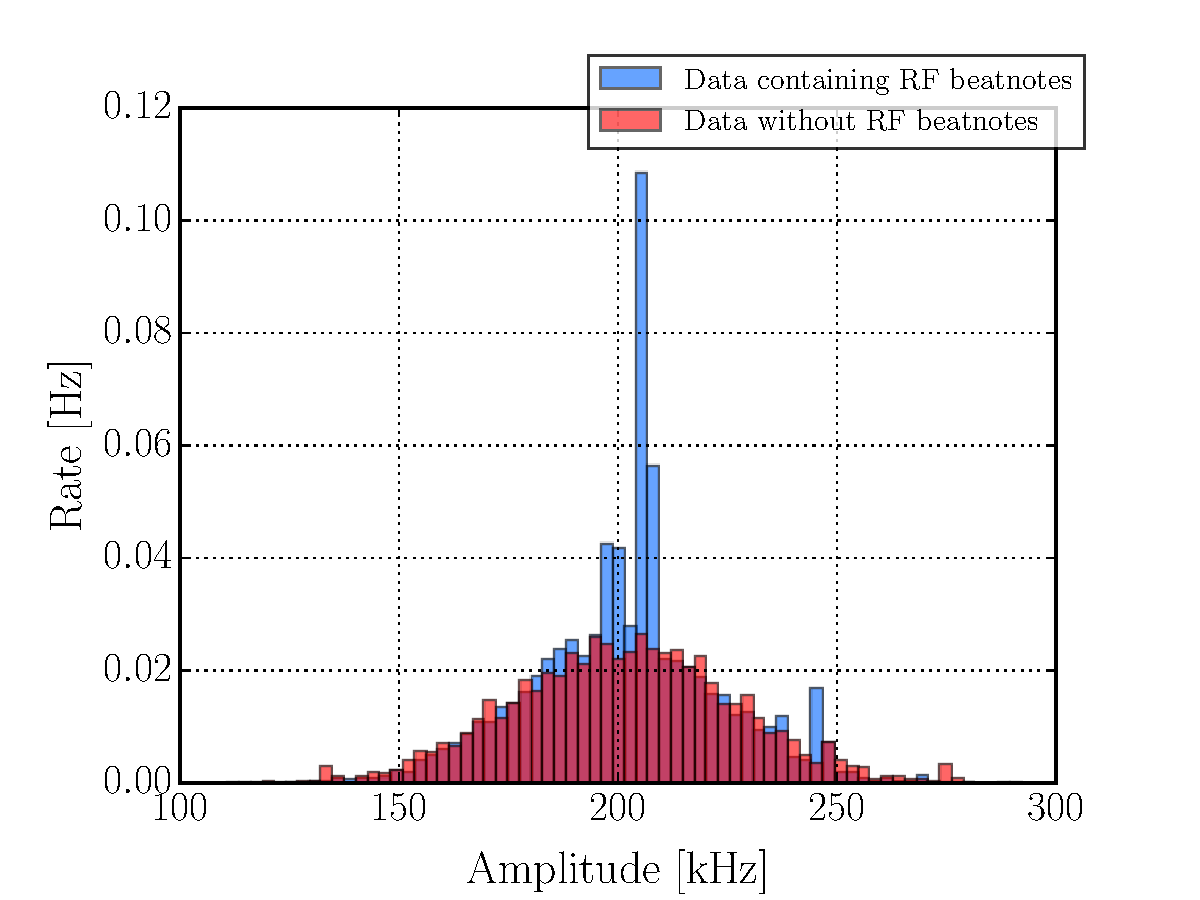
\includegraphics[width=\textwidth]{figures/detchar/Rate_Histogram_Whistles_LLO}
\caption[DARM glitch histograms with and without RF whistles]{Red curve is nice %
         and Gaussian. Blue curve has peaks that indicate problematic frequencies.}
\end{figure}\label{fig:darm-whistle-hist}

\subsection{Seismic CPS comb}

Oscillators in the capacitive position sensors had drifted apart and caused a 
beatnote and a comb. Audio analysis pointed towards amplitude modulation. 

Fixed by slaving all oscillators to a master.

\subsection{DC values of auxiliary channels}

No great correlation at the end of the day 

\subsection{Earthquakes during full lock}

Lots of scattering arches during an earthquake, drove up the noise and biased PSD.
Caused a sarlacc, removing this data was able to repair data on either side.

\subsection{L1 PMC glitches}


Characterization of noise and analysis after repair

\subsection{Data quality shifts}
Performed and mentored data quality shifts.





\Chapter{IMC Upconversion}
\label{ch:IMCUpconversion}
\section{Abstract}

LIGO interferometers use several high finesse optical cavities for gravitational wave detection. The lengths of these cavities are controlled using radio frequency (RF) modulation-demodulation techniques in a Pound-Drever-Hall (PDH) locking scheme. This scheme provides a PDH error signal that is linear to cavity length over a specific range. This study examines the specific case of the triangular ring cavity uses in LIGO interferometers for input mode cleaning. When the length of the cavity approaches the boundaries of the PDH error signal linear range, our model of the input mode cleaner PDH response shows that the resulting error signal contains non-linear spectral artifacts. This model and understanding of the non-linear cavity responses will be useful in the commissioning phase of the Advanced LIGO project for more precisely locating and eliminating systematic noise sources in the interfereometers

\section{Model}

The PDH response of the cavity was modeled using measured values of optical reflectivity and free spectral range of the Livingston input mode cleaner. The input beam was the nominal LIGO carrier beam with a frequency of $\omega = 281.8$ THz ($\lambda = 1064$ nm) and modulation sidebands of $\Omega = \pm24$ MHz.

The reflection coefficient of a LIGO input mode cleaner as a function of input beam frequency is given as,

\begin{equation}
F(\omega) = \frac{r(1 + e^{-i\phi})}{1+r^2e^{-i\phi}} = \frac{r(1 + e^{-i(\frac{\omega}{\nu_{fsr}})})}{1+r^2e^{-i(\frac{\omega}{\nu_{fsr}})}}
\end{equation}

where $r$ is the reflectivity of the input mirror, $\phi$ is the round-trip phase accumulated when traversing the cavity, and $\nu_{fsr}$ is the free spectral range of the cavity \cite{Mueller}.

In a situation where the carrier beam is resonant in the cavity and the modulation sidebands are high enough in frequency that they are not resonant, the PDH error signal, here denoted $\epsilon$ is given as

\begin{equation}
\epsilon(\omega) = -2\sqrt{P_{c}P_{s}}\operatorname{Im}\{F(\omega)F^*(\omega + \Omega) - F^*(\omega)F(\omega - \Omega)\},
\end{equation}

where $P_{c}$ is the the carrier beam power and $P_{s}$ is the sideband power \cite{Black01}.

Note: the above error signal is a function of laser frequency. This is an artifact of the original intent of PDH locking: using a fixed length resonant cavity to control the frequency of a laser by forcing it to match the cavity length. We can apply the same technique but flip the direction of feedback and use a highly stable laser to control the length of a free swinging resonant cavity by pushing on the mirrors to match the cavity length to the laser wavelength. The laser frequency detuning and cavity length detuning are linearly mapped to one another using the free spectral range of the resonant cavity.

Importantly, this error signal is linear to the length of the IMC within a certain range of motion. If the optics begin swinging too far away from the nominal locking point, we will begin to see a non-linear response and eventually a lock loss.

To explore this non-linearity, we injected a sinusoidal cavity motion into our model and observed the resulting error signal.

We explored two specific cases. Figure 1 shows spectra of the injected sinusoidal cavity motion (green) and the resulting non-linear error signal (blue). This motion was injected asymetrically about the nominal cavity locking point ($\epsilon = 0$) and therefore we see both even and odd harmonics of the injection frequency.

Figure 2 shows spectra of the injected sinusoidal cavity motion (green) and the resulting non-linear error signal (blue). However, this time the motion was injected symetrically about the nominal cavity locking point and as a result we only see odd harmonics of the fundamental frequency.

We hope to use this model as an explanation of systematic noise found in the aLIGO IMC.

\begin{figure}[h!]
\caption{Sinusoidal cavity motion with frequency 2.78 Hz injected asymmetrically about the locking point of the cavity results in a PDH error signal containing non-linear spectral artifacts at harmonics of the injected cavity motion.}
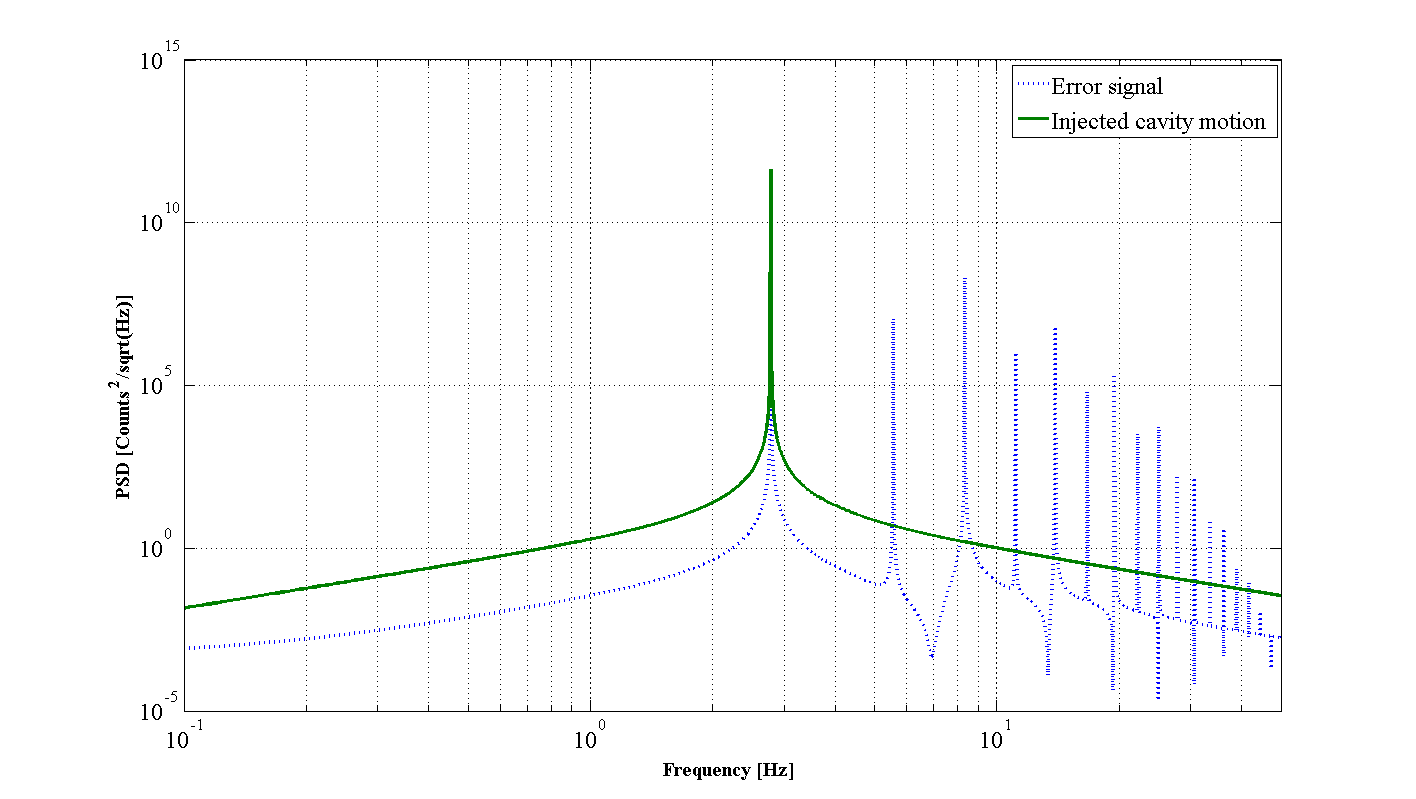
\includegraphics[height=0.6\textwidth]{figures/IMCUpconversion/PDH_error_signal_harmonics.png}
\end{figure}

\begin{figure}[h!]
\caption{If the motion is symmetric about the cavity locking point, we see only odd harmonics of the injection frequency.}
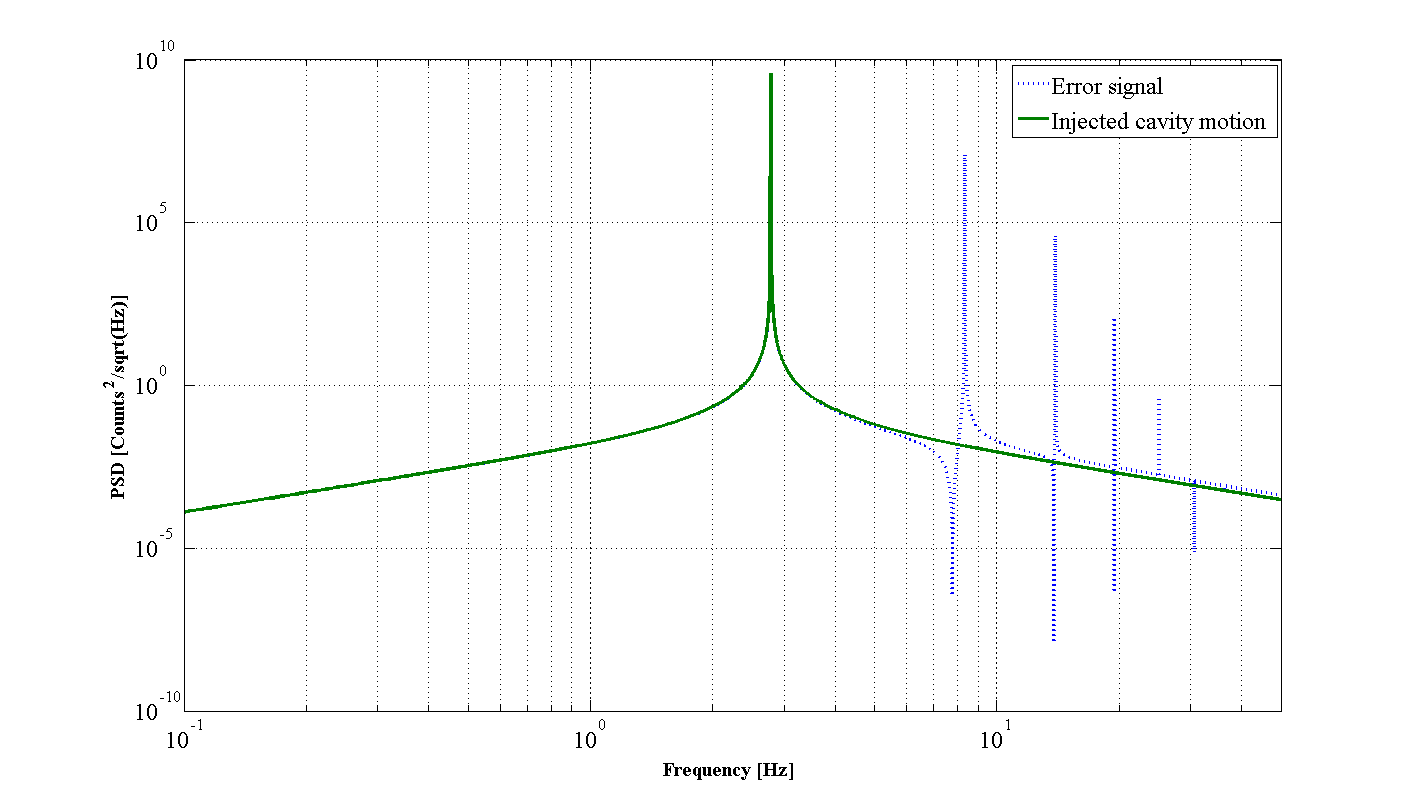
\includegraphics[height=0.6\textwidth]{figures/IMCUpconversion/symmetric_PDH.png}
\end{figure}

\section{Upconversion noise in aLIGO}
The aLIGO input mode cleaner (IMC) is a triangular ring cavity whose length is sensed and controlled using the PDH locking technique. Each of the three mirrors in the cavity is staged as the bottom mass of a triple suspension in order to passively isolate the mirrors from  potential noise sources. In addition, the chambers holding the IMC mirrors are isolated from ground motion by two stages of active seismic isolation. This isolation, however, is not completely impervious to external excitations. During periods of time with excess ground motion we can see seismic noise coupling into the cavity length and its control signal.

Specifically, when we see excess seismic noise in the 1-5 Hz anthropogenic band (believed to be caused by a commercial railroad a few kilometers from the LIGO Livingston Laboratory), we see highly structured noise in the IMC control signal in the 10-100 Hz band. This physical mechanism is consistent with the idea of a PDH range saturation. If excess seismic motion reaches the suspension and the optics begin swinging around, it's feasible that they could start to saturate the linear range of the PDH loop.

The noise takes a form very similar in structure to the non-linear PDH signal, displaying strong odd harmonics and weaker even harmonics. The IMC control signal has an associated noise floor that obscures parts of these peaks. The theoretical model uses sinusoids with a highly specified frequency and thus displays very sharp peaks in its spectrum. It should be noted that the peaks in the IMC control signal are the manifestation of a physical process, not digitally generated, and have some natural width to them.

\begin{figure}[h!]
\caption{Spectral comb with a fundamental frequncy of 2.78 Hz in the IMC control signal. Red arrows indicate odd harmonics, green arrows indicate even harmonics. }
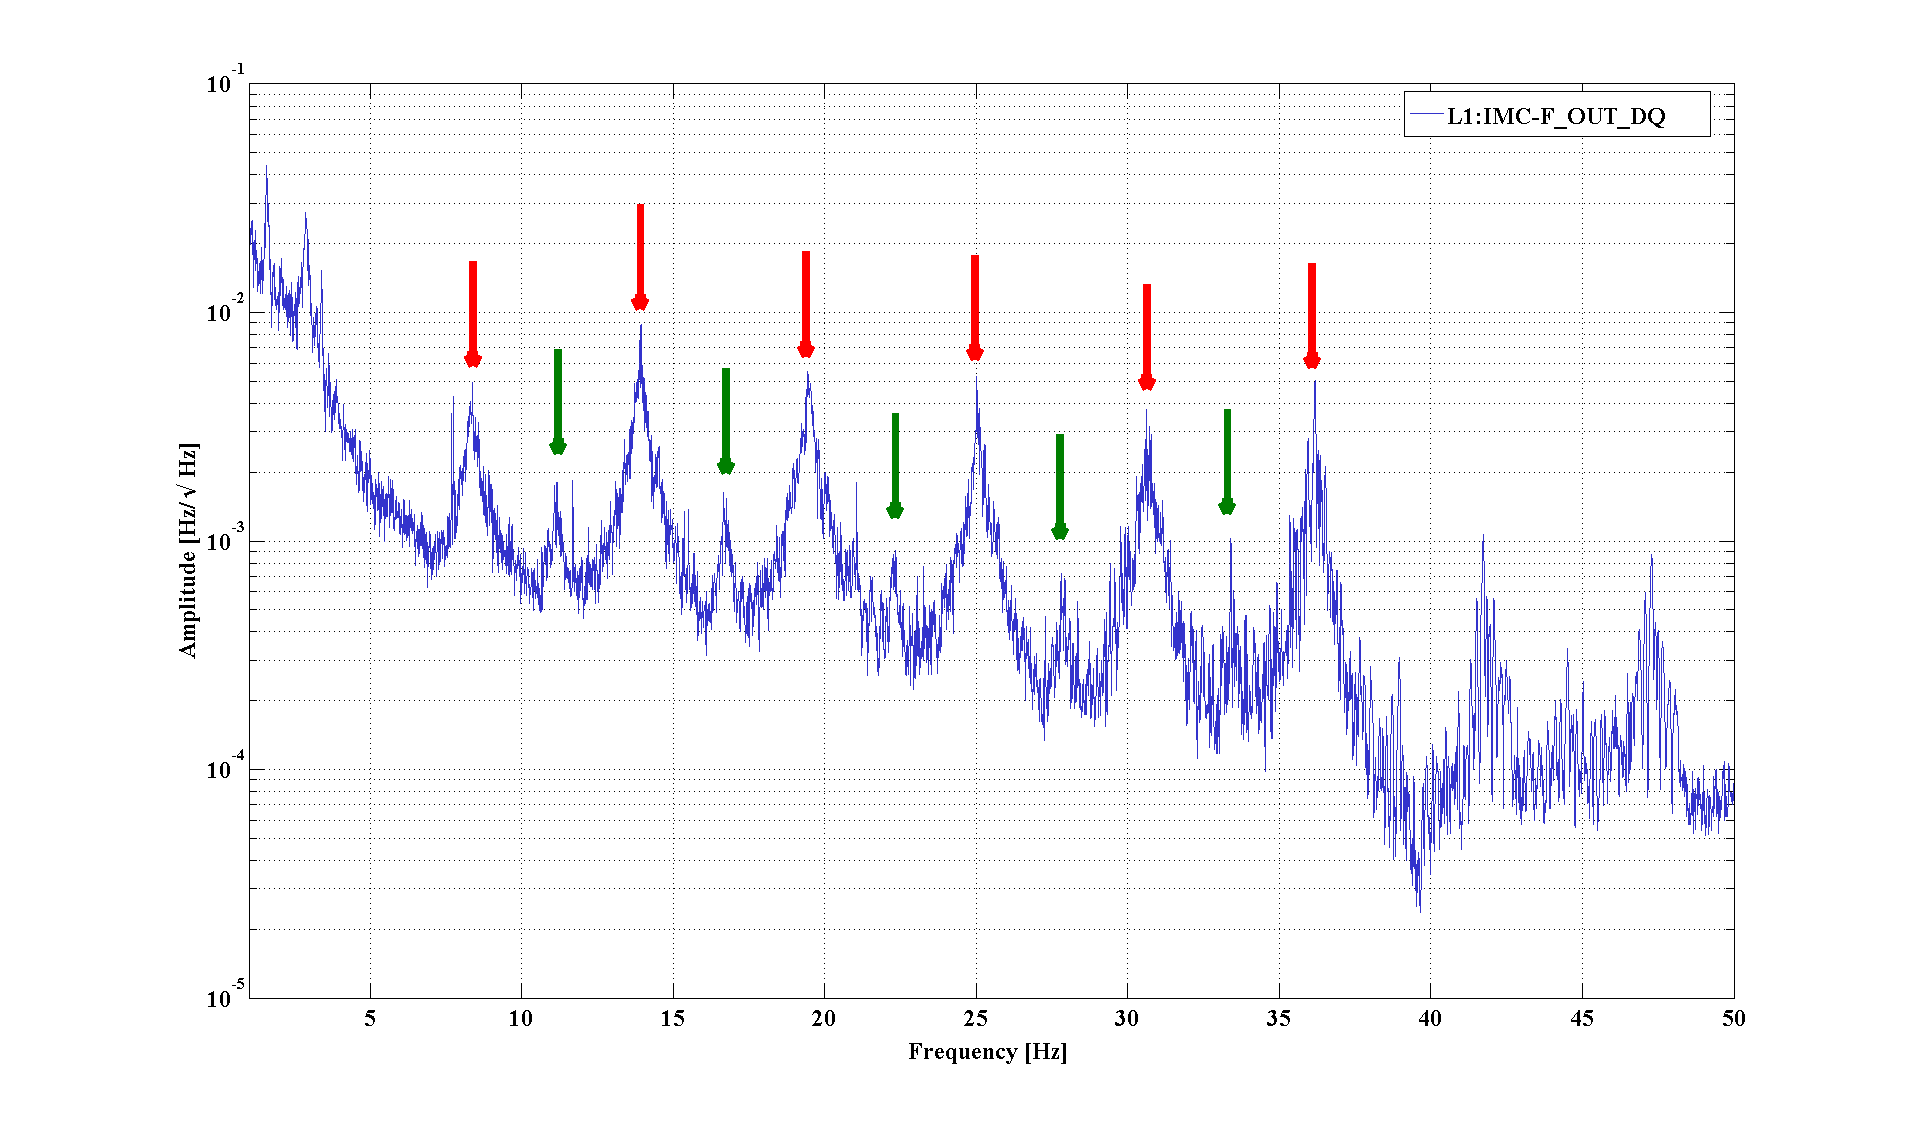
\includegraphics[height=0.6\textwidth]{figures/IMCUpconversion/upconversion_comb.png}
\end{figure}

\section{Next steps}

While we have demonstrated that this mechanism is a feasible explanation for the IMC upconversion noise, it has not yet been fully proven. We are currently looking for a better way to look at the actual IMC error point during times of excess seismic motion instead of the control signal. 

We also need to localize the source of the 2.78 Hz excitation. Why that specific frequency when the excess seismic noise is spread across a 1 - 5 Hz band? We think the source may be a vertical resonance of the triple pendulum suspension that houses the IMC optics being rung up by the excess motion.

We are also going to use the increasing full IFO uptime to figure out whether or not this upconversion noise is coupling downstream into critical cavities such as the recycling or arm cavities.

\section{Conclusions}

We found that injecting sinusoidal cavity motion into our input mode cleaner PDH model generates an error signal with non-linear spectral artifacts, specifically harmonics of the injection frequency, if the cavity motion exceeds the linear PDH range. For cavity motion that is symmetric about the locking point of the error signal, we find that the error signal contains only odd harmonics. For asymmetric cavity motion we find both even and odd harmonics, where the odd harmonics are typically higher in amplitude. In such a case, the amplitude of the even harmonics increases as the DC offset from the nominal locking point increases, that is, as the cavity motion is more asymmetric.



\Chapter{Detector Characterization Subsystem Lead}
\label{ch:ODC}
The aLIGO interferometers are highly complex, high precision devices. 
Their operation depends on the careful interaction of a series of subsystems, 
each with its own purpose. In an effort to better understand the operation 
and output of the interferometers, the Detector Characterization group has 
been designed to mirror this subsystem approach. Table 
\ref{table:aligo-subsystems} lists the aLIGO subsystems. Each of these 
subsystems is assigned a data quality liaison from the DetChar group. 

\begin{table}[ht!]%
  \begin{center}
    \begin{tabular}{|c|l|}
    \hline
    Subsystem & Description \\
    \hline
    LSC & Length Sensing and Control \\
    \hline
    ASC & Alignment Sensing and Control \\
    \hline 
    SUS & Suspensions \\
    \hline
    IMC & Input Mode Cleaner \\
    \hline 
    OMC & Output Mode Cleaner \\
    \hline
    PCAL & Photometric Calibration \\
    \hline 
    PEM & Physical Environmental Monitoring \\
    \hline
    SEI & Seismic Isolation \\
    \hline
    PSL & Pre-Stabilized Laser \\
    \hline
    TCS & Thermal Compensation System \\
    \hline
    \end{tabular}
  \end{center}
  \caption[Table of aLIGO subsytems]{Table describing aLIGO subsystems}
  \label{table:aligo-subsystems}
\end{table}

There are 5 main responsibilities assigned to a subsystem liaison. The 
first is to fully understand the operation and installation of the subsystem 
so that they can faciliate data quality investigations and act as a 
point of contact for commissioners assigned to this subsystem.

The second responsibility 
is to take this knowledge and use it to populate the channel information 
system (CIS), which is a database that stores information about how to 
parse and understand the various auxiliary channels that are monitored 
in each subsystem. This database also contains information about calibration 
and valid frequency ranges for these channels. This allows newcomers to the 
collaboration to more easily familiarize themselves with the LIGO naming 
conventions and facilitates their involvement in data quality investigations.  

The third responsibility 
is to check for signal fidelity, which means to make sure that all of the 
channels are working as intended and don't contain artifacts from signal 
conditioning processes.

The fourth responsibility is to develop summary pages that monitor 
important channels and figures of merit for each subsystem. 
The summary pages are generated 
every day from a configuration file designed by the subsystem liaisons. 
The purpose of the summary pages is to gather all of the potentially 
useful information about a subsystem in an organized way so that the 
subsystem leads can efficiently evaluate the performance of the subsystem. 
They are also a useful launch point for data quality shifts and 
investigations since they provide various overviews of instrumental 
performance ($h(t)$ spectrograms, Omicron triggers, BNS inspiral range, etc.) 
that make it easy to identify persistent or egregious data quality issues.

The fifth and final responsibility is to develop and build real-time 
data quality monitors in the Online Detector Characterization (ODC) 
framework. 
The Online Detector Characterization (ODC) system is an infrastructure designed
to extract and record metadata describing the state of the aLIGO interferometers.
This state information has two main purposes: to inform data quality investigations
by the DetChar group and to serve as a real-time monitor of the interferometer state
that can be accessed in the control room. Each subsystem monitored by the DetChar group
using an ODC monitor.

The ODC system is unique in that it is runs in real-time in the front-end control
system that is used to control the aLIGO interferometers. Each set of ODC monitors
is built in Simulink to directly interface with the models that run on the front-end
computers. This has several distinct advantages.
Since the monitors are run in real-time, they operate in parallel with the control
loops that are sensing the various degrees of freedom of the interferometer and are
able to achieve highly precise timing. The ODC monitors can also create their own
test points, which means an ODC monitor can perform a check on any signal that exists
in the front end at its full rate instead of relying on the information that is
downsampled and stored in frames.
These full rate test points operate at the full sample rate of the model (16384 Hz)
and any information recorded in the ODC channel is written at the same rate. In contrast,
many channels are only recorded at 16 Hz if they aren't accessed as a test point in the front-end system.

The information generated by each ODC monitor can be extracted and sent to a segment
generation process, where the most useful information is catalogued and represented by
segments of time that indicate when a given flag was considered to be active.

\section{Length Sensing and Control}

The Length Sensing and Control (LSC) subsystem is 
used to monitor and control the lengths of the various optical cavities in the 
aLIGO interferometers. Figure (insert) shows the layout 
of the aLIGO interferometer with the lengths of individual optical cavities 
labeled. The LSC subsystem is responsible for controlling 5 global degrees of freedom, 
which are linear combinations of these individual cavity lengths. Table (insert) 
describes the primary degrees of freedom controlled by the LSC subsystem. 
This is a critical subsystem, as it is used to control
not only the auxiliary optical cavities, but the DARM degree of freedom which
is sensitive to gravitational wave signals.
These optical cavities are controlled using the Pound-Drever-Hall (PDH) 
technique described in Section ?? .

\subsection{Online Detector Characterization}

The ODC model for the LSC subsystem is designed to monitor the feedback 
loops used to control optical cavities. A series of test points are placed 
in the control loop and compared to user-set threshold values to determine 
whether or not they are in their nominal range. 
Figure \ref{fig:lsc-odc-model} shows the implementation of an LSC ODC 
model in SIMULINK. The numbered ovals on the left of the image are test point 
signals that are being read in from the higher level model that is used to control the 
lengths of the optical cavities. The signals are carried along the wires connecting 
each box. The green boxes are where the user set thresholds are saved. The white 
boxes perform operations on input signals.

As an example, we'll follow the path of inputs 46 and 47, which are signals from 
the photodiode that measures the reflected light at the input to the power recycling 
cavity. The signals are read in at the ovals labelled 46 and 47, their absolute values 
are calculated at the boxes labeled 'Abs19' and 'Abs20'. The absolute values of these 
signals are then fed into boolean comparison boxes, 'Operator39' and 'Operator40'. 
These boolean operator boxes are also connected to the green box which defines a 
threshold for the signals to be compared to. If the input signals are less than the 
designated threshold, the boolean operator passes a value of True. If they have 
exceeded the intended threshold, the boolean operator passes a value of False. 
The outputs of the two boolean operators are fed into one last check, which performs 
an AND operation. If both signals have passed their tests and reported True, the AND 
block reports a True and this photodiode signal is considered to be in a good state. 
If one or both of the signals has failed their test, the AND block reports a False 
and the photodiode signal is considered to be in a bad state. This answer is stored 
as a bit in the ODC state vector for the LSC subsystem. 

Some of the checks implemented in the ODC models are more complicated. For 
example, when 
the states of multiple control loops are stored in a vector they can be compared to a 
series of state masks that select which degrees of freedom to check. 
In this way, the same vector of information used to perform hierarchical 
checks on the state of the instrument. 
One test can check that the core optics are performing nominally, a more broad 
test can include checks on both the core optics and recycling cavities, and 
then the overall test can be done to check that feedback loops are performing as intended. 
Each of these tests will report its own answer that is stored in the ODC state vector.

\begin{figure}[ht!]
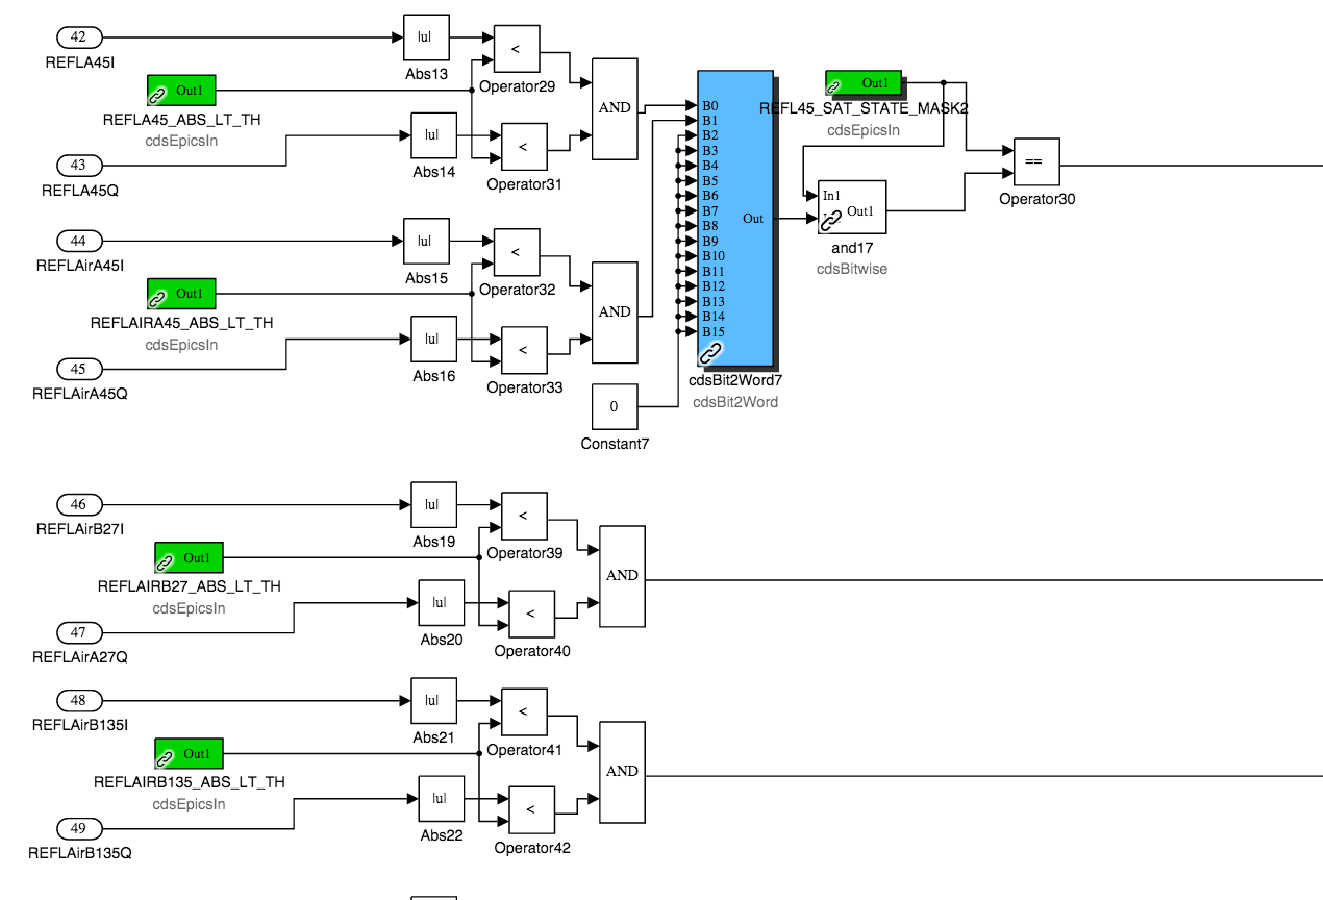
\includegraphics[width=\textwidth]{figures/ODC/LSC-ODC-model}
\caption[LSC ODC SIMULINK Model Example]{LSC ODC checks implemented in SIMULINK. %
         The numbered ovals on the left indicate signals used in real-time control %
         of the interferometer. The green boxes represent user-defined threshold %
         values to be used in boolean comparisons. The white boxes represent operations %
         such as computing the absolute value of a signal or performing boolean %
         comparisons (less than, greater than, AND, OR, etc.)}
\end{figure}\label{fig:lsc-odc-model}

Once the ODC model has performed all of its checks and reported a True or False 
answer, the information is stored in an overall state vector that can be parsed to 
learn the state of the LSC subsystem at any time. 
Figure \ref{fig:lsc-odc-bits} shows a visual representation of the state of the 
length degrees of freedom in the H1 interferometer over the course of a day.
Each horizontal bar represents the state of a length degree of freedom as 
reported by ODC. In this particular day, the control signals for the Michelson 
(MICH) and signal recycling cavity (SRCL) degrees of freedom exceeded their 
nominal range while the interferometer was in its nominal operating state. 
This is indicated by the color of the bars switching between 6:00 - 8:00 UTC 
and between 14:00 - 16:00 UTC. All of the times when the state changes are 
recorded as time segments which can be used to correlate excursions in the 
cavity control signals with transients in the output of the interferometer. 

\begin{figure}[ht!]
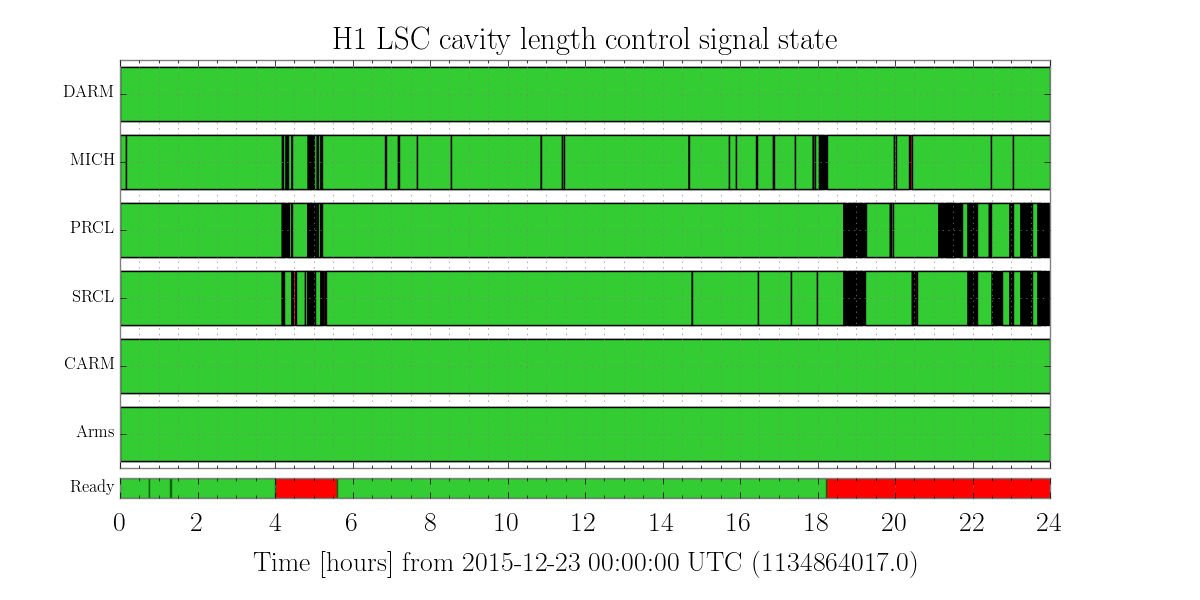
\includegraphics[width=\textwidth]{figures/ODC/LSC-bit-example}
\caption[LSC ODC bits example]{ODC bits representing states of length degrees of %
         freedom. Each horizontal bar represents a length degree of freedom that %
         is controlled in the LSC subsystem. When the bar is green, the control %
         signal for that degree of freedom is in its nominal range. When the %
         bar is not green, the control signal for that particular length degree %
         of freedom has exceeded the threshold set in the ODC model and is reported %
         as out of range.}
\label{fig:lsc-odc-bits}
\end{figure}

\subsection{MEDM screens}

For real-time use of these monitors, a software package called MEDM is used to 
display and interact with the ODC models. MEDM can be used to update the thresholds 
and state masks used to determine the status of a given photodiode or degree of 
freedom. 
Figure \ref{fig:lsc-odc} shows the LSC ODC overview screen in MEDM. 
The top panel summarizes the overall state of the subsystem, showing the state of 
each ODC bit and a bitmask that indicates whether or not a given bit is used in 
determining the overall state of the subsystem. 
The leftmost 
panel is used to monitor the state of each length degree of freedom in the interferometer. 
The rest of the panels are used to monitor the states of the various photodiodes used 
for sensing length degrees of freedom. These include DC power monitors and the values 
of RF demodulated photodiode signals. The grey boxes containing numerical values indicate 
user-set thresholds that can be updated from this screen.

\begin{figure}[ht!]
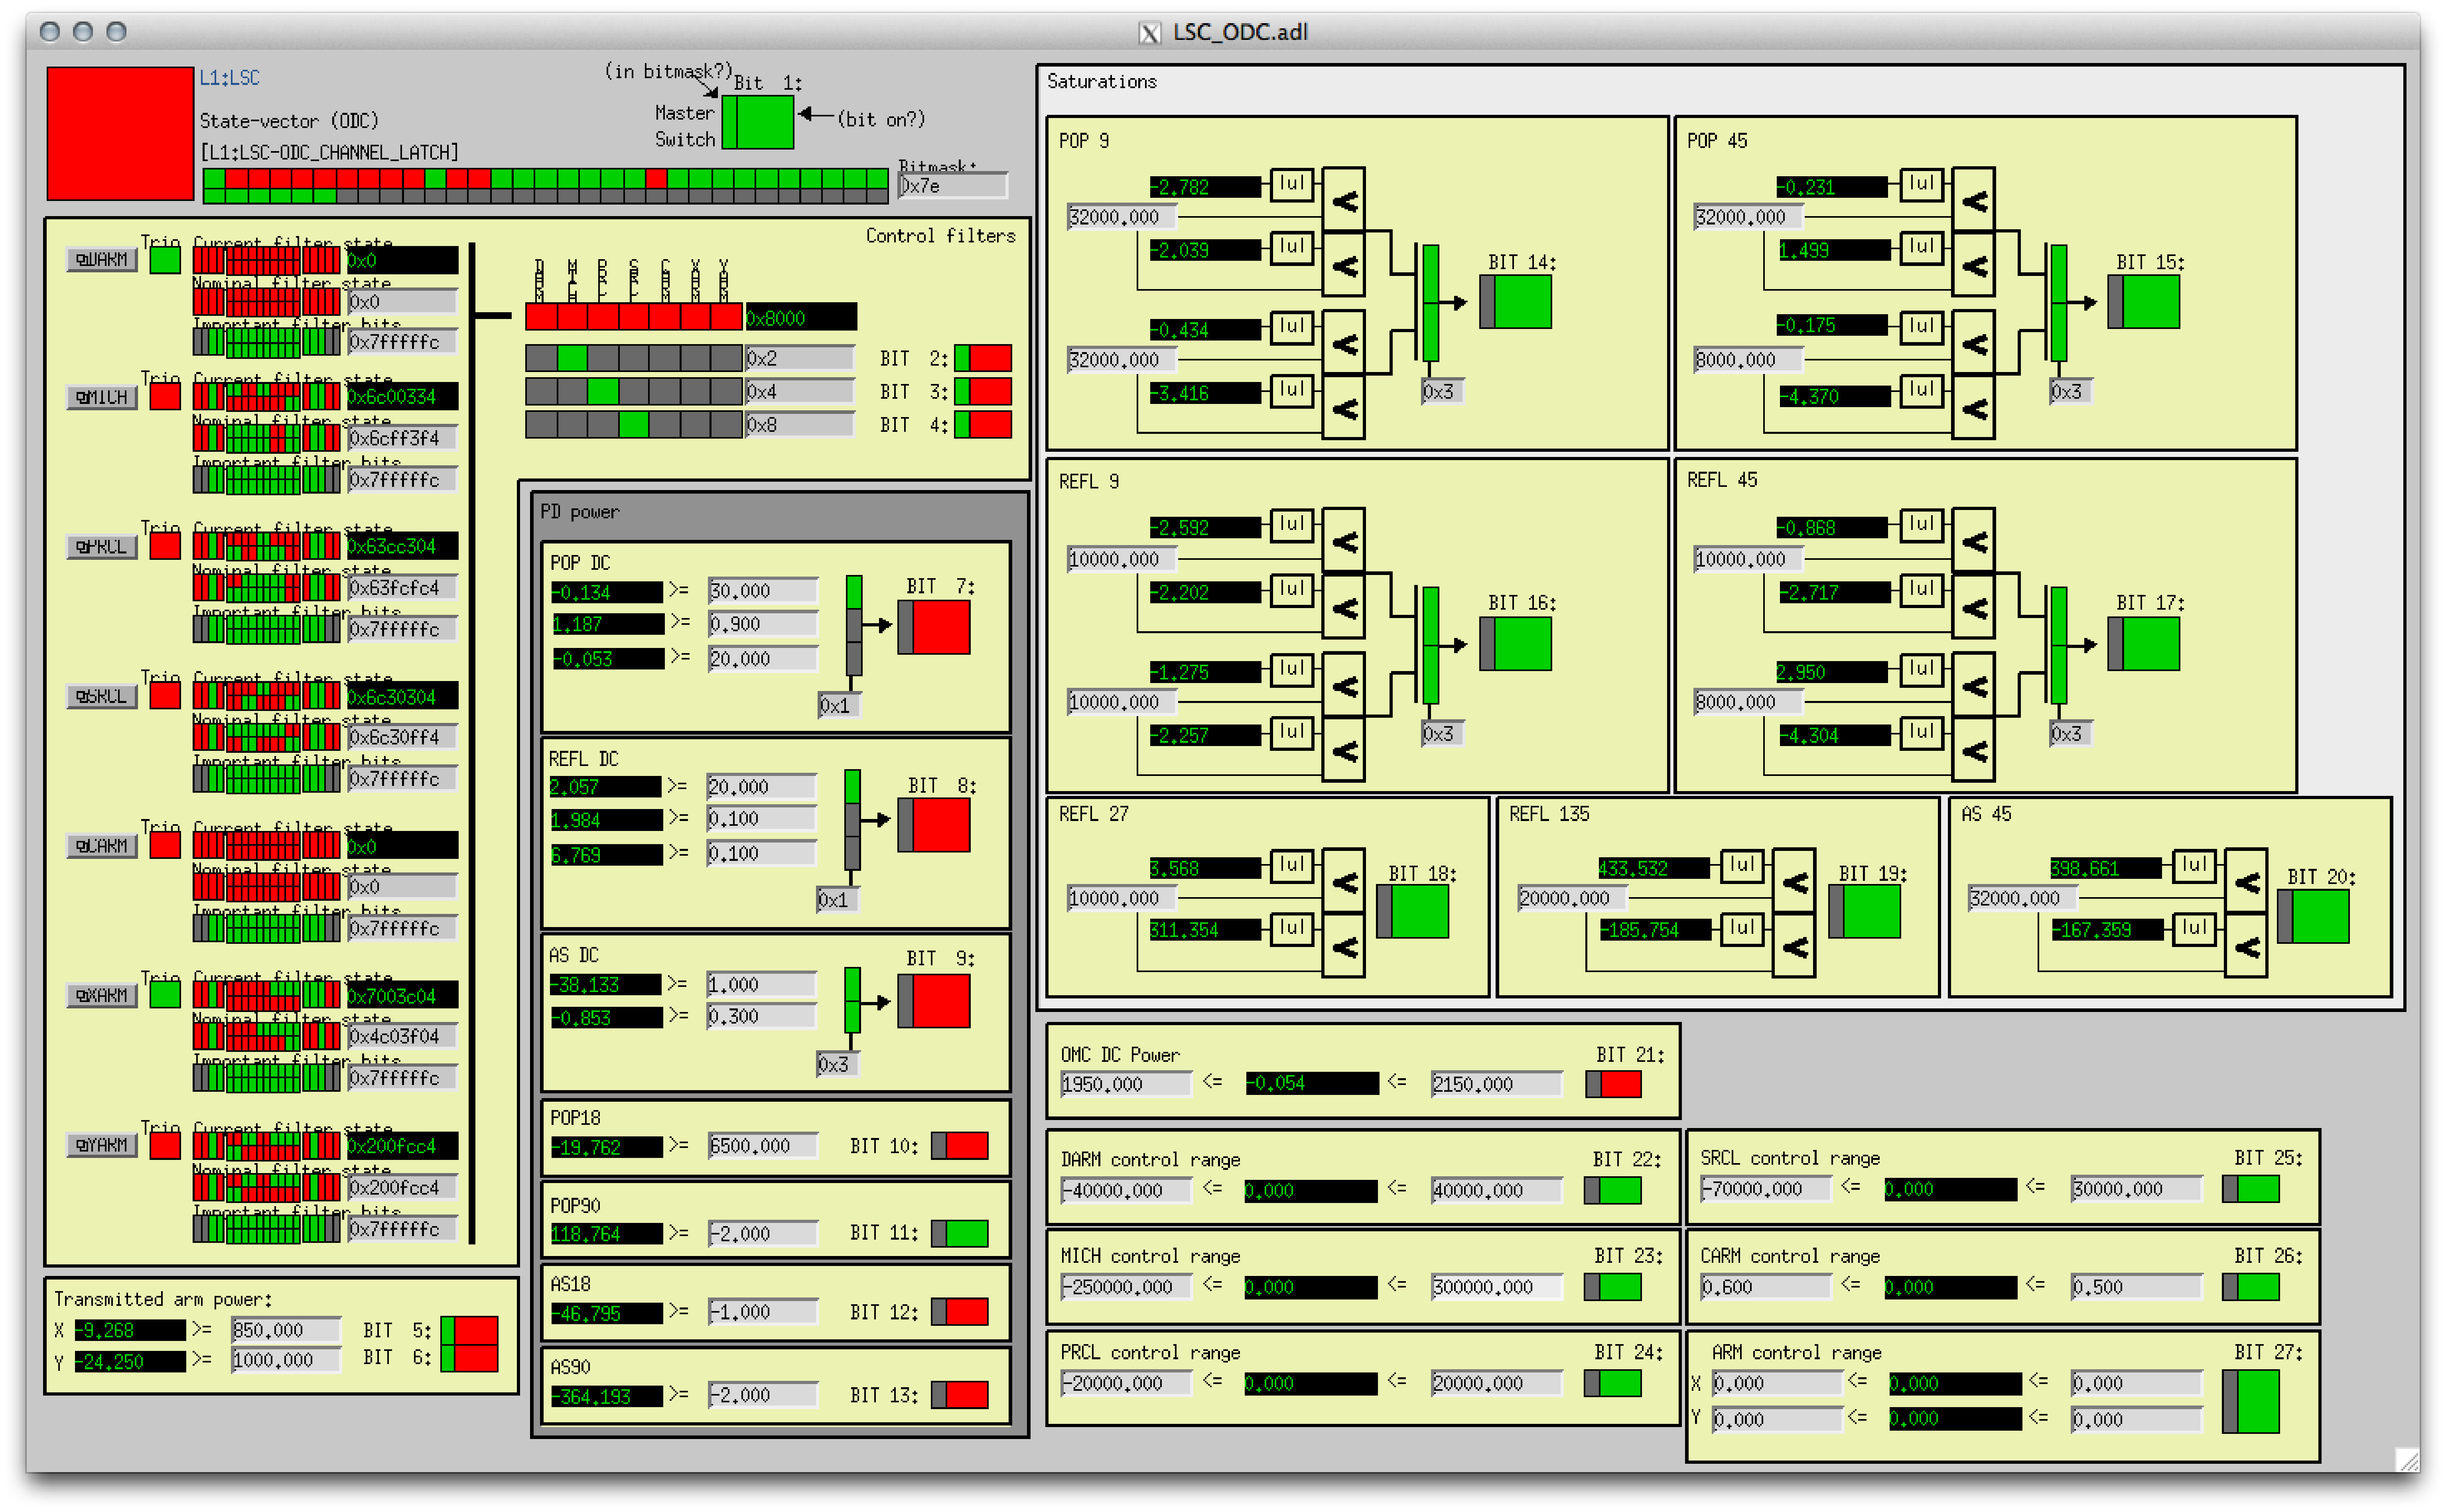
\includegraphics[width=\textwidth]{figures/ODC/LSC_screen}
\caption[LSC ODC Overview Screen]{MEDM screen used to interact with the LSC ODC model. %
         This screen contains information regarding the overall state of the LSC subsystem, %
         the state of control loops pertaining to specific length degrees of freedom in the %
         interferometer, and the state of photodiodes used to sense length degrees of freedom %
         in the interferometer.}
\label{fig:lsc-odc}
\end{figure}

\subsection{Summary pages}

While the MEDM screens are useful for real-time readout of the ODC models, they do not 
have an easily accessible history. For this reason, summary pages were built that 
contain the most important information from each ODC model. The summary pages are 
built multiple times per day and are accessible through a web browser, which allows 
easy, organized access to past interferometer data when performing a data 
quality investigation. 

Figure \ref{fig:lsc-odc-bits}, which shows the status of the length degrees of freedom 
of the interferomter over the course of a day, was taken from the summary pages. In this 
figure, the MICH degree of freedom was seen to move into a bad state during a locked state. 
As an example, we can look at the summary page visualization of the MICH degree of freedom 
during this time. 
Figure \ref{fig:mich-summary-pages} shows the control signal for the MICH degree of freedom 
with the ODC threshold 
overlaid as a dashed red line. The solid blue line indicates the median value of this signal 
over the course of 1 minute and the shaded regions indiate the maximum and minimum over 
this same stretch of time. When the control signal exceeds the ODC threshold, such as at 
about 14:35 UTC, the corresponding bit in Figure \ref{fig:lsc-odc-bits} flashes red to 
indicate the excess noise in this channel. 

\begin{figure}[ht!]
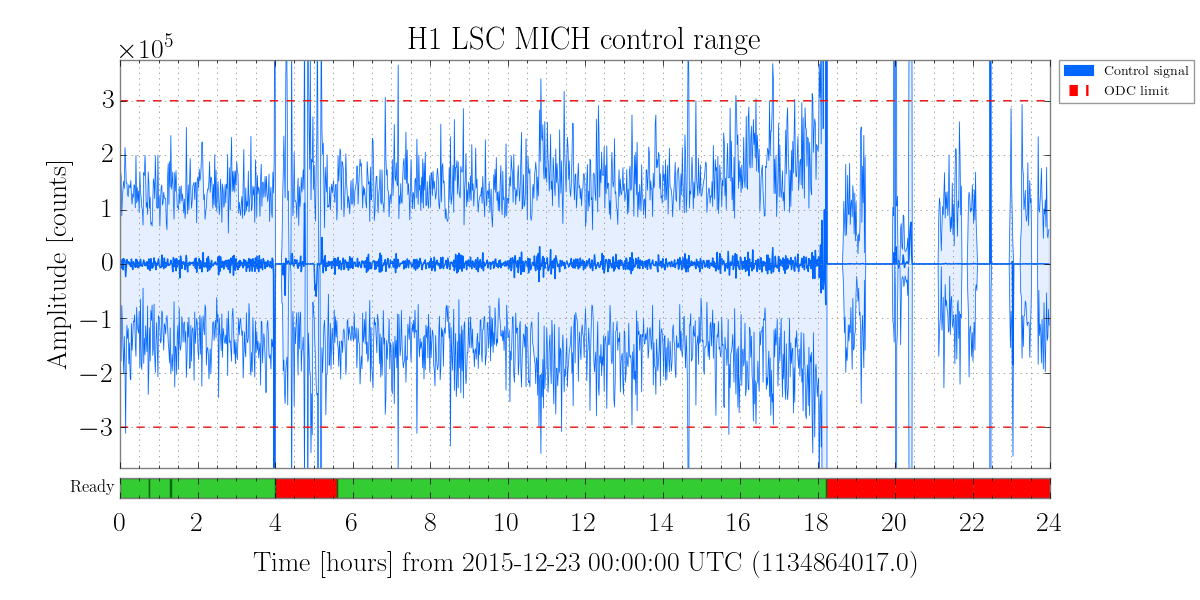
\includegraphics[width=\textwidth]{figures/ODC/H1-MICH-SUMMARY-PAGES}
\caption[MICH control signal on summary pages]{Readout of the MICH degree of freedom as %
         displayed on the summary pages. The dark blue curve indicates the median value of %
         the MICH control signal over the course of 1 minute. The shaded regions indicate %
         the maximum and minimum values of the control signal over the same stretch of time. %
         The dashed red line indicates the ODC threshold set to monitor this control signal.}
\label{fig:mich-summary-pages}
\end{figure}

\section{Alignment Sensing and Control}

The alignment sensing and control subsystem is used to control the alignment of 
optical cavities as well as the input pointing of light into those cavities. 
The control loops work in a similar way as the length sensing and control subsystem, 
using the reflected light from optical cavities to control the optics in a PDH 
scheme. The same set of RF sidebands that are used for length control are also used 
for alignment control. The detail that allows length fluctuations to be decoupled from 
alignment fluctuations is that alignment fluctuations generate higher order 
modes in the optical field, which are used in the demodulation stage to 
generate an error signal.

A length control loop compares the TEM00 mode of the carrier beam to the TEM00 
mode of the RF sidebands. 
An alignment control loop will compare the TEM00 mode of the carrier 
beam with the TEM10 and TEM01 modes of its sidebands, which are generated by 
angular misalignments of optical cavities. 
Since each optic has two alignment degrees of freedom that are directly 
controlled, pitch and yaw, and each cavity is comprised of multiple optics, 
the reflected light from each cavity is read out on a 
pair of quadrant photodiodes. This is visualized in Figure \ref{fig:odc-pd-screen}. 
The four quadrants allow the pitch and yaw error 
signals to be decoupled. Since higher order optical modes have a different Gouy 
phase as they propagate through space, a pair of photodiodes separated by a Gouy 
phase telescope are used to determine the origin of the misalignment 
(cite Nergis' thesis).

\subsection{Online Detector Characterization}

Given that the alignment sensing control subsystem is designed similarly 
to the length sensing and control subsystem, the general layout of the ODC 
model is very similar. The photodiodes signals used to generate alignment 
error signals are checked against a saturation threshold. The control 
signals that are sent to the optics are checked to ensure that they aren't 
exceeding their nominal range. Each degree of freedom is represented as one 
bit in a state vector, which can be compared to a series of state masks to 
check for a series of valid states. 

\subsection{MEDM screens}

The MEDM screens for the ASC subsystem are similar to those built to monitor 
the LSC subsystem. 
Figure \ref{fig:asc-odc} shows the ASC ODC overview screen in MEDM. 
The top panel once again describes the overall state of the subsystem and 
shows which ODC bits are used to determine that state. The left panel shows 
the status of the control signals used for each of the alignment degrees of 
freedom in both pitch and yaw. The bottom right panel, labeled 'QPD Saturations', 
checks for saturations in each of the quadrant photodiodes used in the ASC subsystem. 
Since there are many more checks that need to be made for the quadrant photodiodes, 
each one has a dedicated subscreen.

\begin{figure}[ht!]
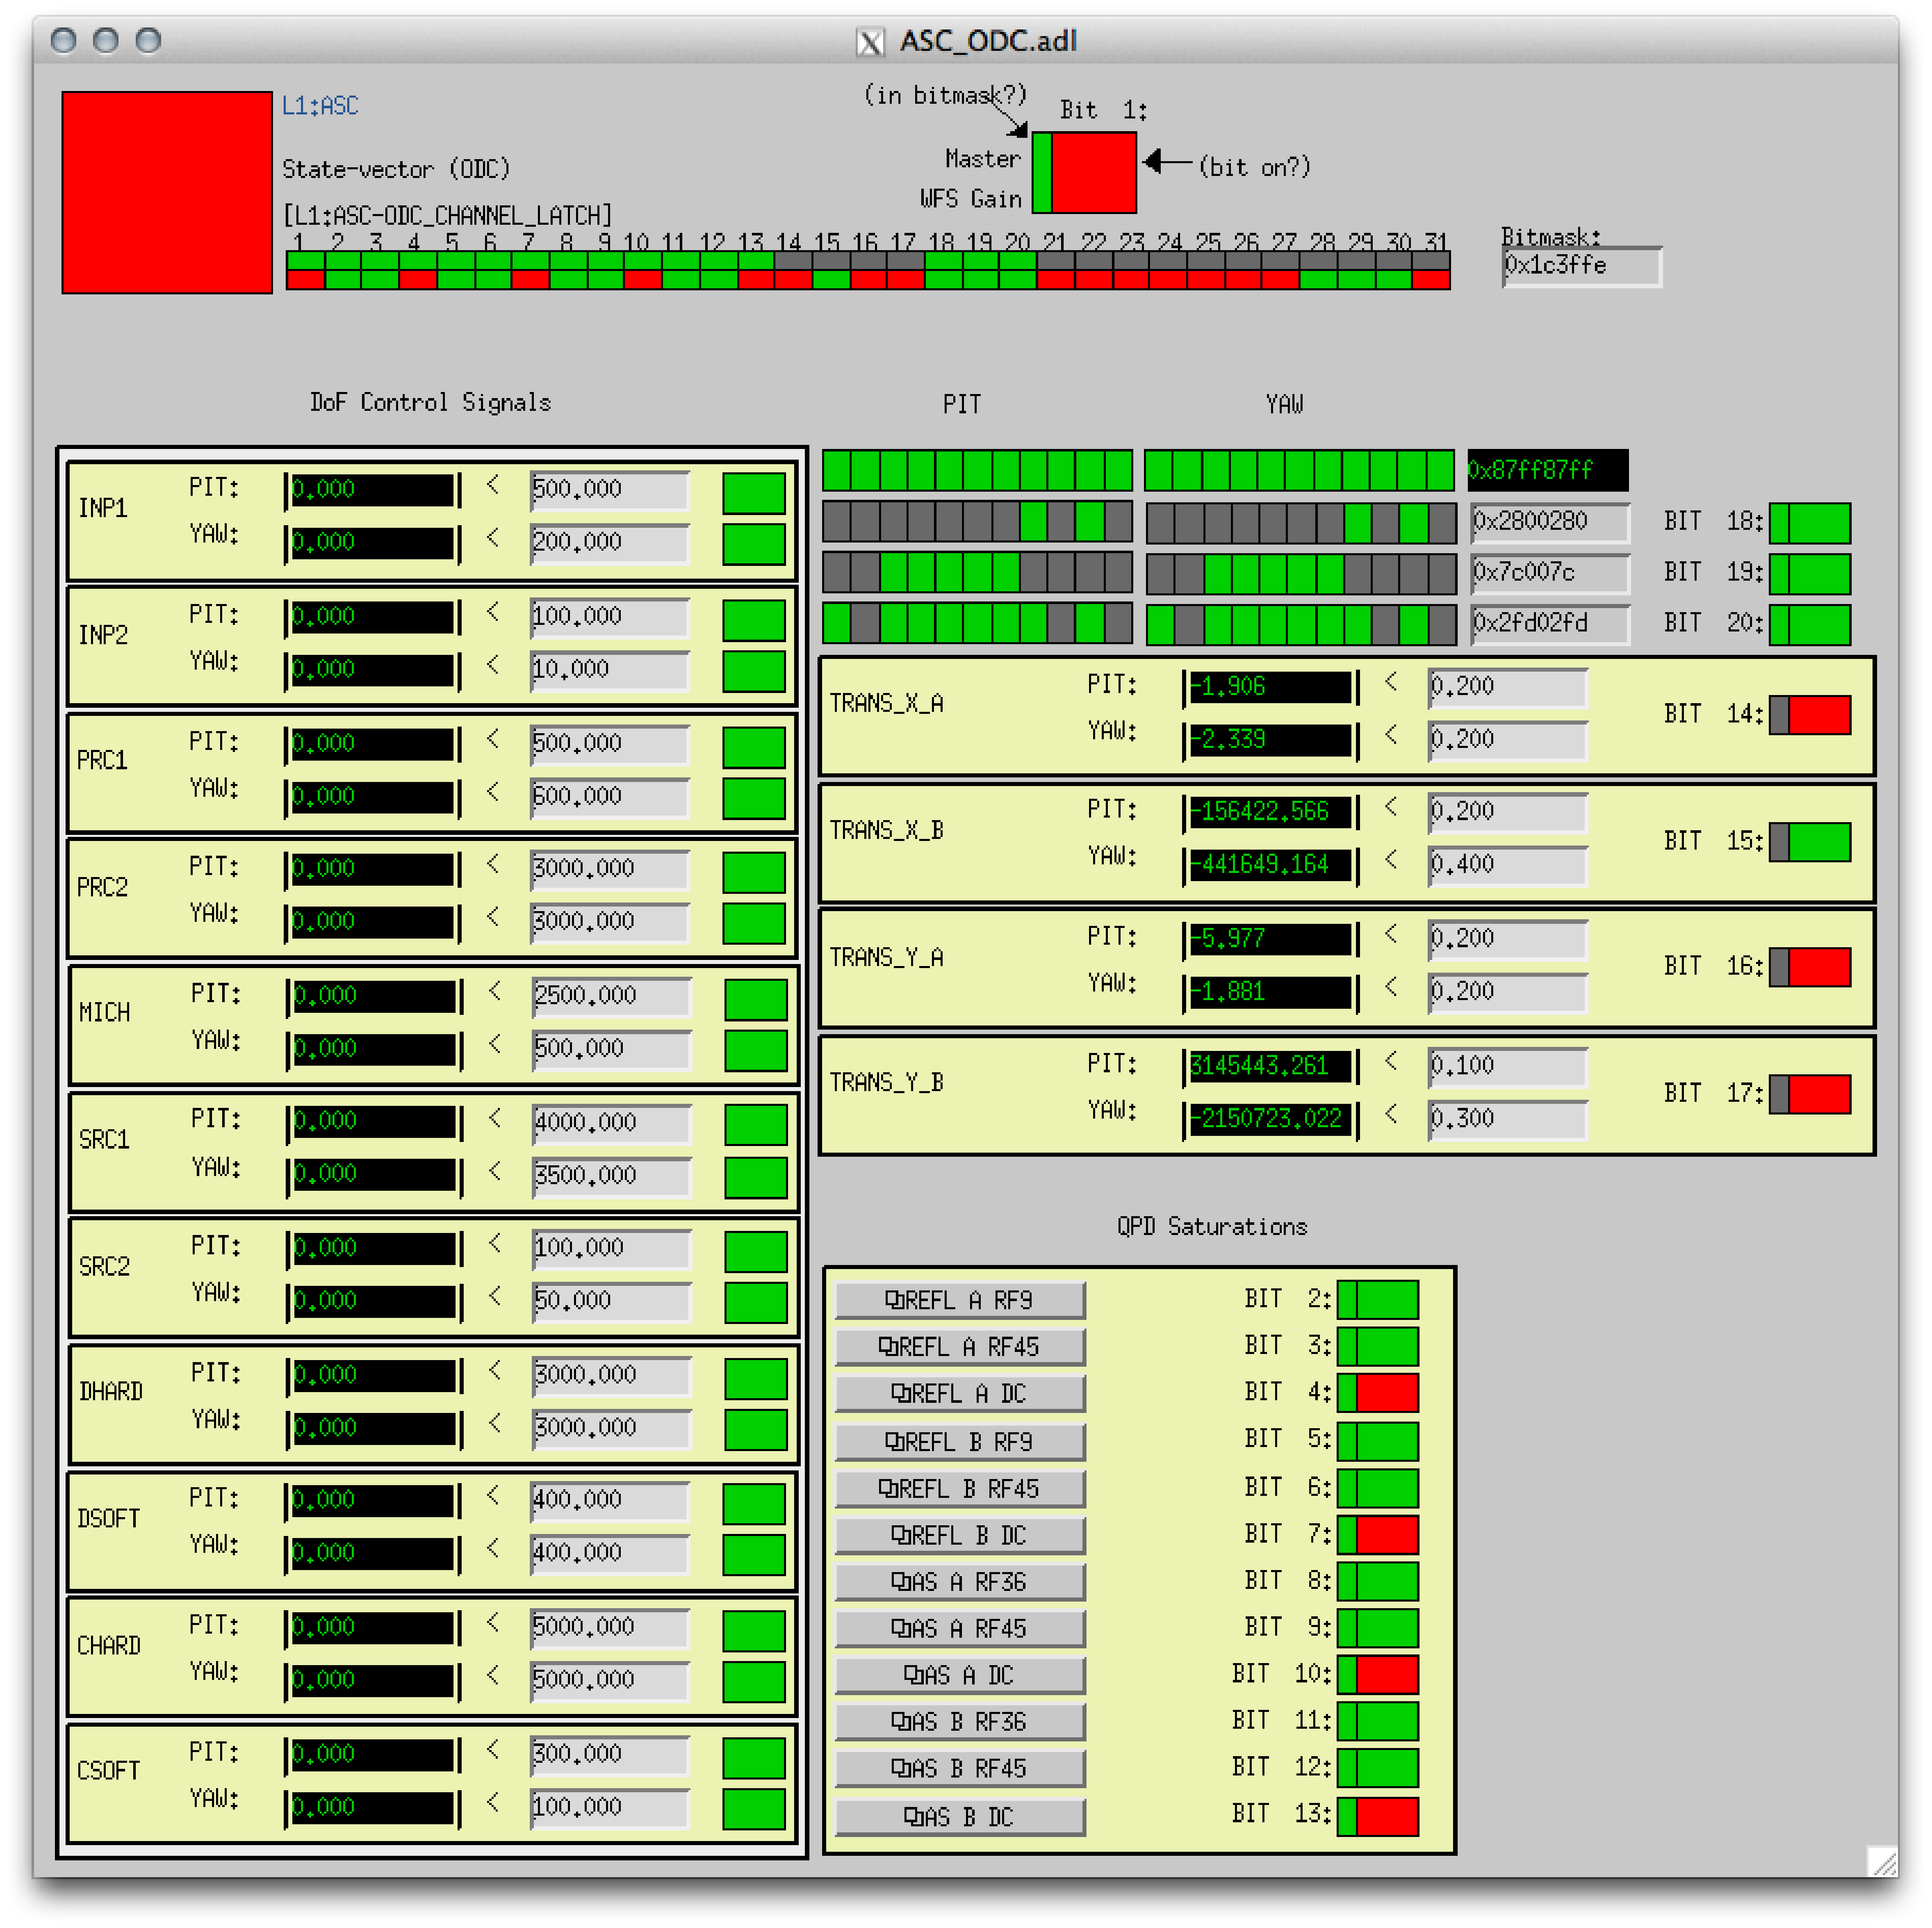
\includegraphics[width=\textwidth]{figures/ODC/ASC_screen}
\caption[ASC ODC Overview Screen]{MEDM screen used to interact with the ASC ODC model. %
         This screen shows the overall state of the ASC subsystem, the state of each %
         alignment degree of freedom in the interferometer, and the state of each %
         quadrant photodiode used to sense misalignments in the interferometer.}
\label{fig:asc-odc}
\end{figure}

Since the ASC subsystem uses quadrant photodiodes, each quadrant must be checked 
for saturation. 
Figure \ref{fig:odc-pd-screen} shows a photodiode monitor screen in the ASC ODC. 
The first and second panels show the readouts of each quadrant of a quadrant 
photodiode in I and Q phase respectively. The absolute value of each signal is 
calculated and compared to a threshold value to see if any quadrants are approaching 
a saturation limit. The third and fourth panels perform checks on the associated 
pitch and yaw readouts from these photodiodes to check for excursions beyond the 
nominal threshold. The nominal values for the pitch and yaw degrees of freedom 
are determined by trending these values over long durations of good interferometer 
performance.

\begin{figure}[ht!]
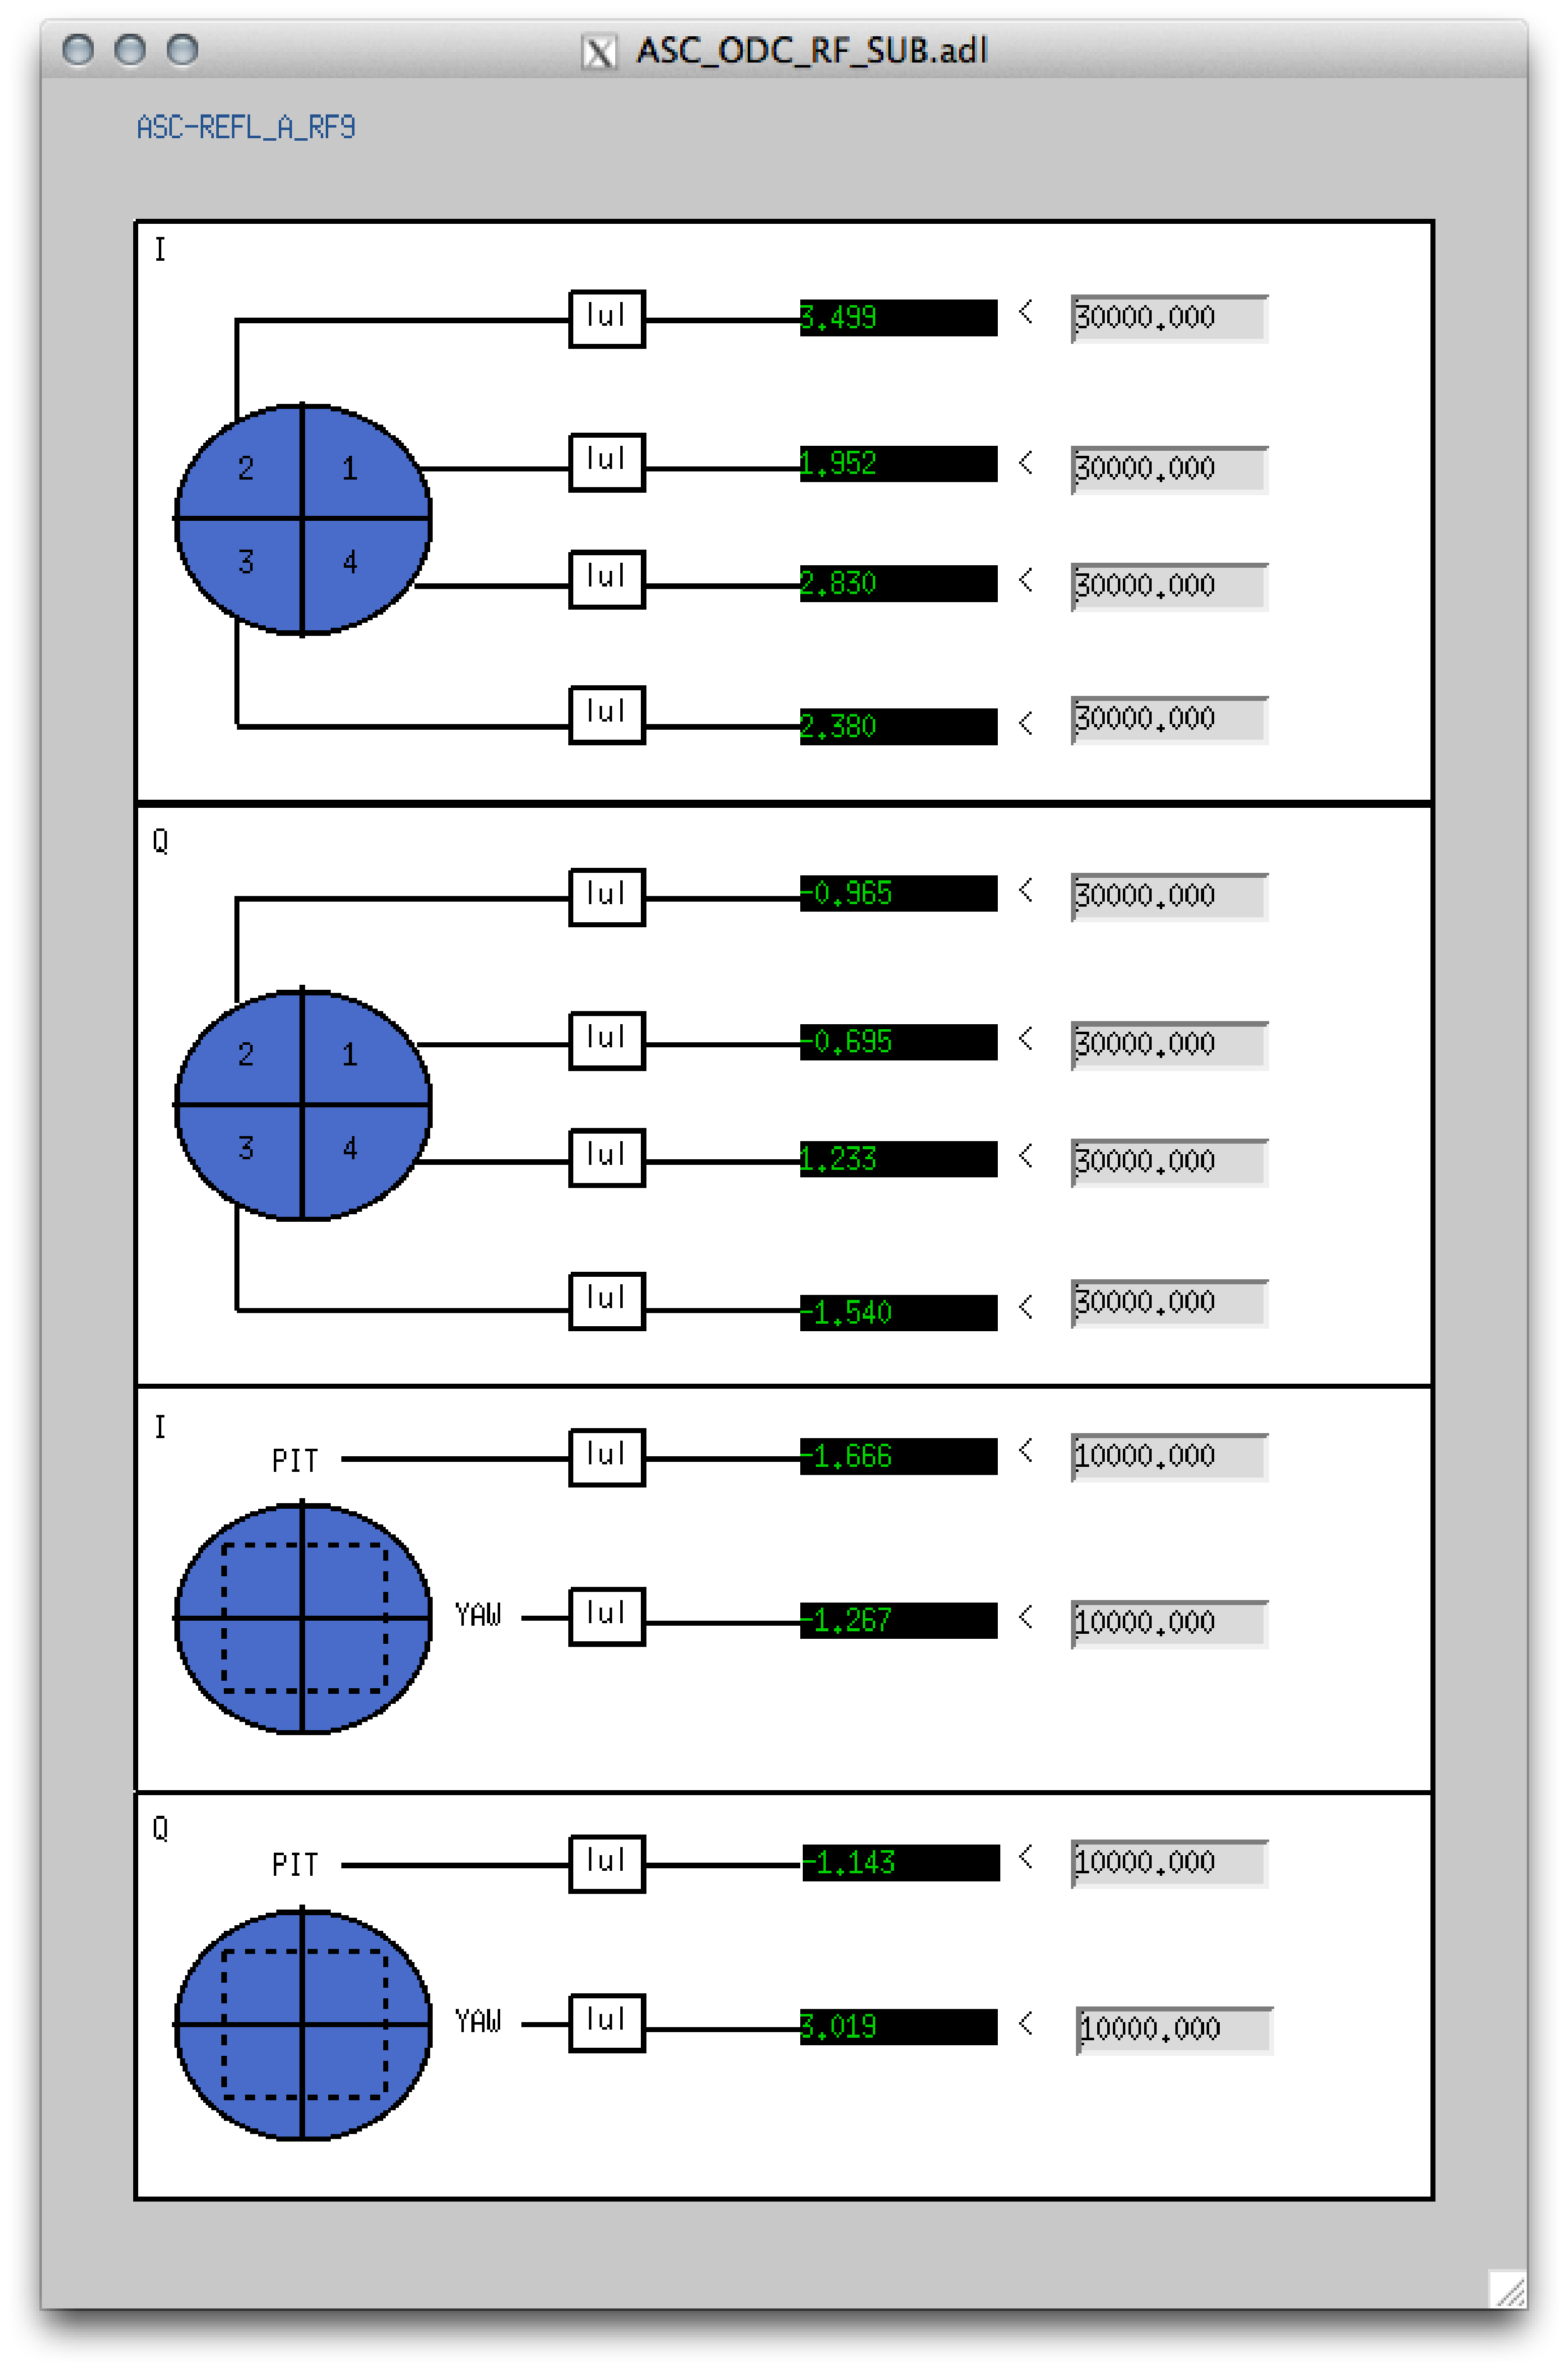
\includegraphics[width=0.7\textwidth]{figures/ODC/PD_screen}
\caption[ASC ODC Photodiode Monitor in MEDM]{ODC monitor for ASC photodiode in MEDM}
\label{fig:odc-pd-screen}
\end{figure}

\subsection{Summary pages}

The ASC subsystem also has an accompanying set of summary pages that keep a running 
record of its state. These summary pages are designed similarly to the LSC summary 
pages, including time-series of the control signals for each alignment degree of freedom, 
saturation monitors for the ASC photodiodes,  
and ODC plots indicating the state of each degree of freedom.

\section{ODC Results}

The ODC system was designed and implemented in the engineering runs that preceded the 
first observing run. During the first observing run, the first efforts were made to 
use the information reported by the ODC models to flag and understand noisy data. 
The most useful 
used the excess noise in the Michelson pitch degree of freedom to flag upstream 
electronics issues that caused loud glitches in $h(t)$. There is also evidence 
that the overall alignment status reported by the ASC ODC can be used as an early 
warning that the interferometer is going to drop out of its nominal operational 
state.

\subsection{MICH ODC as a witness of RF45 glitches}

The ODC channel built to monitor the Michelson (MICH) pitch degree of freedom 
was used to generate vetoes used in O1 analyses. Throughout O1, the H1 
interferometer was prone to a glitch mechanism driven by malfunctions in 
RF electronics used to generate frequency sidebands on the carrer beam. 
These RF sidebands are used to control auxiliary degrees of freedom in the 
interferometer, including the length of the small Michelson interferometer 
formed by the beamsplitter and the two ITMs. When the RF electronics glitched, 
the error signals of these cavities would also glitch, causing excess motion 
in the auxiliary degrees of freedom that was witnessed by ODC monitors set 
up to monitor the control signal of the MICH alignment control loops. 

Figure \ref{fig:mich-odc-example} 
shows the correlation between the witness channel for this ODC channel 
and glitches in $h(t)$ as identified by Omicron. Figure \ref{subfig:mich-odc-timeseries} 
shows a timeseries the control signal of the MICH pitch control loop. The ODC threshold, 
set at a value of 250 for this particular channel, is indicated by the green dotted 
line. Any time the control signal crosses this threshold, a segment is created to 
indicate that the control loop is not in a nominal operating state. Figure 
\ref{subfig:mich-odc-omicron} shows the $h(t)$ Omicron triggers over the same 
duration. When the MICH pitch control point has a high variance, for example 
in the first 1.5 hours of the plot, there is an 
overall increase in the rate of high SNR Omicron triggers, indicating that 
this ODC channel is witnessing alignment fluctuations that couple into the 
output of the interferometer. 

\begin{figure}[ht!]%
\subfloat[]{
  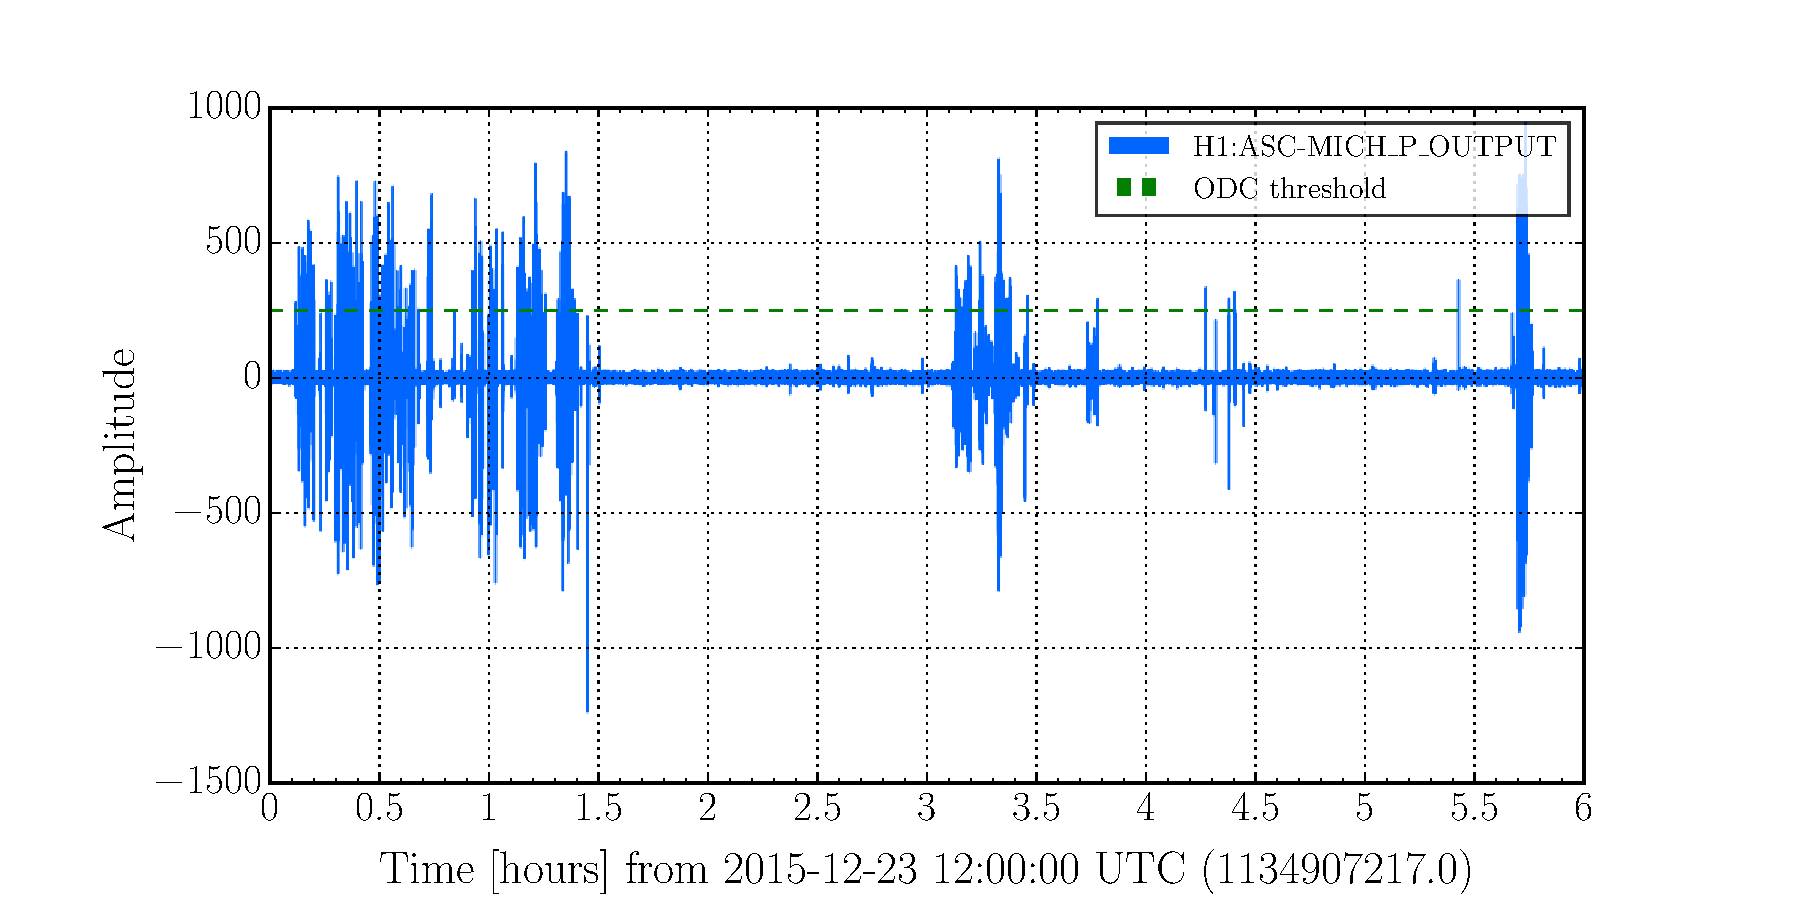
\includegraphics[width=\textwidth]{figures/detchar/MICH_P_OUTPUT_ODC}
  \label{subfig:mich-odc-timeseries}
  }

\subfloat[]{
  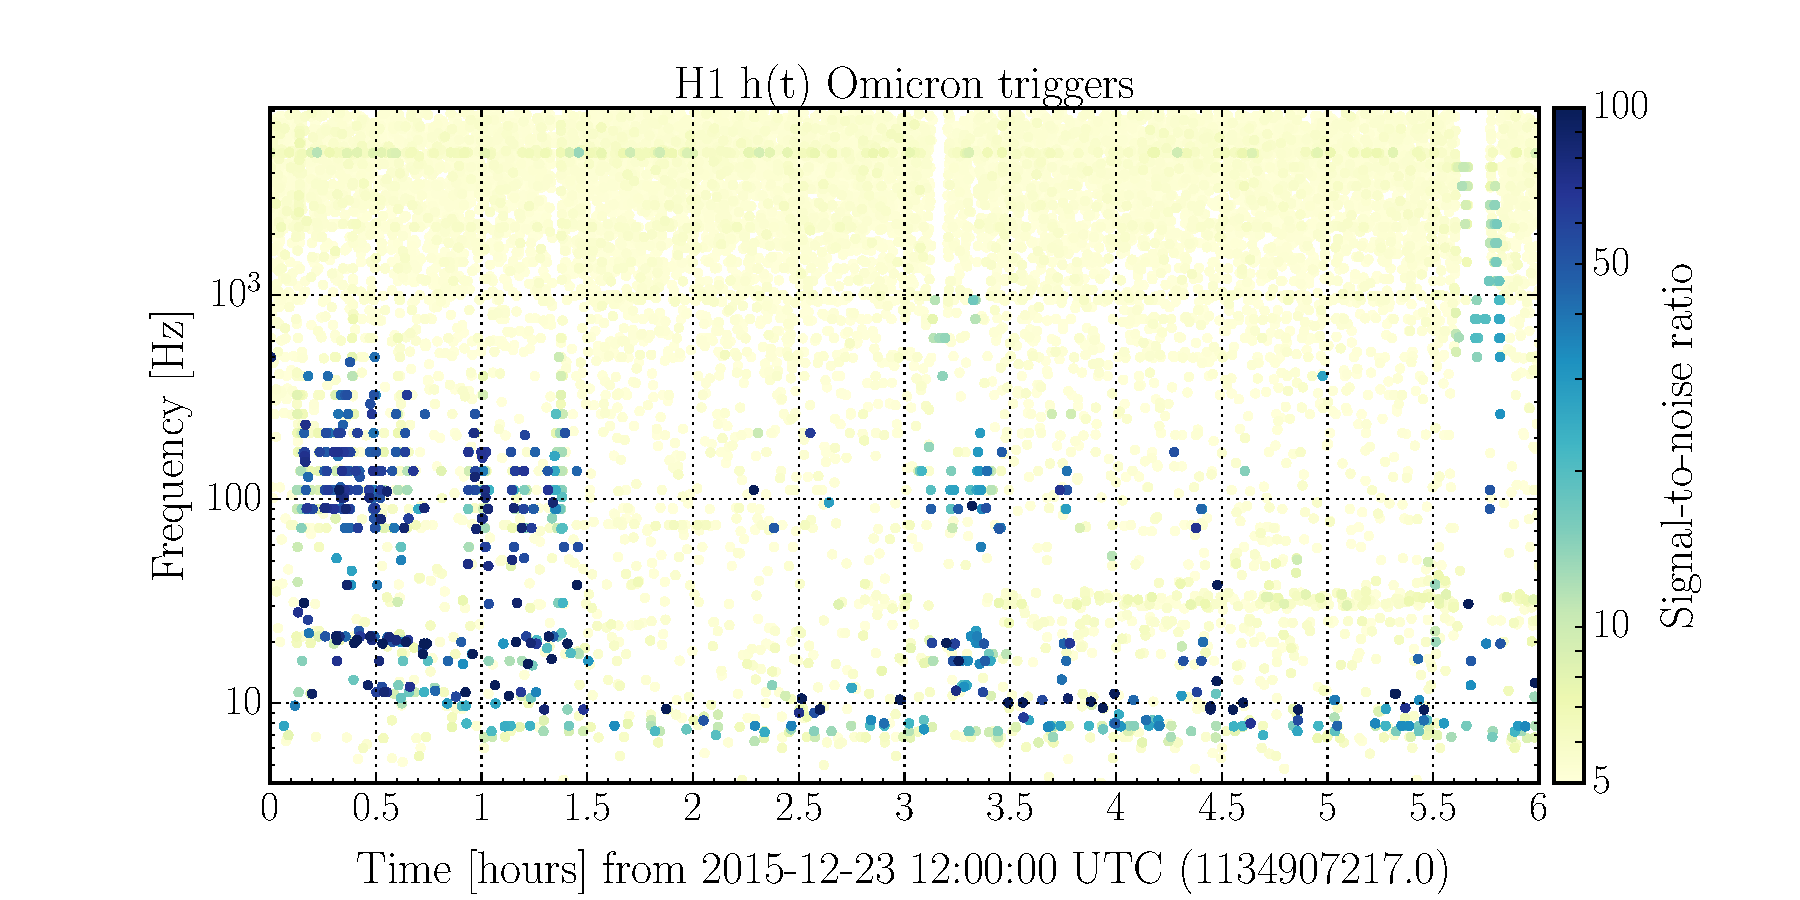
\includegraphics[width=\textwidth]{figures/detchar/Omicron_MICH_ODC}
  \label{subfig:mich-odc-omicron}
  }
\caption[ODC threshold on MICH pitch]{%
         An example of an ODC channel witnessing RF electronics issues, which %
         manifested as angular fluctuations in the vertex degrees of freedom %
         at H1. Figure \ref{subfig:mich-odc-timeseries} shows the ODC threshold %
         marking fluctuations in the MICH pitch degree of freedom. Figure %
         \ref{subfig:mich-odc-omicron} shows the associated Omicron triggers from %
         $h(t)$ at the same time. The storms of loud triggers between 10 - 400 Hz %
         are coincident with times flagged by this ODC monitor.}
\end{figure}\label{fig:mich-odc-example}

This coupling can be quantified using the veto evaluation tool (VET). The 
segments generated by this ODC channel are very efficient at vetoing high SNR 
Omicron triggers. VET reports that these segments veto Omicron triggers with SNR 
$>$ 8 with an efficiency:deadtime ratio of 47.16, indicating that these segments 
veto a large number of high SNR Omicron triggers with very little deadtime. These 
veto segments were included in the veto definer files that were distributed to 
the CBC and Burst searches in O1. 



\Chapter{Data Quality Vetoes}
\label{ch:Vetoes}
As discussed in Chapters \ref{ch:CBCSearches} and \ref{ch:instrumentalDetchar}, the data at the 
output of the LIGO interferometers contain non-Gaussian, transient noise artifacts. 
Chapter \ref{ch:instrumentalDetchar}, \ref{ch:IMCUpconversion}, and \ref{ch:ODC} detail the efforts 
that have been made to understand and remove transient noise in the LIGO interferometers. 
When it was possible, transient noise sources were repaired at the source and the noise was not 
able to impact the output of astrophysical searches. Unfortunately, this is not always possible. 
If a source of transient noise can't be repaired, the noisy data will be processed by astrophysical
search pipelines. 

Transient noise artifacts are 
known to cause loud events at the output of astrophysical searches for gravitational waves, which 
manfiest as a tail in the re-weighted SNR distribution as seen in Figure \ref{subfig:l1-newsnr-hist}. 
The data that comprise this tail of loudest events are the primary target of data quality 
investigations, such as those discussed in Chapter \ref{ch:instrumentalDetchar}. 
If the noise sources can be linked to a 
systematic instrumental cause or a period of highly irregular instrumental performance, 
they can be flagged and removed from the analysis in the form of a 
data quality veto.

It is important to note that data quality vetoes are produced for all analysis time based
on systematic instrumental conditions without any regard for the presence of gravitational wave
signals. All data are treated equally; the removal of data with excess noise has the ability to
remove real gravitational wave signals as well as background events.
There are two types of vetoes implemented in the PyCBC search: category 1 and
category 2.

\section{Veto categories}

Category 1 (CAT1) vetoes are intended to mark times when significant instrumental issues are present
and the data should not be used in any analysis. CAT1 flags often indicate time
when the character of the data has drastically changed and should not be combined
with noise estimations from times of nominal performance.
An example of this from O1 is an electronics failure that dramatically changes the character of the
background noise and creates noise transients at a very high rate.
As such, CAT1 vetoes remove time at the input to the PyCBC search pipeline. This ensures that
severely problematic data are not used for background noise estimations and that no triggers will be
generated at these times.

Category 2 (CAT2) vetoes are intended to mark short, noisy times that
that should not be treated as clean data. CAT2 flags are often
used to flag transients that could potentially generate loud triggers, but do not
corrupt the surrounding data badly enough that they need to be excluded at the input to the pipeline.
An example of this is from O1 is a transient electronics saturation that only impacts the output
data for 1 second.  Times designated
as CAT2 will still be used to compute background noise estimations for the matched filter search,
but any triggers generated
during those times will be excluded before background trigger distributions are calculated.

Further details on the application of CAT1 and CAT2 vetoes in the first observing run
are available in a paper detailing the transient noise in the interferometers at the
time of GW150914 \cite{GW150914-DETCHAR}.

\section{Quantifying the effects of data quality vetoes}
Does removing noisy data with data quality vetoes improve the output of the PyCBC search pipeline?

To test the effects of data quality vetoes, the PyCBC search pipeline was run multiple times with
varying levels of noisy data removed. The first analysis, labeled
``All vetoes applied'', used the full range of relevant data quality vetoes. The second
analysis, labeled ``No CAT2 applied'', omitted category 2 data quality vetoes. The third and final
analysis, labeled ``No CAT1 or CAT2 applied'', omitted all data quality vetoes.
Gating is internal to the search pipeline and was applied in all of the analyses.

The bank of CBC waveform templates used in the PyCBC search is divided into three bins
\cite{GW150914-CBC}. The significance of any candidate gravitational wave found in
coincidence between the two interferometers is calculated relative to the background in its bin.
Waveforms with different parameters will respond to instrumental transients in different ways.
This binning is performed so that any foreground triggers are compared to a background
generated from similar waveforms.
As such, the effects of removing data from the PyCBC search are variable depending on
which bin is considered. It should be noted that the actual gravitational wave signals
discovered in the PyCBC search,
GW150914 and GW151226, were part of a full search that was broken into 3 bins but reported
as a single table of results. Because of this,
their reported false alarm rates include a trials factor of 3. The comparisons made in Sections
\ref{sec:GW150914analysis} and \ref{sec:GW151226analysis} are done on a bin-by-bin basis,
so the quoted rates have not been divided by 3. This is an overall factor of 3 change
that does not affect the relative change in significance between the various analysis
configurations.

The first bin is called the binary neutron star (BNS) bin and contains all waveforms
with an $M_{chirp} < 1.74$.
The second bin is the edge bin, which is defined based on the peak frequency ($f_{peak}$)
of each CBC waveform.
These are waveforms that are typically rather short in duration and are comprised of
both binary black hole (BBH) and neutron star-black hole (NSBH) binary waveforms
with high masses and anti-aligned effective spins.
In the analysis containing GW150914, the edge bin was
defined by $f_{peak} <$ 220 Hz. In the analysis containing GW151226, the edge been
was defined by $f_{peak} <$ 100 Hz.
The third bin is the bulk bin, which contains all remaining
waveforms needed to span the parameter space of the search. This contains BBH and NSBH
waveforms with a variety of mass ratios and spins.

To study how the removal of noisy data affects the background distributions, we consider a
hypothetical detection candidate at $\hat{\rho}_{c} = 11.3$, which corresponds to
$\hat{\rho} = 8$ in each detector. Figure \ref{fig:gaussian-rate} compares the distribution
of re-weighted SNR in Gaussian noise to that of real detector data.
In Gaussian noise, the re-weighted SNR distribution is limited to
$\hat{\rho} <$ 8 for single
detector triggers. A single detector trigger with $\hat{\rho} =$ 8 would stand out against this
background distribution as the loudest event in each detector. However, this is well within
the region of the re-weighted SNR distribution that is commonly obscured by instrumental transients
and non-Gaussian features in the data. Figure \ref{fig:gaussian-rate} shows significant tails
of loud triggers in each detector beyond $\hat{\rho} = 8$. It is this region, where the
re-weighted SNR histograms contain non-Gaussian features, that data quality
studies aim to improve.
The hypothetical detection candidate at $\hat{\rho} = 8$ is a very useful threshold case:
loud enough to be interesting, but quiet
enough that its significance should be impacted by instrumental transients and data quality
vetoes.

\begin{figure}[ht!]%
\centering
  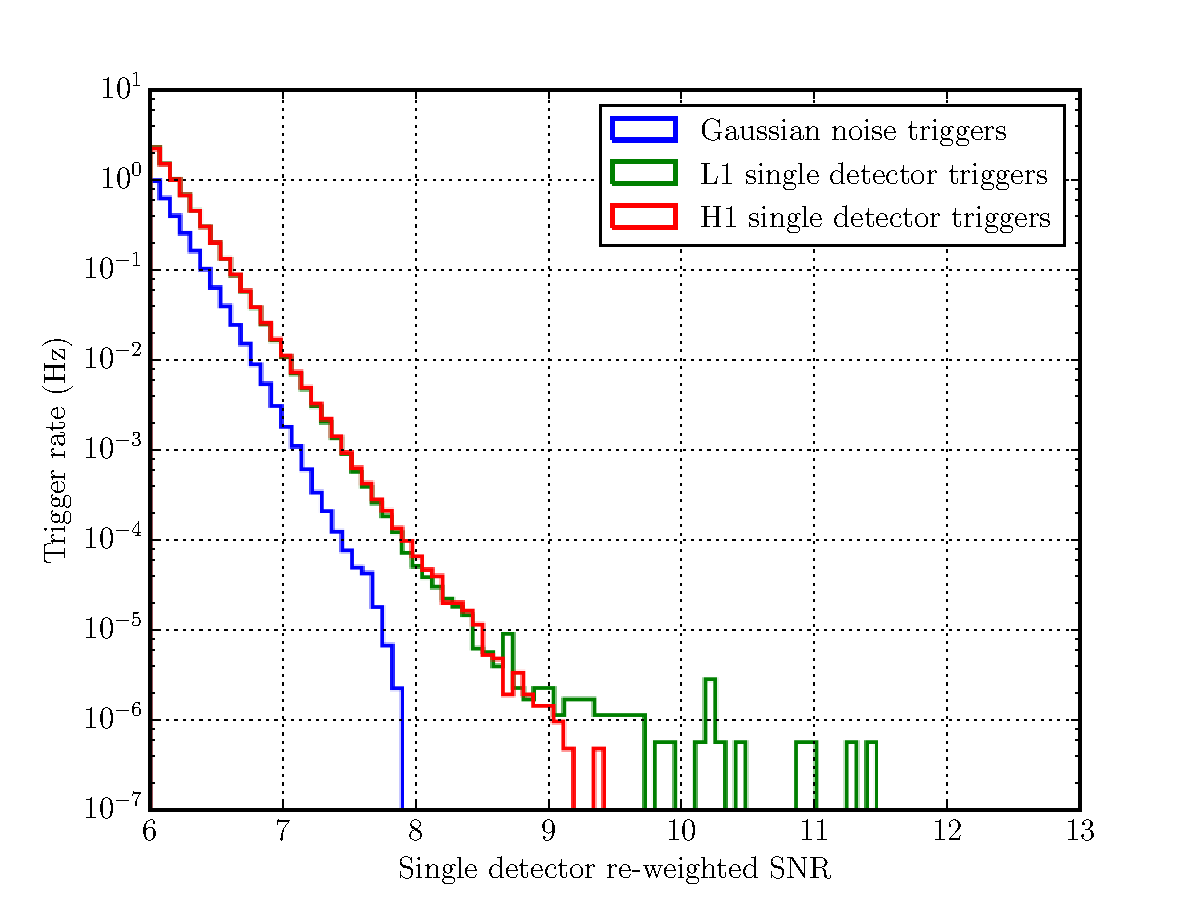
\includegraphics[width=0.8\textwidth]{figures/o1-cbc-dq-paper/H1-L1-Gaussian-newSNR-rate-hist}
  \caption[Rate histogram of PyCBC triggers vs. Gaussian noise]{A rate histogram %
           comparing the re-weighted SNR distribution in Gaussian %
           noise to that of real detector data. In Gaussian noise, the re-weighted %
           SNR distribution falls off before reaching $\hat{\rho} = 8$. %
           The distributions from real detector noise show extensive tails beyond %
           $\hat{\rho} = 8$ in addition to having an overall higher trigger rate.}
\label{fig:gaussian-rate}
\end{figure}





\Chapter{Effects of Data Quality Vetoes on the Analysis Containing GW150914}
\label{ch:GW150914-DQ}
Effects of DQ on analysis containing GW150914

\section{BNS bin}

\section{Bulk bin}

\subsection{LVT151012}

\section{Edge bin}

\subsection{GW150914}




\Chapter{Effects of Data Quality Vetoes on the Analysis Containing GW151226}
\label{ch:GW151226-DQ}
The extended analysis containing GW151226 lasted from December 3, 2015 - January 19, 2016 and
contained a total of 16.7 days of coincident detector data.
After category 1 vetoes were removed, 16 days of coincident data remained. After
category 2 vetoes were removed, 15.8 days of coincident remained and were used in the
final analysis.
This analysis time provided
an extended background estimation for the binary black hole merger GW151226 \cite{GW151226},
which was detected by the aLIGO interferometers on December 26, 2015.

\section{BNS bin}

The BNS bin shows a slight improvement when data quality vetoes are included.
Figure \ref{fig:bns-bin-far-GW151226} shows the background distributions in the BNS
bin before and after removing data with vetoes. The most significant
effect is that the loudest event in the background is at a higher re-weighted SNR;
the loudest background event is at $\hat{\rho}_{c} =$ 10.96 rather
than $\hat{\rho}_{c} =$ 10.6.

\begin{figure}[!ht]%
\centering
  \subfloat[]{
  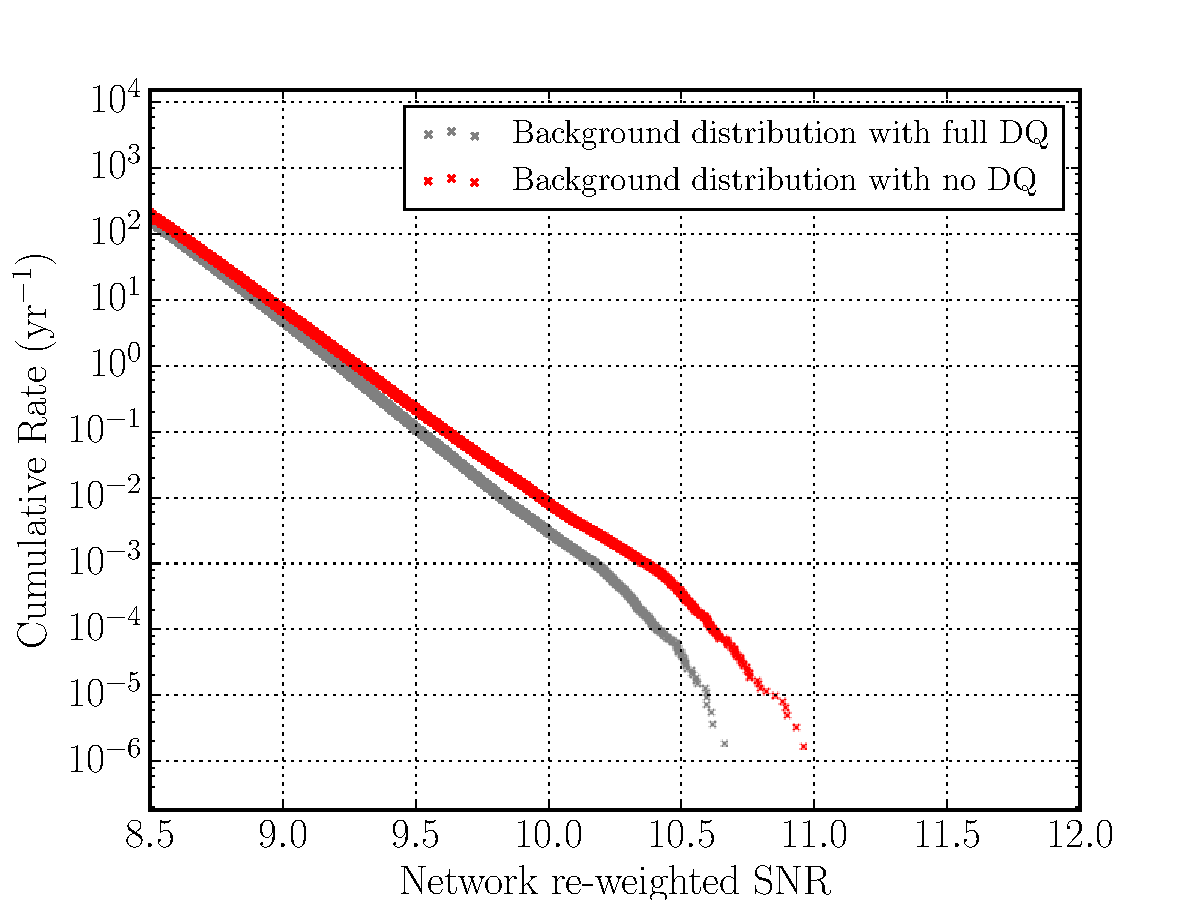
\includegraphics[width=0.495\textwidth]{figures/o1-cbc-dq-paper/bns_bin_GW151226_DQ_comparison}
  \label{subfig:bns-bin-gw151226-rate}
  }
  \subfloat[]{
  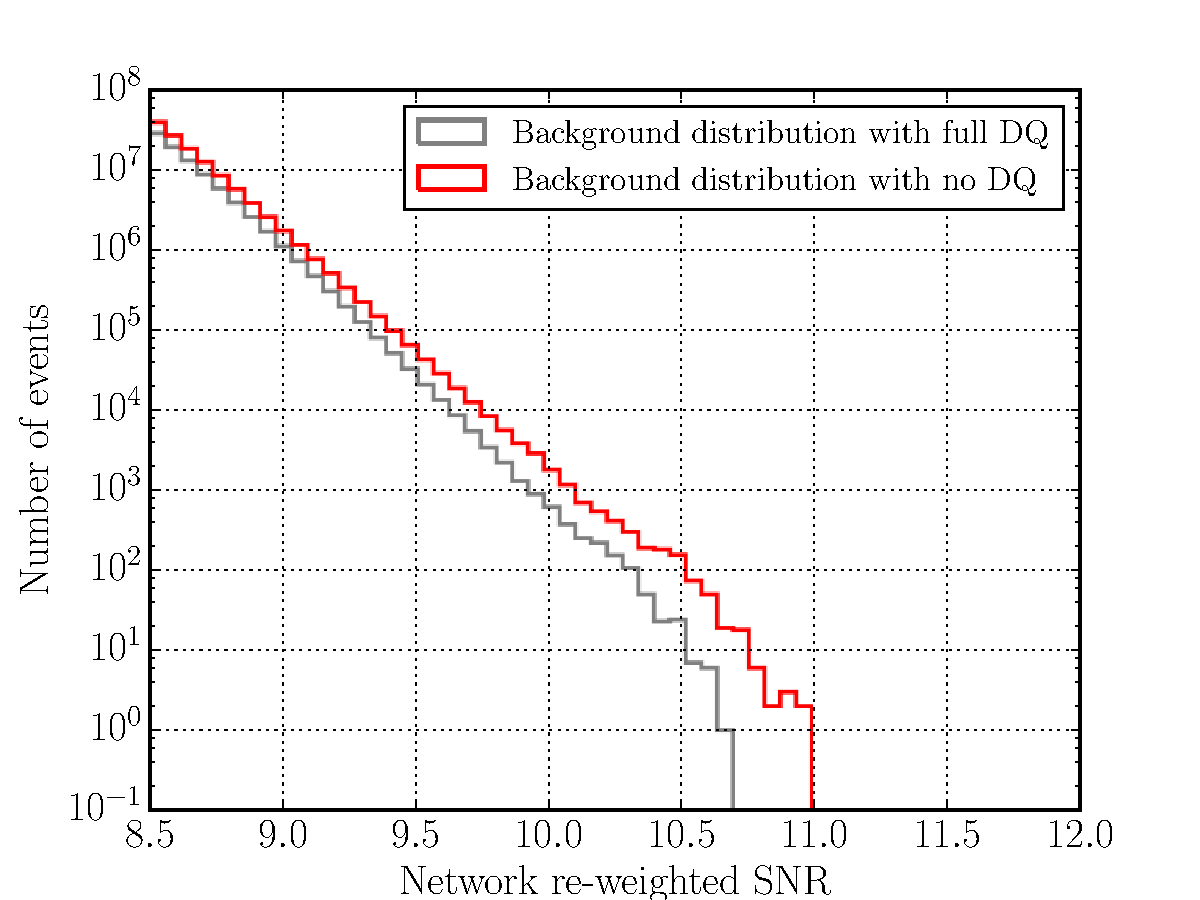
\includegraphics[width=0.495\textwidth]{figures/o1-cbc-dq-paper/bns_bin_GW151226_DQ_raw_hist}
  \label{subfig:bns-bin-gw151226-raw}
  }
  \caption[BNS bin histograms - GW151226 analysis]{The background distribution in the BNS bin before and after applying data quality (DQ) vetoes. %
           (\ref{subfig:bns-bin-gw151226-rate}) The cumulative rate of background triggers %
           in the BNS bin as a function of re-weighted SNR. %
           (\ref{subfig:bns-bin-gw151226-raw}) A histogram of background triggers %
           in the BNS bin. % 
           The red traces indicate the %
           distribution of background triggers without noisy data removed % 
           and the gray traces indicate the distribution %
           of background triggers with all data quality vetoes applied. %
           The BNS bin shows minimal improvement. %
           With noisy data removed, the loudest background event is at $\hat{\rho}_{c} =$ 10.6. %
           Without removing any data, the loudest background event is at $\hat{\rho}_{c} =$ 10.96. % 
          }
\label{fig:bns-bin-far-GW151226}
\end{figure}

Although the removal of problematic data has a visible impact on the background of the BNS bin,
the resulting distribution is still not limiting to the search. In both cases, the
hypothetical detection candidate at $\hat{\rho}_{c} =$ 11.3 would be the loudest event in the analysis.
The difference in false alarm rate is quantified in Table \ref{table:151226-bns-far}.

\begin{table}[!ht]%
  \begin{center}
    \begin{tabular}{lcc}
      \hline
      Analysis configuration & False alarm rate ($yr^{-1}$) & False alarm probability \\ \hline
      All vetoes applied & $1.82\times10^{-6}$  & $7.60\times10^{-8}$ \\
      No CAT2 applied & $1.77\times10^{-6}$ & $7.48\times10^{-8}$ \\
      No CAT1 or CAT2 applied & $1.63\times10^{-6}$ & $7.18\times10^{-8}$ \\ \hline
    \end{tabular}
  \end{center}
  \caption[BNS bin FAR - GW151226 analysis]{Table of false alarm rates and probabilities at $\hat{\rho}_{c} =$ 11.3 for several analysis configurations. %
           The difference in false alarm rate between the different configurations is negligible %
           in the BNS bin.}
  \label{table:151226-bns-far}
\end{table}

\section{Bulk bin}

The bulk bin benefited from the application of data quality vetoes. Figure
\ref{fig:bulk-bin-far-GW151226} shows the bulk bin background distribution before and after
data quality vetoes applied. The first notable
effect is that the loudest background event is at $\hat{\rho}_{c} =$ 14.8 rather than
$\hat{\rho}_{c} =$ 11.8. This effect
limits the values of $\hat{\rho}_{c}$ for which a significant detection could be claimed.
The second effect is the visible separation between the two curves, indicating an
increase in false alarm rate for any trigger with $\hat{\rho}_{c} >$ 9. An example of this is
quantified by once again considering a hypothetical detection candidate at $\hat{\rho}_{c} =$ 11.3.
At this value of $\hat{\rho}_{c}$, there is a factor of 800 reduction in false alarm rate when
data quality vetoes are applied, as detailed in Table \ref{table:GW151226-bulk-far}.
The application of CAT2 vetoes has a positive impact on this bin, providing a factor of 54
reduction in false alarm rate compared to an analysis where only CAT1 vetoes are applied.

\begin{figure}[!ht]%
\centering
  \subfloat[]{
  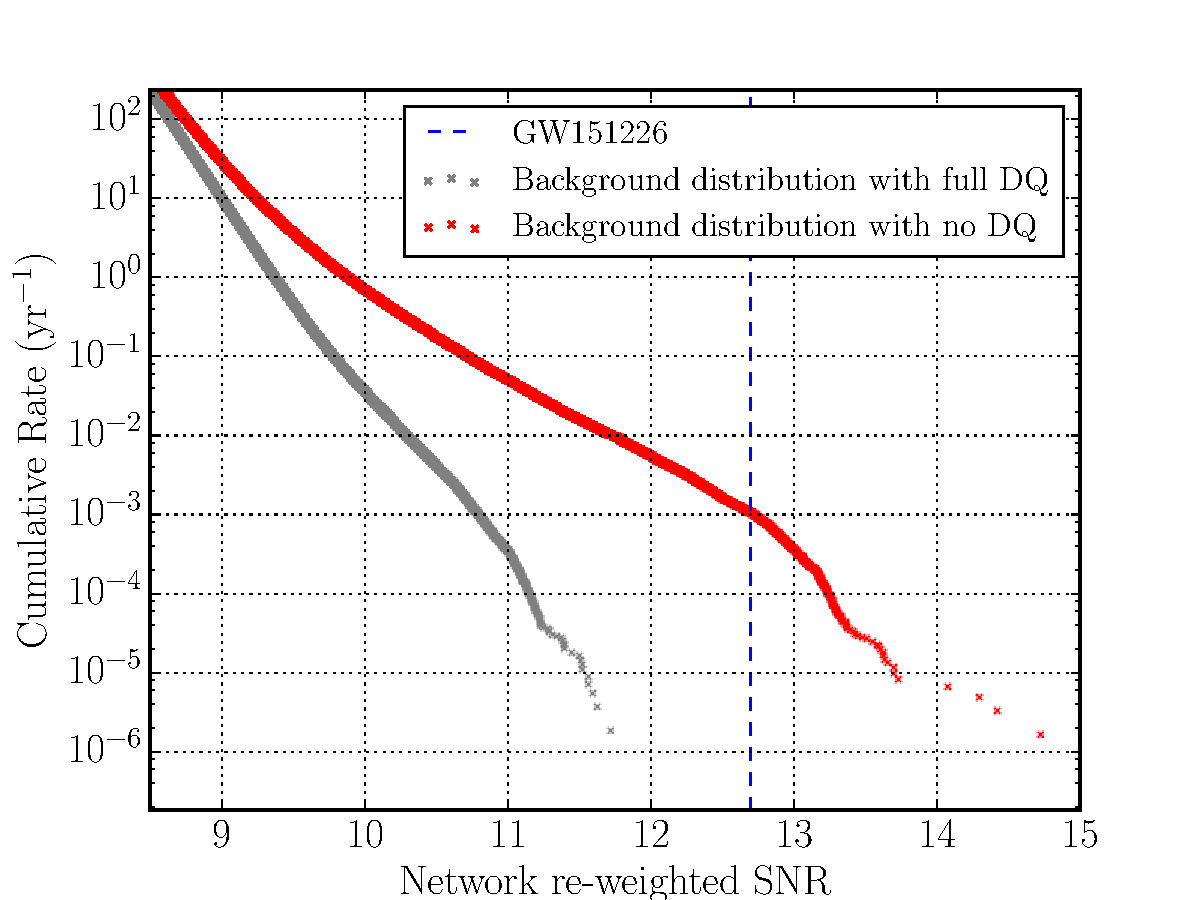
\includegraphics[width=0.495\textwidth]{figures/o1-cbc-dq-paper/bulk_bin_GW151226_DQ_comparison}
  \label{subfig:bulk-bin-gw151226-rate}
  }
  \subfloat[]{
  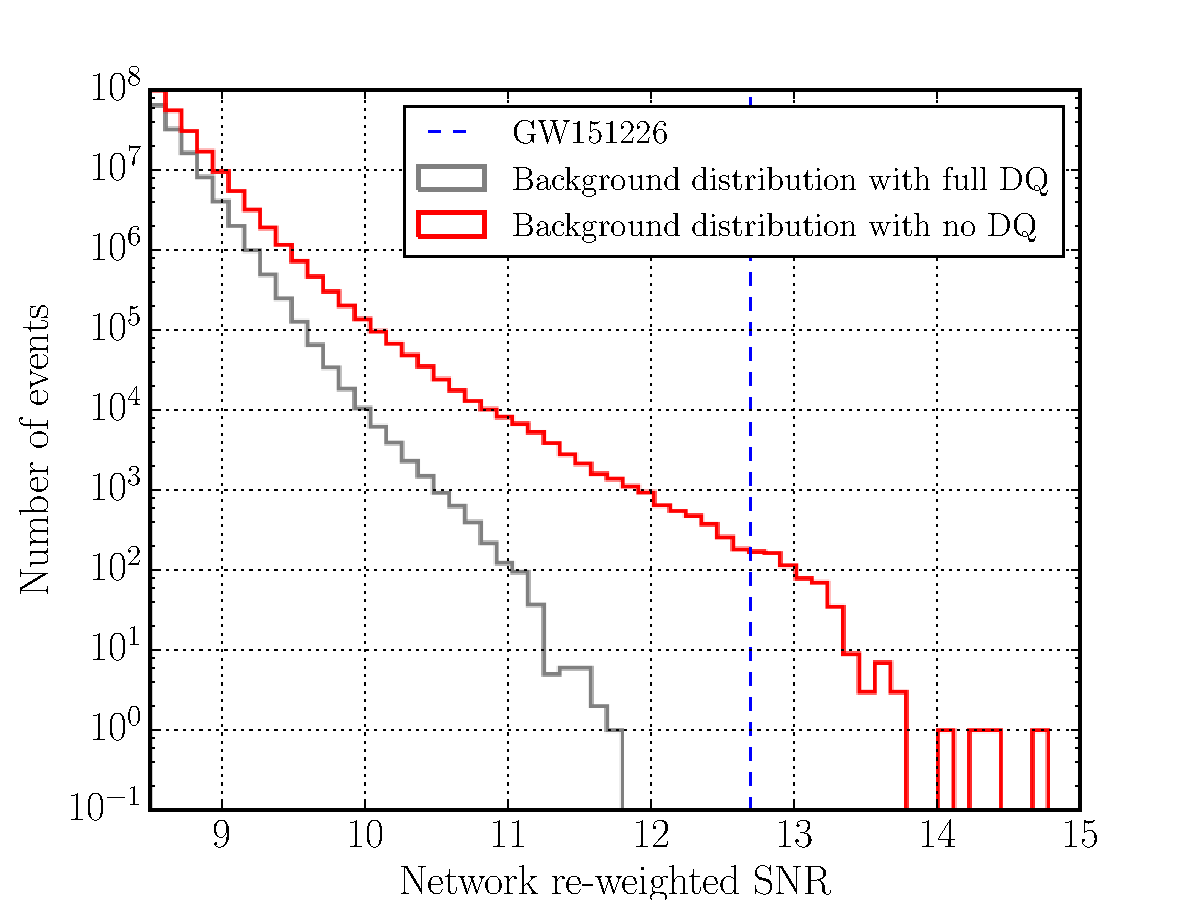
\includegraphics[width=0.495\textwidth]{figures/o1-cbc-dq-paper/bulk_bin_GW151226_DQ_raw_hist}
  \label{subfig:bulk-bin-gw151226-raw}
  }
  \caption[Bulk bin histograms - GW150914 analysis]{The background distribution in the bulk bin before and after applying data quality %
           (DQ) vetoes. % 
           (\ref{subfig:bulk-bin-gw151226-rate}) The cumulative rate of background triggers %
           in the bulk bin as a function of re-weighted SNR. %
           (\ref{subfig:bulk-bin-gw151226-raw}) A histogram of background triggers %
           in the bulk bin. % 
           The red traces indicate the %
           distribution of background triggers without noisy data removed, %
           the gray traces indicate the distribution %
           of background triggers with all data quality vetoes applied. %
           The dotted line indicates GW151226, which was recovered with $\hat{\rho}_{c} =$ 12.7. %
           If no data quality vetoes are applied, the tail of loud background triggers extends to %
           $\hat{\rho}_{c} =$ 14.8 instead of $\hat{\rho}_{c} =$ 11.8. % 
           The impact of this change is apparent when considering GW151226, which is no %
           longer the loudest event in this bin (see Section \ref{sec:GW151226}). %
          }
\label{fig:bulk-bin-far-GW151226}
\end{figure}

\begin{table}[!ht]%
  \begin{center}
    \begin{tabular}{lcc}
      \hline
      Analysis configuration & False alarm rate ($yr^{-1}$) & False alarm probability \\ \hline
      All vetoes applied & $3.10\times10^{-5}$  & $1.29\times10^{-6}$ \\
      No CAT2 applied & $1.70\times10^{-3}$ & $7.23\times10^{-5}$ \\
      No CAT1 or CAT2 applied & $2.48\times10^{-2}$ & $1.10\times10^{-3}$ \\ \hline
    \end{tabular}
  \end{center}
  \caption[Bulk bin FAR - GW151226 analysis]{Table of bulk bin false alarm rates and probabilities at $\hat{\rho}_{c} =$ 11.3 %
           for several analysis configurations. At $\hat{\rho}_{c} =$ 11.3, the false alarm %
           rate decreases by a factor of 800 when data with excess noise is removed from %
           the analysis. Category 2 vetoes are more effective in this bin, providing a factor % 
           of 54 reduction in false alarm rate.}
  \label{table:GW151226-bulk-far}
\end{table}

\subsection{GW151226}\label{sec:GW151226}

The binary black hole system GW151226 was recovered by the PyCBC pipeline
in the bulk bin with $\hat{\rho}_{c} =$ 12.7 \cite{GW151226}.
The significance of GW151226 was improved by the application of data quality
vetoes. These changes in significance are quantified in Table \ref{table:GW151226-far}.
When all data quality vetoes were applied to the analysis, GW151226 was the loudest
event in the bulk bin and has a false alarm rate of 1 per 183000 years.
If noisy data are not removed from the analysis, GW151226 is no longer the loudest
event in the bulk bin and its false alarm rate increases by a factor of 567
to 1 in 320 years. This
increase takes a clear detection ($>$5$\sigma$) and reduces its significance to
that of a more marginal detection candidate (3.9$\sigma$).

\begin{table}[!ht]%
  \begin{center}
    \begin{tabular}{lcc}
      \hline
      Analysis configuration & False alarm rate ($yr^{-1}$) & False alarm probability \\ \hline
      All vetoes applied & $5.46\times10^{-6}$  & $2.28\times10^{-7}$ \\
      No CAT2 applied & $1.06\times10^{-5}$ & $4.49\times10^{-7}$ \\
      No CAT1 or CAT2 applied & $3.1\times10^{-3}$ & $1.38\times10^{-4}$ \\ \hline
    \end{tabular}
  \end{center}
  \caption[GW151226 FAR]{Table of false alarm rates and probabilities of GW151226 for several analysis %
           configurations. The false alarm rate of GW151226 increases by a factor %
           of 567, from 1 in 183000 years to 1 in 320 years, if data with excess noise %
           is not removed from the analysis.}
  \label{table:GW151226-far}
\end{table}

\section{Edge bin}

The background distribution in the edge bin looks dramatically different if data quality
vetoes are not applied. This is not surprising, given that this tuning of the edge bin
is restricted to contain the shortest waveforms with $f_{peak} <$ 100 Hz, which
will have a very short template duration and be susceptible to instrumental transients.
Figure \ref{fig:edge-bin-far-GW151226} shows the background distribution in the edge bin
before and after data quality vetoes have been applied.
The loudest event in this bin with all vetoes applied was at $\hat{\rho}_{c} =$ 15,
which was already inconveniently loud for a search hoping to recover a signal in this
bin. When noisy data are not removed from the analysis, the loudest background event is at
$\hat{\rho}_{c} =$ 18.3, which further restricts the region where a confident
detection could be made.

\begin{figure}[!ht]%
\centering
  \subfloat[]{
  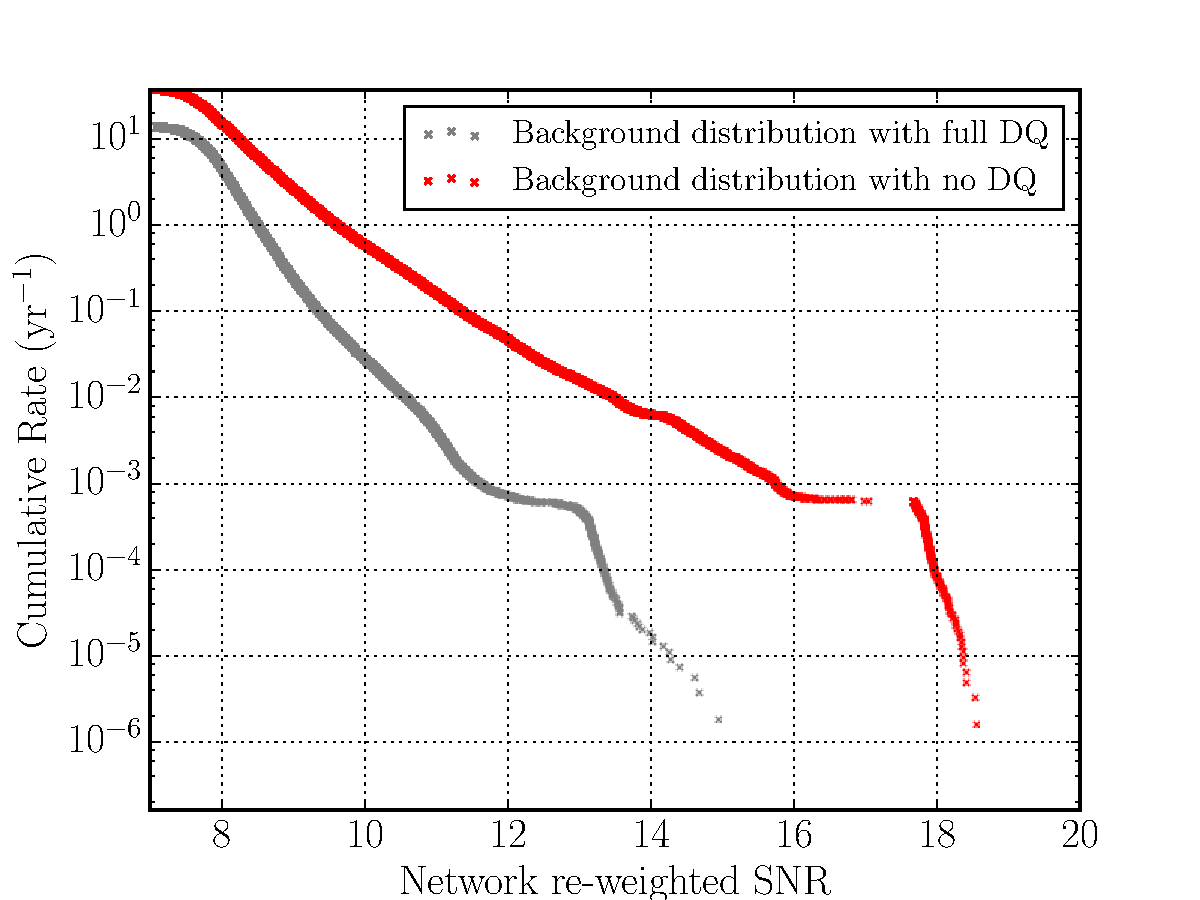
\includegraphics[width=0.495\textwidth]{figures/o1-cbc-dq-paper/edge_bin_GW151226_DQ_comparison}
  \label{subfig:edge-bin-gw151226-rate}
  }
  \subfloat[]{
  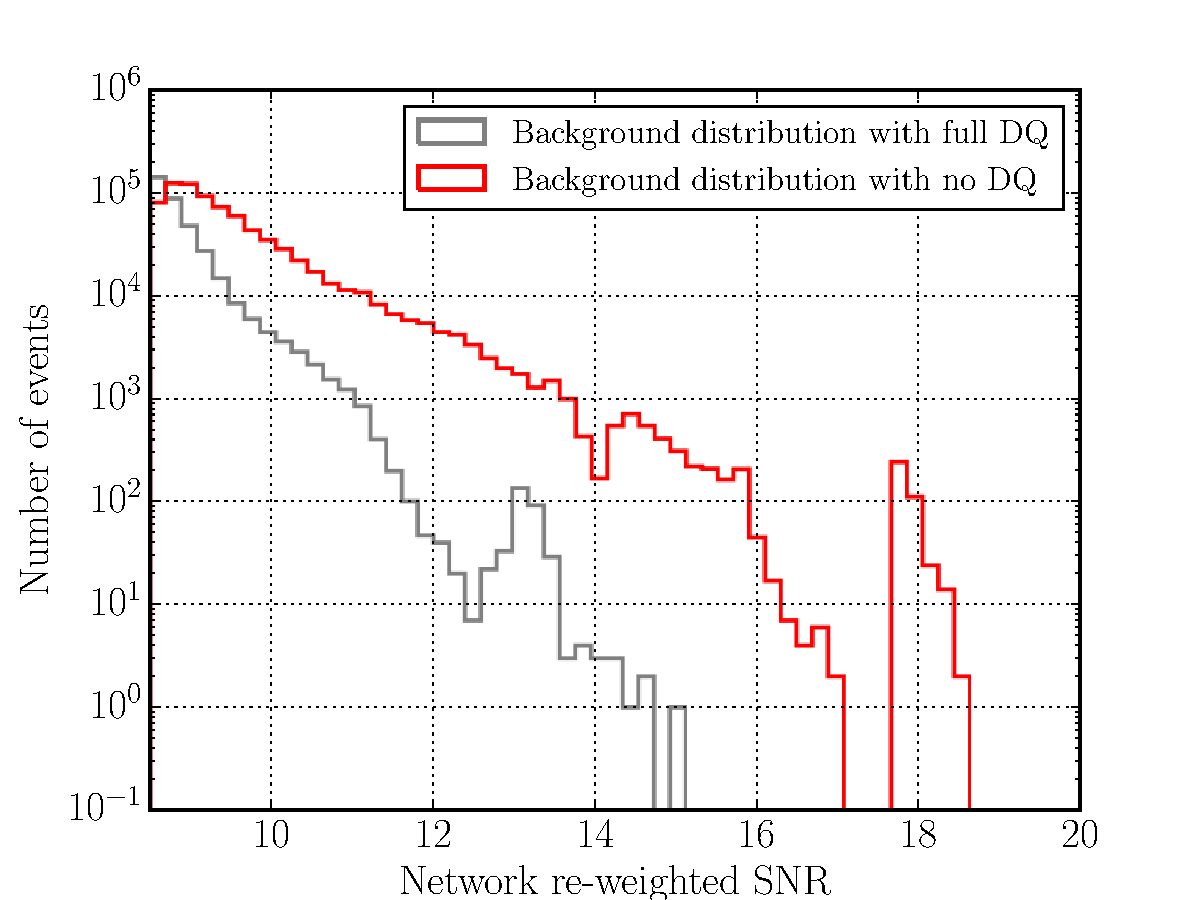
\includegraphics[width=0.495\textwidth]{figures/o1-cbc-dq-paper/edge_bin_GW151226_DQ_raw_hist}
  \label{subfig:edge-bin-gw151226-raw}
  }
  \caption[Edge bin histograms - GW151226 analysis]{The background distribution in the edge bin before and after applying data quality (DQ) vetoes. %
           (\ref{subfig:edge-bin-gw151226-rate}) The cumulative rate of background triggers %
           in the edge bin as a function of re-weighted SNR. %
           (\ref{subfig:edge-bin-gw151226-raw}) A histogram of background triggers %
           in the bulk bin. % 
           The red traces indicate the distribution of background triggers without %
           removing noisy data and the gray traces indicate the distribution %
           of background triggers with all data quality vetoes applied. %
           If noisy data are not removed from the analysis, the tail of loud background  %
           extends to $\hat{\rho}_{c} =$ 18.3.
          }
\label{fig:edge-bin-far-GW151226}
\end{figure}

Further, there is a notable separation between the two background distributions at all
values of $\hat{\rho}_{c}$. This separation can once again be quantified using the
hypothetical detection candidate at $\hat{\rho}_{c} =$ 11.3. Table \ref{table:151226-edge-far}
shows the false alarm rates and probabilities at $\hat{\rho}_{c} =$ 11.3 for various
analysis configurations. When data with excess noise is removed from the analysis, the false
alarm rate at $\hat{\rho}_{c} =$ 11.3 is reduced by a factor of 64.
The application of CAT2 vetoes has an impact in this bin, providing a factor
of 12 reduction in false alarm rate compared to the analysis with only CAT1 vetoes applied.

\begin{table}[!ht]%
  \begin{center}
    \begin{tabular}{lcc}
      \hline
      Analysis configuration & False alarm rate ($yr^{-1}$) & False alarm probability \\ \hline
      All vetoes applied & $1.70\times10^{-3}$  & $7.08\times10^{-5}$ \\
      No CAT2 applied & $2.16\times10^{-2}$ & $9.16\times10^{-4}$ \\
      No CAT1 or CAT2 applied & $0.108$ & $4.77\times10^{-3}$ \\ \hline
    \end{tabular}
  \end{center}
  \caption[Edge bin FAR - GW151226 analysis]{Table of false alarm rates and probabilities at $\hat{\rho}_{c} =$ 11.3 %
           for several analysis configurations. The application of CAT2 vetoes %
           has an effect in this bin, providing a factor of 12 reduction in false %
           alarm rate. Applying all data quality vetoes provides a factor of 64 %
           reduction in false alarm rate.}
  \label{table:151226-edge-far}
\end{table}




\Chapter{Limiting Noise Sources in the PyCBC Search}
\label{ch:CBCDetCharLimits}
What are the current limiting noise sources?

\section{Loud transients}

\subsection{Do loud instrumental transients contribute to the newSNR tail?}

\section{Blip glitches}

\subsection{Time-frequency morphology}

\subsection{Time-domain picture with CBC waveforms}

\subsection{What areas of the CBC parameter space are impacted by blips?}

\section{60-200 Hz noise}

\subsection{Time-frequency morphology}

\subsection{What areas of the CBC parameter space are impacted?}




\Chapter{Conclusion}
\label{ch:Conclusion}
Advanced LIGO's first observing run was highly successful, resulting in the first direct detection of 
gravitational waves and further tests of Einstein's General Theory of Relativity. Gravitational waves 
from two binary black hole mergers, GW150914 and GW151226, were measured at the LIGO interferometers 
and recovered from the data using matched filter search algorithms. 

Searching for gravitational waves requires an understanding of instrumental
features and artifacts that can adversely affect the output of a gravitational wave
search pipeline. Throughout the observing run, data quality vetoes were produced
to ensure that the analysis pipelines analyzed clean data \cite{GW150914-DETCHAR}.

Data quality vetoes improved the sensitivity of the PyCBC search in Advanced LIGO's first
observing run. Although the BNS bins were not dramatically affected, the distribution
of background events was notably improved in the bulk and edge bins.
In both bins, a significant tail of loud background triggers appeared
if noisy data were not removed from the search.

In all 3 bins, it is evident that CAT1 vetoes had a more significant impact on false alarm rates
than CAT2 vetoes, often providing 2-3 orders of magnitude of improvement in false alarm rate in the bulk
and edge bins. This is expected, given that CAT1 vetoes are used to remove the most egregious
data from the analysis. CAT2 vetoes had the greatest impact in the bulk and edge bins from the
analysis containing GW151226, providing at least one order of magnitude reduction in false alarm
rate compared to analyses using CAT1 vetoes only. This is due to a particularly effective CAT2 flag that
was implemented in the
analysis containing GW151226, but was not relevant during the analysis containing GW150914.

The black hole binary system GW150914 was a strong enough signal that it was louder than all background
events regardless of what data were removed from the search. As such, data quality vetoes did not
improve its significance.
The significance of LVT151012 was improved when data with excess noise were removed. Its
false alarm rate was improved from 3.09 $\mathrm{yr}^{-1}$ to 0.44 $\mathrm{yr}^{-1}$ when data quality vetoes were applied
to the PyCBC search.

The significance of the second binary black hole system discovered in O1, GW151226, was significantly
increased by the application of data quality vetoes. The false alarm rate of GW151226 decreases by a
factor of 567 when data quality vetoes are applied, which results in a clear detection ($>$5$~\sigma$) from a
marginal detection candidate (3.9$~\sigma$).


\appendix
\Chapter{Data Quality Vetoes in O1}
\label{ap:o1vetoes}
This document describes all the data quality (DQ) vetoes which were applied to
the analysis of GW150914. For each DQ flag the definition of the veto is given,
the interferometer this veto is applicable to, the category the veto was
applied to the Burst and Compact Binary Coalescence (CBC) searches and the
total amount of deadtime associated to each DQ veto. This document has been
created as a supplement to LIGO-P1500238.

\section{Data Quality Vetoes}

\textbf{Missing Data Veto} \\
\textbf{Purpose}: This veto captures any data dropouts at either interferometer.\\
\textbf{Definition}: Customized software indicate when the recalibrated data
frames were unable to be produced either due to missing raw interferometer data
or data in the raw data frames that are marked as invalid.\\
\textbf{Veto Category}: Burst - 1, CBC - 1\\
\textbf{Deadtime:} LIGO-Hanford - 0\%, LIGO-Livingston - 0\%
\\

\textbf{Burst Hardware Injection Veto} \\
\textbf{Purpose}: This veto indicates whenever a burst hardware injection has
been performed.\\
\textbf{Defintion}: The times of transient hardware injections labelled as
burst type are recorded by the online detector characterization (ODC) system by
monitoring the state of the calibration injection model. Deadtime quoted
includes the padding used in the analyses ($\pm$4 seconds).\\
\textbf{Veto Category}: Burst - 4\footnote{Burst veto category 4 is reserved
for transient hardware injections only.}, CBC - 2\\
\textbf{Deadtime:} LIGO-Hanford - 0.003\%, LIGO-Livingston - 0\%
\\

\textbf{CBC Hardware Injection Veto} \\
\textbf{Purpose}: This veto indicates whenever a CBC hardware injection has
been performed.\\
\textbf{Defintion}: The times of transient hardware injections labelled as CBC
type are recorded by the ODC system by monitoring the state of the
calibration injection model. Deadtime quoted includes the padding used in the
analyses ($\pm$8 seconds).\\
\textbf{Veto Category}: Burst - 4, CBC - 3\footnote{CBC veto category 3 is
reserved for CBC hardware injections only.}\\
\textbf{Deadtime:} LIGO-Hanford - 0.052\%, LIGO-Livingston - 0.072\%
\\

\textbf{DetChar Hardware Injection Veto} \\
\textbf{Purpose}: This veto indicates whenever a DetChar hardware injection has
been performed.\\
\textbf{Defintion}: The times of transient hardware injections labelled as
DetChar type are recorded by the ODC system by monitoring the state of the
calibration injection model. Deadtime quoted includes the padding used in the
analyses ($\pm$16 seconds).\\
\textbf{Veto Category}: Burst - 4, CBC - 2\\
\textbf{Deadtime:} LIGO-Hanford - 0\%, LIGO-Livingston - 0\%
\\

\textbf{Stochastic Hardware Injection Veto} \\
\textbf{Purpose}: This veto indicates whenever a stochastic hardware injection
has been performed.\\
\textbf{Defintion}: The times of hardware injections labelled as
stochastic type are recorded by the ODC system by monitoring the state of the
calibration injection model.\\
\textbf{Veto Category}: Burst - 1, CBC - 1\\
\textbf{Deadtime:} LIGO-Hanford - 0\%, LIGO-Livingston - 0\%
\\

\textbf{Beckhoff Hardware Problems} \\
\textbf{Purpose}: To capture times when the Beckhoff system (a slow control
system which is used to control a subset of hardware in the interferometer)
suffered a hardware failure at the LIGO-Hanford Y-end. \\
\textbf{Defintion}: The veto was created by hand, where the start time was
recorded as 4 seconds before excess non-stationary data started due to the
hardware failure and finished 3 seconds after the interferometer dropped out of
observing mode.\\
\textbf{Veto Category}: Burst - 1, CBC - 1\\
\textbf{Deadtime:} LIGO-Hanford - 1.50\%
\\

\textbf{45 MHz Sideband Fluctuations} \\
\textbf{Purpose}: This veto identifies times when the amplitude of the 45 MHz
optical sideband, which is used to generate error signals for optical cavities,
has excess noise. If the amplitude of the 45 MHz optical sideband fluctuates,
excess noise will be injected in to the associated optical cavities which has
been seen to couple to the gravitational wave channel.\\
\textbf{Defintion}: An auxiliary channel which monitors amplitude fluctuations
in the signal used to generate the 45 MHz optical sideband was found to be the
optimum witness of non-stationary behaviour seen in the gravitational wave
channel data. This veto was designed to capture long duration (on the order of
one minute) non-stationary behaviour. Various thresholds on the band limited
root-mean-square of this
witness channel were investigated to see which threshold proved most effective
(in terms of efficiency and deadtime) at removing non-stationary data.
Custom software was implemented to automatically capture this behaviour over
the analysis period (and throughout the first observing run).\\
\textbf{Veto Category}: Burst - 1, CBC - 1\\
\textbf{Deadtime:} LIGO-Hanford - 2.95\%
\\

\textbf{Less severe 45 MHz Sideband Fluctuations} \\
\textbf{Purpose}: See above veto, 45 MHz sideband fluctuations, for
description.\\
\textbf{Defintion}: This veto was designed to capture less severe, short time
scale (on the order of 1 second), non-stationary data. This veto was created
in a similar manner as the previous veto - a study of different thresholds
on the band limited root-mean-square of the witness channel were investigated
to give the optimal efficiency and deadtime. Custom software was implemented to
automatically capture this behaviour over the analysis period (and throughout
the first observing run).\\
\textbf{Veto Category}: Burst - not applied, CBC - 2\\
\textbf{Deadtime:} LIGO-Hanford - 0.014\%
\\

\textbf{Saturations in the SUSETMY model channels} \\
\textbf{Purpose}: This veto captures time when the Y-end test mass actuator
saturates. This is due to a relatively fast transient that is on the main
carrier beam, and therefore directly on/at the readout, which gets amplified
by the differential-arm digital filters sufficiently to cross the
digital-to-analog converter limits.\\
\textbf{Defintion}: This veto was created automatically by monitoring the
interface between the computers and the analog electronics that they control on
the Y-end test mass.\\
\textbf{Veto Category}: Burst - 2, CBC - 2\\
\textbf{Deadtime:} LIGO-Hanford - 0.067\%, LIGO-Livingston - 0.021\%
\\

\textbf{Saturations in the SUSETMY model channels with an SNR $>$ 200} \\
\textbf{Purpose}: See veto above - saturations in the SUSETMY model channels.
This veto however is aimed specifically to identify very loud saturations.\\
\textbf{Defintion}: This veto was created automatically by monitoring the
interface between the computers and the analog electronics that they control on
the Y-end test mass. A subset of these saturations is kept based on their
severity as determined by an algorithm that is designed to witness transient
power in a given signal. This veto is specific to the Burst search where
$\pm$3 seconds of padding is applied.\\
\textbf{Veto Category}: Burst - 2, CBC - not applied\\
\textbf{Deadtime:} LIGO-Hanford - 0.146\%, LIGO-Livingston - 0.047\%
\\

\textbf{Output Mode Cleaner (OMC) Photodiodes Analog to Digital Overflows} \\
\textbf{Purpose}: This veto captures times when the signal on the OMC
photodiodes exceeds the limit of the analog-to-digital converter at the
interface to the computers that control the instrument.\\
\textbf{Defintion}: This veto was created automatically by monitoring the
interface between the OMC photodiodes analog signal and the computers.\\
\textbf{Veto Category}: Burst - 2, CBC - 2\\
\textbf{Deadtime:} LIGO-Hanford - 0.002\%, LIGO-Livingston - 0.003\%
\\

\textbf{Non-Stationary Data prior to Loss of Resonant Power in the Optical Cavities} \\
\textbf{Purpose}: To veto times when the data became non-stationary before the
state of the interferometer reported the end of an observation segment.\\
\textbf{Defintion}: These times were found by hand by monitoring an algorithm,
run over the gravitational wave channel, that is designed to witness transient
power. \\
\textbf{Veto Category}: Burst - 1, CBC - 1\\
\textbf{Deadtime:} LIGO-Hanford - 0.0004\%, LIGO-Livingston 0.001\%
\\

\textbf{Glitches due to DC Power Fluctuations of the Photon Calibrator Laser} \\
\textbf{Purpose}: This veto captures times when the photon calibrator has
power fluctuations which exceed 20\% of the nominal level.\\
\textbf{Defintion}: A threshold placed on a witness channel which monitors the
power levels of the photon calibrator laser was used to flag
times when the power fluctuated beyond the 20\% level. These times were then
padded by -10 and +20 seconds to capture the full behaviour.\\
\textbf{Veto Category}: Burst - 1, CBC -1\\
\textbf{Deadtime:} LIGO-Livingston - 0.058\%
\\

\textbf{Seismic Glitches} \\
\textbf{Purpose}: This veto was created to identify times of strong excess
seismic noise that coupled in to the output of the interferometer.\\
\textbf{Defintion}: The 10-30 Hz band limited root-mean-
square of the ground seismometer, located at the input test mass on the Y-arm, in the vertical degree of freedom was found to correlate with excess noise in
the output of the interferometer. Different thresholds on this witness channel
were tested to find the optimal efficiency and deadtime that captured these
effects.\\
\textbf{Veto Category}: Burst - not applied, CBC - 2\\
\textbf{Deadtime:} LIGO-Hanford - 0.431\%




\clearpage
\bibliographystyle{unsrt}
\bibliography{references,cbc-group,updated_refs,GW150914_refs}

\addcontentsline{toc}{chapter}{\numberline {Bibliography}}

\clearpage
\birthplacedate{Rochester, NY \>\>July 22, 1989}
\collegewherewhen{%
\>Utica College \>\>2007--2011, \>B.S.\\
\>\su	\>\>2011--2016, \>Ph.D.}

\newpage
\null\vskip1in%
\begin{center}
{\Large\bf Curriculum Vitae}
\end{center}
\vskip 2em
\begin{tabbing}
\tabset
Title of Dissertation\\
\>Detector Characterization of Advanced LIGO
\end{tabbing}
\vskip 1em

\begin{startvita}
\end{startvita}

\renewenvironment{thebibliography}[1]%
  {\begin{list}{\labelenumi\hss}%
     {\usecounter{enumi}\setlength{\labelwidth}{3em}%
      \setlength{\leftmargin}{5em}}}%
  {\end{list}}
\renewcommand{\bibitem}[1]{\item\label{#1}\relax}%
\renewcommand{\theenumi}{\arabic{enumi}}%
%\begin{publications}
%\putbib[papers]
%\end{publications}


\finishvita
\end{document}
